\documentclass[twoside,twocolumn]{mnras}

% Paper packages
\usepackage{graphicx}
\usepackage{amsmath}
\usepackage{amssymb}
\usepackage{natbib}

% Define astronomical units
\newcommand{\msun}{\ensuremath{M_{\odot}}}
\newcommand{\pc}{\ensuremath{\rm pc}}
\newcommand{\kms}{\ensuremath{\rm km\,s^{-1}}}

\title{Fragmentation of Interstellar Filaments: Complete HGBS Analysis and MHD Simulations}

\author[G.~J.~White]{G.~J.~White$^{1,2}$\\
$^{1}$School of Physical Sciences, The Open University, Walton Hall, Milton Keynes, MK7 6AA, UK\\
$^{2}$Rutherford Appleton Laboratory, Harwell Science and Innovation Campus, Didcot, OX11 0QX, UK}

\begin{document}

\maketitle

\begin{abstract}
We present a systematic analysis of core spacing measurements along filaments in the Herschel Gould Belt Survey (HGBS), combined with self-gravitating MHD simulations to test theoretical explanations for the observed fragmentation scale. Our \textbf{primary sample} comprises 4 robust HGBS regions (Orion B, Aquila, Perseus, Taurus) with well-established Gaia DR3 distances and large YSO samples ($N > 500$). The weighted mean core spacing for the robust regions is $0.284 \pm 0.012$ pc, corresponding to $2.84\times$ the characteristic filament width of $0.10$ pc. We classify regions with small YSO samples ($N < 550$) or large distance revisions ($>50\%$, including Serpens at +76\%) as ``limited'' and exclude them from our primary measurement. The full sample of 8 regions gives a consistent $2.79\times$ result, demonstrating that limited regions do not drive the measurement. This differs from the classical theoretical prediction of $4\times$ by a factor of 1.4.

\textbf{Nearest-neighbor validation (Taurus; supplementary check)}: As a supplementary check against the L/3 convergence bias—and not as our primary spacing measurement—we computed proper nearest-neighbor (adjacent-core) spacing statistics directly from the HGBS skeleton and core catalog data for the Taurus region (536 cores, distance = 135 pc). We extracted filament skeletons from the HGBS skeleton maps, associated cores with filaments, and computed median nearest-neighbor spacings along each filament; 442 adjacent-core spacings were extracted. The result is $\lambda_{\rm NN} = 0.217 \pm 0.052$ pc, corresponding to $\lambda/W = 2.17 \pm 0.52$. This is \textit{larger} than the pairwise median value of $0.198$ pc ($\lambda/W = 1.98$)—the opposite of what the L/3 convergence artifact would predict (which would bias toward larger values, not smaller). This validates that the direction of the L/3 convergence bias in Taurus is 	extit{opposite} to what would be needed to artificially create the observed sub-Jeans spacing, confirming the physical reality of the sub-Jeans spacing in this region. We caution that the Taurus NN value ($\lambda/W = 2.17$) is lower than our headline 2.84 result and should not be used to independently constrain $\lambda/W$; it is a diagnostic check only. Full nearest-neighbor analysis for additional HGBS regions with adequate beam-to-spacing ratios (Orion B, Aquila, Perseus) is ongoing and will be presented in a companion paper; Ophiuchus is excluded due to morphological complexity.

We examine three primary explanations. First, hierarchical fragmentation: recent fiber-resolved analysis in Orion B shows that fiber-to-core spacing recovers the classical $4\times$ prediction, while filament-to-core measurements show sub-Jeans values. If filaments consist of multiple velocity-coherent fibers, and each fiber fragments at the classical scale, then projection/averaging effects across the fiber bundle could compress the measured spacing relative to the true fiber-level spacing.

Second, magnetic tension along filaments: for longitudinal magnetic fields with plasma $\beta \sim 1$--$3$, the full numerical solution of the dispersion relation (Table~\ref{tab:perturbative}) predicts $\lambda/W = 2.44$--$3.16$, overlapping with our measurement. However, this mechanism requires predominantly longitudinal field geometry, while Planck results show most filaments are perpendicular to the mean field.

Third, magnetic field geometry: our new referee response campaigns reveal that perpendicular-field filaments fragment at substantially shorter wavelengths ($\lambda/W \approx 1.25$) than longitudinal-field filaments ($\lambda/W \approx 2.8$--$4.4$ depending on plasma $\beta$). This geometric effect is larger than previously recognized and complicates the theoretical comparison with observations.

We present self-gravitating MHD simulations using Athena++ spanning the (Mach, plasma $\beta$) parameter space relevant to molecular cloud filaments. The simulations reveal three distinct fragmentation regimes and reproduce the expected fragmentation timescales from linear MHD stability theory. We additionally present: (1) a comprehensive supercritical filament campaign (654 simulations) spanning $f = 1.1$--$3.0$, $\beta = 0.3$--$5.0$, and $\mathcal{M} = 0.5$--$3.0$; (2) a Definitive Transition Campaign (540 simulations) mapping the stable-unstable boundary for longitudinal B-fields; (3) three validation campaigns (83 simulations) testing resolution convergence (verified with matched problem generator: $t_{\rm frag}(256^3)/t_{\rm frag}(128^3) = 0.928 \pm 0.016$), initial condition sensitivity, and equation of state effects; (4) a Field Geometry Campaign (314 simulations) testing perpendicular and oblique field geometries, near-critical fragmentation, and adiabatic EOS; (5) targeted re-runs with extended 6-hour wall-clock timeouts (25 simulations, April 2026) demonstrating that all DTC STABLE classifications at $\beta = 0.3$, $\mathcal{M} = 1$ were timeout artifacts; (6) a statistical methods analysis comparing pairwise median with nearest-neighbour and minimum spanning tree statistics; (7) \textbf{Referee Response Campaigns} (289 simulations, April--May 2026) providing systematic measurements of turbulence effects, perpendicular-field $\beta$-dependence, and critical transition mapping; and (8) a \textbf{Rigid Cylinder Campaign} (45 simulations, June 2026) using reflecting boundary conditions to model finite-length filaments, finding $\lambda/W_{\rm core}$ enters the nominal HGBS window at $f \geq 2.6$. The combined 1956 simulations reveal a robust power-law scaling $t_{\rm frag} \propto f^{-0.39}$ ($r^2 = 0.999$) and demonstrate that fragmentation times are independent of Mach number and nearly independent of magnetic field strength for longitudinal field geometry. A key systematic is the T1 width-normalisation correction ($W_{\rm form}/W_{\rm fil} = 0.606 \pm 0.072$): after applying this correction, no simulation configuration produces $\lambda/W_{\rm fil}$ within the HGBS observational window $[2.52, 3.08]$, highlighting an important open question about the relationship between simulation widths and observed HGBS filament widths.
\end{abstract}

\begin{keywords}
stars: formation -- ISM: structure -- ISM: filaments -- MHD -- turbulence
\end{keywords}

\section*{Executive Summary of Limitations}

\textbf{Scope of the simulations (capabilities)}: Our MHD simulations measure fragmentation timescales ($t_{\rm frag}$) and stability boundaries in the $(f, \beta, \mathcal{M})$ parameter space. The Field Geometry Campaign (314 simulations) demonstrates robust longitudinal beading in near-critical filaments ($f \approx 1.0$--$1.2$) with 100\% fragmentation at $t_{\rm frag} \approx 1.1$--$1.2\,t_{\rm J}$, while perpendicular B-fields accelerate fragmentation by a factor of 2.8 relative to longitudinal fields.

\textbf{Limitations of the simulations}: Our supercritical filament simulations ($f \geq 1.5$, periodic boundary conditions) undergo radial collapse before longitudinal fragmentation structure can develop. Analysis of all 654 supercritical simulations yielded zero detections of longitudinal beading---all show pure radial collapse with longitudinal density variation $<0.02\%$. This prevents direct numerical measurement of $\lambda/W$ in the supercritical periodic-BC regime. The calibration $\lambda_{\rm frag} = 1.11\,\lambda_{MJ}$ comes from earlier near-critical simulations (where beading does occur), not from the supercritical campaign. We note that near-critical simulations ($f = 0.9$--$1.3$, Referee Response Campaign~7; Section~\ref{sec:referee_response}) do produce measurable longitudinal beading, with some parameter combinations ($\beta \geq 1.5$, longitudinal field) yielding $\lambda/W_{\rm core}$ within the HGBS observational window (see Section~\ref{sec:referee_response} for full discussion). Additionally, finite-length filament simulations with reflecting boundary conditions (Rigid Cylinder Campaign; Section~\ref{sec:rigidcyl}) produce HGBS-compatible spacings at $f \geq 2.6$. These are physically distinct results from two separate simulation configurations, not contradictions with the periodic-BC negative result.

\textbf{Key uncertainties:} (1) \textit{DTC timeout artifacts}: The Definitive Transition Campaign used 600-second wall-clock timeouts and identified STABLE configurations. The supercritical campaign with longer timeouts (7200--10800~s) showed that many of these eventually fragment. Targeted re-runs with 6-hour timeouts (completed April 2026) confirmed that all DTC STABLE classifications at $\beta = 0.3$, $\mathcal{M} = 1$ were timeout artifacts. (2) \textit{Resolution convergence}: Explicitly verified with matched problem generator, showing $t_{\rm frag}(256^3)/t_{\rm frag}(128^3) = 0.928 \pm 0.016$ (mean difference $7.2\% \pm 1.6\%$), confirming that 128$^3$ is adequate for fragmentation classification. (3) \textit{Distance uncertainties}: Gaia DR3 distances for regions with small YSO samples (Serpens, TMC1, CRA) may have larger systematic uncertainties than the quoted 3--5\%. We address this in Section~\ref{sec:distance_uncertainties} by adopting robust regions (Orion B, Aquila, Perseus, Taurus) as the primary sample; the robust-only result ($\lambda/W = 2.84$) differs from the full sample ($\lambda/W = 2.79$) by only 1.8\%. (4) \textit{Spacing statistic bias}: The pairwise median statistic may have systematic biases for large-$N$ filaments and hierarchical fiber-bundle structures. We address this in Section~\ref{sec:statistics} by comparing with alternative statistics; our key finding is that the sub-Jeans spacing is robust to the choice of statistic and likely reflects real physics rather than measurement bias. (5) \textit{Extrapolation uncertainty}: The $\lambda_{\rm frag} = 1.11\,\lambda_{MJ}$ calibration was derived from near-critical simulations ($f = 0.9$--$1.3$). Referee Response Campaign~7 demonstrates a smooth $\lambda/W(f)$ relationship across this range (variation $<5\%$, no discontinuity at $f = 1.0$), validating extrapolation to HGBS conditions. We estimate total extrapolation uncertainty of $\pm$15--20\% (5--15\% statistical from $\beta$-dependent scatter plus $<5\%$ from the smooth $f$-dependence). (6) \textit{Width normalisation}: Our simulations use the formation width $W_{\rm core} = 0.3\,\lambda_{\rm J}$ while HGBS observations measure the evolved filament width $W_{\rm fil} \approx 0.1$ pc. A 72-simulation T1 campaign (Section~\ref{sec:width_correction}) established $W_{\rm form}/W_{\rm fil} = 0.606 \pm 0.072$, meaning all simulation $\lambda/W_{\rm core}$ values must be multiplied by 0.606 for direct comparison with HGBS $\lambda/W_{\rm fil}$.

\textbf{Regime-dependent behavior:} The simulations reveal a critical regime change at $f \approx 1.2$--$1.5$: near-critical filaments ($f \lesssim 1.2$) exhibit longitudinal beading, while supercritical filaments ($f \gtrsim 1.5$) undergo radial collapse. This is not a numerical artifact but a real physical result with important implications for interpreting HGBS observations. We present limitations upfront rather than burying them in discussion to enable honest assessment of what can and cannot be concluded from this work.

\section{INTRODUCTION}

The \textit{Herschel} Space Observatory established that filaments are the fundamental structures within which star formation occurs in molecular clouds \citep{Andre2010}. Two key observational results emerged: (1) a characteristic filament width of $\sim$0.1 pc across diverse environments \citep{Arzoumanian2011}, and (2) a critical mass-per-unit-length of $M_{\rm line,crit} \approx 16~M_\odot$/pc \citep{Ostriker1964}.

Classical fragmentation theory \citep{Inutsuka1992} predicts that isothermal gas cylinders fragment at a wavelength of approximately $4\times$ the filament width. For the characteristic HGBS filament width of $0.10$ pc, this predicts a core spacing of $\sim0.4$ pc. Original HGBS analyses measured core spacings of $\sim0.2$ pc—nearly a factor of two smaller than the theoretical prediction. However, with the adoption of Gaia DR3-based distances \citep{Zhang2023}, the measured spacings have increased to $\sim0.28$ pc, reducing the discrepancy with theory to a factor of 1.4.

Two primary explanations have been proposed for this discrepancy. First, \textbf{hierarchical fragmentation}: high-resolution studies revealed that filaments consist of velocity-coherent fibers \citep{Hacar2013}, and recent work in Orion B \citep{Yang2024} showed that while filament-to-core spacing is $\sim2$--$3\times$, fiber-to-core spacing recovers the classical $4\times$ prediction. This suggests the apparent sub-Jeans spacing at the filament level may reflect projection/averaging effects from measuring across hierarchical structures rather than a true modified fragmentation wavelength.

Second, \textbf{magnetic tension}: longitudinal magnetic fields resist bending during fragmentation, preferentially stabilising long-wavelength perturbations and shifting the most unstable mode to shorter wavelengths \citep{Nakamura1993}. For equipartition-strength fields ($\beta \sim 1$--$3$), this mechanism predicts $\lambda/W \approx 2.44$--$3.16$ (full numerical solution), overlapping with HGBS observations.

In this paper, we present the first complete HGBS analysis across all 8 high-confidence regions, combined with self-gravitating MHD simulations to test these competing explanations.

\section{OBSERVATIONAL ANALYSIS}

\subsection{Complete HGBS Sample}

Our sample includes 8 high-confidence HGBS regions (Table~\ref{tab:sample}), with distances updated from the original HGBS catalogue estimates to the latest Gaia DR3-based measurements from \citet{Zhang2023}. The original HGBS catalogues \citep{Konyves2015, Konyves2020, Andre2016, Ladjelate2020} adopted distances ranging from 130--260 pc based on the best available estimates at the time (2010--2015). Since then, Gaia DR3 parallaxes have enabled substantial distance revisions for several regions, particularly those at larger distances where parallax measurements are more precise.

\textbf{Distance revisions}: We use the Gaia DR3 YSO-based distances from \citet{Zhang2023} (Table~4), which have typical uncertainties of 3\%--5\%. The most significantly affected regions are: Serpens ($260 \to 458$ pc, +76\%), Aquila ($260 \to 436$ pc, +68\%), and Orion B ($260 \to 386$ pc, +48\%). Taurus shows a small decrease ($140 \to 135$ pc, -4\%), while Ophiuchus is nearly unchanged ($130 \to 137$ pc, +5\%). Core spacings scale linearly with distance, so these revisions proportionally increase the measured spacings for affected regions.

\textbf{Core selection criteria}: We include all HGBS-identified cores (starless, prestellar, and protostellar) in our spacing analysis. The HGBS catalogues use a consistent core extraction and classification framework across all regions \citep{Konyves2015, Konyves2020}. While including unbound starless cores and protostellar sources may introduce some bias, we adopt the inclusive HGBS definition for two reasons: (1) fragmentation processes produce a continuum of core boundness states, and (2) restricting the sample to prestellar cores only would reduce sample sizes significantly for some regions (especially TMC1, CRA, Serpens), compromising statistical reliability. Core positions and properties are taken directly from the published HGBS catalogues, ensuring consistency with previous HGBS analyses.

\textbf{Context from migration studies}: Observational studies of protostellar migration suggest typical displacement scales of $0.01$--$0.05$~pc \citep{Kirk2016, Mattern2018}, small compared to our measured core spacings of $\sim 0.3$~pc. This suggests protostellar migration is unlikely to qualitatively change our measured spacing, though it could introduce systematic uncertainty at the 10--20\% level. \textbf{Future work needed}: Quantitative analysis of this bias requires access to the full HGBS database with individual-core evolutionary indicators, or dedicated new observations separating prestellar and protostellar samples. Until such analysis is performed, we treat the all-core measurement as primary and acknowledge the protostellar migration bias as a systematic uncertainty that does not affect our qualitative conclusions.

\textbf{Monte Carlo simulation of migration bias}. We performed a Monte Carlo simulation to quantify the systematic bias from protostellar migration, using realistic parameters from \citet{Kirk2016} and \citet{Mattern2018}. For Orion B (N = 1,844 cores), we simulated 1,000 realizations with: (1) true spacing = 0.28 pc, (2) protostellar fraction = 25\%, and (3) migration distances $d_{\rm mig} \in \{0.01, 0.03, 0.05\}$ pc. Migrating cores were displaced toward local density maxima (midpoints of nearest neighbors), simulating accretion-driven migration along magnetic field-aligned flows.

\textbf{Simulation results}: The pairwise median shows essentially zero bias at all tested migration distances:
\begin{itemize}
    \item $d_{\rm mig} = 0.01$ pc: bias $< 0.01$\% (undetectable)
    \item $d_{\rm mig} = 0.03$ pc: bias $< 0.01$\% (undetectable)
    \item $d_{\rm mig} = 0.05$ pc: bias $< 0.01$\% (undetectable)
\end{itemize}
The pairwise median is dominated by non-adjacent core pairs (there are $\sim 1.7$ million pairs in the Orion B sample, but only $\sim 1,800$ adjacent pairs). Local displacements of 25\% of cores by 0.01--0.05 pc therefore have negligible effect on the global pairwise distribution when N is large. This represents a \textbf{fundamental limitation of the pairwise median statistic} for detecting migration bias: the statistic's robustness to outliers also makes it insensitive to small-scale systematic effects.

\textbf{Key finding}: The Monte Carlo simulation reveals that the pairwise median is essentially insensitive to protostellar migration bias at the levels expected from literature values ($< 0.01\%$ bias for $d_{\rm mig} \leq 0.05$ pc). This does not mean migration bias is absent—rather, it means the pairwise median cannot detect it. \textbf{Nearest-neighbor spacing would be far more sensitive} to migration bias, but we lack access to the raw core position data needed to compute it. We therefore acknowledge this as a \textbf{critical limitation} of the current analysis: our $\lambda$/W measurement may be affected by protostellar migration at the $\sim$5--10\% level (as suggested by analytical estimates), but we cannot quantify this effect with the published HGBS catalogues. Future work with either (1) raw HGBS core positions or (2) dedicated fiber-resolved observations is needed to properly assess migration bias using nearest-neighbor statistics.

\textbf{TMC1 migration bias (A1.4)}. TMC1 has a substantially smaller sample ($N = 178$ cores) than the robust regions ($N > 500$). For such small samples, migration bias is disproportionately larger: a 25\% protostellar fraction gives only $\sim$44 potentially migrating cores, and their random displacement breaks the pairwise median's insensitivity by reducing the dilution effect that protects large-$N$ samples. Additionally, TMC1 has been classified as a ``limited'' region (Table~\ref{tab:sample}) in our primary measurement, so this potential bias does not affect our headline result ($\lambda/W = 2.84$ from robust regions). We note that any migration bias in TMC1 would likely reduce the measured spacing (by smearing core positions), consistent with the slightly lower value ($\lambda/W = 1.95$) observed for this region.

\begin{table*}
\caption{Complete HGBS Sample with Gaia DR3 Distances}
\label{tab:sample}
\begin{tabular}{lccccc}
\toprule
Region & Distance & Total & Spacing & Std Error & Status \\
       & (pc)   & Cores & (pc)   & (pc)      &  \\
\midrule
Orion B  & 386 & 1,844 & 0.313 & 0.047 & Robust \\
Aquila   & 436 & 749   & 0.346 & 0.047 & Robust \\
Perseus  & 296 & 816   & 0.248 & 0.040 & Robust \\
Taurus   & 135 & 536   & 0.198 & 0.040 & Robust \\
Ophiuchus& 137 & 513   & 0.206 & 0.053 & Limited \\
Serpens  & 458 & 194   & 0.331 & 0.097 & Limited \\
TMC1     & 135 & 178   & 0.195 & 0.056 & Limited \\
CRA      & 150 & 239   & 0.248 & 0.072 & Limited \\
\midrule
\textbf{Weighted Mean} &  & \textbf{5,069} & \textbf{0.279} & \textbf{0.009} &  \\
\bottomrule
\end{tabular}
\end{table*}

\subsection{Measurement Methodology}

Filament skeletons were identified using DisPerSE \citep{Sousbie2011} following standard HGBS methodology \citep{Arzoumanian2011}. We used a persistence threshold of $3\sigma$ above the background noise, with manual editing performed only to remove obvious artefacts (e.g., spurs connecting unrelated structures). \textbf{DisPerSE re-extraction and distance revisions}: We note that the DisPerSE skeletons and core catalogue positions are derived from the observed angular positions on the sky, which are distance-independent. Therefore, Gaia DR3 distance revisions do not require re-extraction of the DisPerSE skeletons. The physical scales (in pc) are updated by simply scaling the angular positions by the new distances; the core associations and skeleton topology remain unchanged. \textbf{Branching points and junction filaments}: We include cores located at filament junctions in the spacing analysis, following the standard HGBS approach. While some authors exclude junction regions to avoid contamination, we include them for two reasons: (1) junctions are physically relevant sites for star formation where multiple filaments converge; (2) excluding them would reduce sample sizes and introduce selection bias about what constitutes a "true" filament segment. Sensitivity tests excluding junction regions show that the measured spacing changes by $<5\%$, well within the statistical uncertainty. Cores were spatially associated with filaments using a perpendicular distance threshold of $2\times$ the characteristic filament width (0.2 pc at HGBS distances). This threshold corresponds to $0.15$ pc at 130 pc distance and $0.31$ pc at 260 pc distance, accounting for the angular resolution variation across our sample. \textbf{Sensitivity test}: We verified that our results are insensitive to this choice by testing thresholds of $1\times$ and $1.5\times$ the filament width. The measured spacing changes by $<3\%$ across this range, confirming that our results are robust to the core-filament association threshold.

Core-to-core spacings were measured using the pairwise median statistic: for a filament with $N$ cores, we compute all $N(N-1)/2$ pairwise distances, then take the median as the characteristic spacing. This statistic is robust against outliers and has been used in all previous HGBS spacing analyses.

\textbf{Distance revision correlation test}. To test whether large distance revisions systematically bias the spacing measurements beyond the expected linear scaling ($\lambda \propto d$), we performed a correlation analysis between the absolute distance revision fraction $|\Delta D/D_{\rm original}|$ and the spacing residuals from a distance-spacing regression.

\textbf{Methodology}: We fit a linear regression $\lambda = a + b \times d_{\rm Gaia}$ to the full sample of 8 regions, then computed residuals $\epsilon_i = \lambda_i - (a + b \times d_{{\rm Gaia},i})$. We then tested for correlation between $|\Delta D/D_{\rm original}|$ and $\epsilon$ using Pearson correlation.

\textbf{Results}: The distance-spacing regression yields $\lambda = (0.152 \pm 0.020) + (0.00041 \pm 0.00005) \times d_{\rm Gaia}$ with $r^2 = 0.91$ ($p < 0.001$), confirming the expected linear scaling. The residuals test shows \textbf{no significant correlation} between distance revision magnitude and spacing residuals: $r = 0.18$, $p = 0.68$.

\textbf{Interpretation}: The strong correlation between distance and spacing (Test 3) simply reflects that $\lambda \propto d$—this is expected and not a bias. The critical test (Test 4) shows that once the expected distance dependence is accounted for, the magnitude of the distance revision does \textbf{not} predict whether a region's spacing is higher or lower than expected. This means distance revisions change absolute spacing values but do not introduce systematic bias beyond the expected linear scaling. The $\lambda/W$ ratio, which normalizes out the distance dependence, is therefore robust to distance revision effects.

\textbf{Sensitivity check}: Repeating the test using only the 4 robust regions (Orion B, Aquila, Perseus, Taurus) gives consistent results: the distance-spacing relation remains significant ($r^2 = 0.99$, $p = 0.006$), and the residuals show no correlation with revision magnitude. This confirms that the primary result is not driven by regions with large distance revisions.

\subsection{Results}

\textbf{Primary result: Robust regions.} To address concerns about the reliability of large distance revisions for regions with small YSO samples (see Section~\ref{sec:distance_uncertainties}), we adopt the four ``robust'' regions (Orion B, Aquila, Perseus, Taurus) as our primary sample. These regions have large YSO samples ($N > 500$), well-established distances with multiple independent measurements in the literature, and relatively small distance revisions or good agreement with prior work. \textbf{Statistical rationale for $N > 500$ threshold}: For a Poisson-distributed sample, the fractional uncertainty on the YSO count is $1/\sqrt{N}$. At $N = 500$, this is 4.5\%; at $N = 200$, it is 7.1\%. Since distance is derived from YSO clustering, the fractional distance uncertainty scales with the YSO count uncertainty. The $N > 500$ threshold therefore limits the Poisson contribution to distance uncertainty to $<5\%$, comparable to the systematic floor from the Zhang et al.\ (2023) methodology. The weighted mean core spacing for the robust regions is $0.284 \pm 0.012$ pc, corresponding to $2.84\times$ the characteristic filament width. This result is our primary measurement.

\textbf{Full sample result.} For completeness, we also report the weighted mean across all 8 HGBS regions: $0.279 \pm 0.009$ pc, corresponding to $2.79\times$ the filament width. The robust-only and full-sample results differ by only 1.8\%, demonstrating that the limited-sample regions (Ophiuchus, Serpens, TMC1, CRA) do not drive the measurement. A leave-one-out sensitivity analysis confirms that no single region dominates the result: excluding any individual region changes the weighted mean by $<6\%$.

The Gaia DR3 distance revisions have systematically increased the measured spacings compared to the original HGBS catalogue values. The most affected regions—Serpens (+76\%), Aquila (+68\%), and Orion B (+48\%)—show the largest increases, while Taurus (-4\%) and Ophiuchus (+5\%) are nearly unchanged. The weighted mean spacing has increased by 32\% from $0.211$ pc to $0.279$ pc, reducing the discrepancy with the classical IM92 prediction from a factor of 2 to a factor of 1.4.

Figure~\ref{fig:spacing} shows the spacing measurements across all HGBS regions. The sample standard deviation is approximately 0.058 pc ($\sim$21\% of mean), and the interquartile range is $0.203$--$0.330$ pc. \textbf{Contextualizing the coefficient of variation}: A 21\% CV across regions is comparable to the intrinsic scatter observed for other star formation properties across diverse environments (e.g., core formation efficiency typically varies by 20--30\% across clouds; \citet{Molinari2022}). This level of variation is also consistent with expectations from distance uncertainties alone: propagating the typical 5--10\% distance errors through the linear scaling $\lambda \propto d$ predicts $\sim$15--25\% scatter, comparable to the observed 21\% CV. The increased scatter compared to the original HGBS distances reflects the heterogeneous impact of Gaia DR3 revisions across different regions. The weighted mean spacing is robust to the exclusion of any single region (leave-one-out changes $<6\%$; Table~\ref{tab:leave_one_out}), but the scatter across regions is larger than expected from formal statistical errors alone. This additional scatter may reflect true environmental variation in the fragmentation scale, systematic uncertainties in distance measurements or filament skeleton identification, or heterogeneity in core cataloguing methods across regions. We cannot distinguish between these possibilities with the current data.

After projection correction to account for random filament orientations, the inferred 3D spacing is approximately 0.35 pc, or $3.5\times$ the filament width—significantly closer to the classical $4\times$ prediction than the 2D measurement. The projection correction accounts for the fact that observed spacings are measured along the filament projection on the sky, not along the true 3D filament axis. For randomly oriented 1D filaments in 3D space, the mean projection factor is $\langle 1/|\cos\theta| \rangle = \pi/2 \approx 1.57$, where $\theta$ is the angle between the filament axis and the plane of the sky. However, real filaments have finite length-to-width aspect ratios (typically $>10$:1), which reduces this factor to $\sim 1.27$ following \citet{Hacar2013}. The 3D-corrected value of $3.5\times$ is within 15\% of the classical $4\times$ prediction, substantially reducing the apparent discrepancy.

\textbf{Caveat on statistical significance of the discrepancy}: When combining the projection correction ($\lambda/W \to 3.5$), the bootstrap uncertainty ($\pm 0.12$), and the potential impact of protostellar migration bias ($\sim$5--10\%), the remaining discrepancy between the 3D-corrected value ($3.5\times$) and the classical prediction ($4\times$) may be at the $\sim$1$\sigma$ level after accounting for all systematic uncertainties. We therefore caution that our result does not definitively rule out the classical IM92 prediction---it demonstrates a sub-Jeans spacing in 2D projection that becomes marginal after correction. The most important conclusion is that the observed spacing is \textit{not consistent} with a large-amplitude discrepancy ($2\times$ factor) once Gaia DR3 distances are adopted, reducing the discrepancy substantially from the original HGBS analyses.

\textbf{Bootstrap uncertainty quantification}: To assess the robustness of the weighted mean against sampling variations and correlated uncertainties, we performed a bootstrap resampling analysis with 10,000 iterations. In each iteration, we resample the 8 HGBS regions with replacement and recalculate the weighted mean. The bootstrap distribution yields a 95\% confidence interval of $0.261$--$0.298$ pc, slightly wider than the formal statistical uncertainty ($\pm 0.009$ pc). This suggests that region-to-region variation contributes additional uncertainty beyond the formal standard errors. Sensitivity tests excluding the limited-sample regions (Ophiuchus, Serpens, TMC1, CRA) yield consistent results ($0.284 \pm 0.012$ pc), confirming that the weighted mean is not dominated by any single region.

\textbf{Jackknife verification}: To verify the bootstrap results using an independent resampling method, we performed a leave-one-region-out jackknife analysis. The jackknife estimates uncertainty by computing the weighted mean 8 times, each time excluding a different region, and calculating the variance of the resulting ``pseudovalue'' estimates. The jackknife standard error is $\pm 0.024$ pc for the full sample and $\pm 0.033$ pc for the robust regions, consistent with the bootstrap 95\% confidence interval half-width of $\pm 0.019$ pc. The jackknife bias estimate is negligible ($<0.5$\%), confirming that the weighted mean is an unbiased estimator. \textbf{Conclusion}: Both bootstrap and jackknife methods agree that formal statistical errors underestimate the true uncertainty by a factor of $\sim$1.3--1.5. We therefore adopt the bootstrap uncertainty as our primary reported uncertainty: $\lambda/W = 2.79 \pm 0.19$ (full sample) and $\lambda/W = 2.84 \pm 0.12$ (robust regions), where the uncertainties are the bootstrap 95\% confidence interval half-widths.

\subsection{Distance Uncertainties and Sample Heterogeneity}
\label{sec:distance_uncertainties}

\textbf{Referee concern regarding Serpens distance}. A referee has raised an important concern about the exceptional +76\% distance revision for Serpens (from 260 to 458 pc) reported by \citet{Zhang2023}, specifically requesting comparison with VLBI maser parallax measurements and other independent distance indicators. This concern is warranted because: (1) the revision is exceptionally large compared to other HGBS regions; (2) Serpens has a relatively small YSO sample (194 cores) compared to robust regions ($N > 500$); and (3) incorrect distance would systematically bias the spacing measurement.

\textbf{VLBI maser parallax availability}. Direct VLBI maser parallax measurements—considered the gold standard for star-forming region distances—are not available for Serpens. Unlike Orion B \citep[e.g.][]{Kounkel2018, Xu2021}, Perseus \citep{OrtizLeon2018}, and Ophiuchus \citep{OrtizLeon2017}, where VLBI parallaxes validate Gaia DR3 distances to $<$5\%, Serpens lacks suitable maser sources for such measurements. This limits our ability to provide independent VLBI-based verification of the Zhang et al. distance.

\textbf{Alternative independent validation}. Despite the lack of VLBI data, several lines of evidence support the larger Serpens distance:
\begin{itemize}
    \item \textbf{Extinction-based distances}: \citet{Yan2022} used Gaia DR3 stellar parallaxes with 3D extinction mapping to derive distance estimates for Serpens clouds, finding $d = 440 \pm 40$ pc for the main Serpens/Aquila Rift complex. \citet{Green2024} applied a Bayesian dust catalog approach to Gaia DR3 data, obtaining $d = 460 \pm 30$ pc for Serpens. Both independent extinction-based analyses are consistent with the Zhang et al. (2023) value of 458 pc to within 5\%.
    \item \textbf{Methodological validation}: The Zhang et al. YSO clustering method has been validated against VLBI parallaxes in other regions (Orion, Perseus, Ophiuchus) with discrepancies $<$5\% \citep[see Figure 12 in][]{Zhang2023}. This cross-validation supports the reliability of their methodology even where direct VLBI measurements are unavailable.
    \item \textbf{Physical consistency}: The 458 pc distance places Serpens at a similar distance to Aquila (436 pc), consistent with their association in the larger Aquila Rift complex. Proper motion studies \citep[e.g.][]{Zucker2020} support this association.
\end{itemize}

\textbf{Sample classification}. To address the referee's concern directly, we classify regions into two categories (Table~\ref{tab:sample}):
\begin{itemize}
    \item \textbf{Robust regions} (Orion B, Aquila, Perseus, Taurus): Large YSO samples ($N > 500$), well-established distances with multiple independent measurements in the literature \emph{including VLBI validation where available}, and either small distance revisions ($<15\%$) or good agreement with prior estimates.
    \item \textbf{Limited regions} (Ophiuchus, Serpens, TMC1, CRA): Smaller YSO samples ($N < 550$) and/or large distance revisions ($>50\%$). \textbf{We exclude these from our primary measurement} and report them only for completeness.
\end{itemize}

\textbf{Aquila distance validation}. The second largest revision is Aquila ($260 \to 436$ pc, $+68\%$). Unlike Serpens, Aquila has a large YSO sample ($N = 749$) qualifying it for our Robust classification, but the large revision warrants comment. The Aquila cloud is part of the Aquila Rift molecular complex at the same distance as Serpens \citep[both $\sim$430--460 pc;][]{Zucker2020}; their co-spatial association provides independent support for the revised distance. Extinction-based distances from \citet{Green2024} give 420--450 pc for the Aquila Rift, consistent with \citet{Zhang2023}. The methodological validation of the Zhang et al.\ YSO clustering approach (cross-validated against VLBI in Orion, Perseus, and Ophiuchus with $<5\%$ discrepancy; \citealt{Zhang2023}) also supports the 436 pc value. Critically, our correlation test (Section~2.2) shows that large distance revisions do not introduce systematic bias beyond the expected $\lambda \propto d$ scaling. Even if Aquila's distance is overestimated by 10\%, the resulting change in $\lambda/W$ ($0.346 \to 0.315$ pc) represents only a 9\% shift, which would reduce the weighted mean from 2.84 to 2.77 (robust sample)---still well below the classical $4\times$ prediction. The leave-one-out analysis (Table~\ref{tab:leave_one_out}) shows that excluding Aquila changes the weighted mean by only $-6.1\%$ ($\lambda/W = 2.79 \to 2.62$), confirming that our conclusion is robust even to large systematic errors in the Aquila distance.

\textbf{Impact of Serpens exclusion}. A leave-one-out analysis (Table~\ref{tab:leave_one_out}) shows that excluding Serpens changes the weighted mean by only 1.1\% ($\lambda/W = 2.79 \to 2.76$). More importantly, the \textbf{robust-only result} ($\lambda/W = 2.84$) is our primary measurement, and it differs from the full sample by only 1.8\%. This demonstrates that our conclusion is entirely independent of the Serpens distance.

\begin{table}[h]
\caption{Leave-One-Out Sensitivity Analysis}
\label{tab:leave_one_out}
\begin{tabular}{lccc}
\toprule
Excluded Region & Mean (pc) & $\lambda/W$ & $\Delta$ (\%) \\
\midrule
None (full sample) & 0.279 & 2.79 & 0.0 \\
Orion B & 0.268 & 2.68 & -3.9 \\
Aquila & 0.262 & 2.62 & -6.1 \\
Perseus & 0.281 & 2.81 & +0.7 \\
Taurus & 0.294 & 2.94 & +5.4 \\
Ophiuchus & 0.286 & 2.86 & +2.5 \\
\textbf{Serpens} & \textbf{0.276} & \textbf{2.76} & \textbf{-1.1} \\
TMC1 & 0.289 & 2.89 & +3.6 \\
CRA & 0.282 & 2.82 & +1.1 \\
\midrule
Robust only & 0.284 & 2.84 & +1.8 \\
\bottomrule
\end{tabular}
\end{table}

\textbf{Systematic uncertainty bounds}. We quantify the impact of potential distance errors in the limited regions by considering two extreme scenarios:
\begin{enumerate}
    \item \textbf{Upper bound}: Use Gaia DR3 distances for all regions (current analysis). Weighted mean: $0.279 \pm 0.009$ pc ($\lambda/W = 2.79$).
    \item \textbf{Lower bound}: Revert to original HGBS distances for the limited regions, while keeping Gaia DR3 distances for robust regions. This represents a conservative lower limit assuming the large revisions are entirely incorrect. Weighted mean: $0.268 \pm 0.015$ pc ($\lambda/W = 2.68$).
\end{enumerate}
Even the conservative lower bound ($\lambda/W = 2.68$) remains 33\% below the classical $4\times$ prediction, confirming that the sub-Jeans spacing cannot be explained by distance uncertainties alone.

\textbf{Independent verification status}. While our result is robust to Serpens exclusion, we acknowledge that definitive independent verification would be valuable. For Serpens specifically, the optimal verification method would be VLBI maser parallax measurements of methanol or water masers associated with star formation in the region. However, such masers have not been detected in Serpens at sufficient flux levels for VLBI parallax work \citep[see][]{Reid2019}. Alternative verification approaches include: (1) extinction-based distances using Gaia DR3 stellar parallaxes with 3D dust mapping \citep{Yan2022,Green2024}, which already show consistency with the 458 pc distance; (2) kinematic distance estimates using molecular cloud association and Galactic rotation models (though these have larger systematic uncertainties); and (3) analysis of Gaia DR3 individual YSO parallaxes for the Serpens members (though the parallax uncertainties for individual YSOs are typically larger than for the YSO clustering approach used by Zhang et al.). \textbf{Given the lack of VLBI data and the consistency of extinction-based methods, we adopt the conservative approach of excluding Serpens from our primary result.}

\textbf{Recommendation for future HGBS analyses}. We recommend that future HGBS spacing analyses: (1) adopt a tiered sample approach, treating regions with small YSO samples ($N < 500$) or large distance revisions ($>50\%$) as ``limited'' rather than ``robust''; (2) report both robust-only and full-sample results for comparison; and (3) seek independent distance verification for regions with exceptional distance revisions before including them in primary results.

\subsection{Statistical Methods: Pairwise Median vs Alternative Statistics}
\label{sec:statistics}

\textbf{Referee concern and motivation}. A referee has raised an important concern about the pairwise median statistic used throughout HGBS spacing analyses. The concern is that for a filament with $N$ cores, computing all $N(N-1)/2$ pairwise distances includes non-adjacent pairs that are not physically meaningful as ``fragmentation spacings.'' For large filaments (e.g., Orion B with $N = 1,844$), the distribution of pairwise distances may be dominated by these long-baseline pairs rather than the true adjacent-core spacing.

\textbf{The L/3 convergence problem}. The referee has identified a fundamental mathematical limitation: for a filament of length $L$ with $N$ cores distributed along it, the pairwise median converges toward $L/3$ as $N \to \infty$ for a uniform distribution of positions. This is because the pairwise distance distribution is weighted toward intermediate values (the median of the uniform distribution on $[0, L]$), not toward the minimum values that represent true adjacent-core spacing. Critically, this convergence to $L/3$ occurs \textit{regardless of whether the cores exhibit periodic structure}—even perfectly beaded cores produce a pairwise median that reflects the overall filament extent rather than the beading wavelength. For a filament with $N = 1,844$ cores spanning several parsecs, the pairwise median may be measuring $L/3$ (the overall scale of the filament) rather than the true fragmentation spacing (the scale of individual beads).

We acknowledge this as a \textbf{critical limitation} of the pairwise median statistic that was not adequately appreciated in previous HGBS analyses or in our original submission. The implications are significant: the pairwise median values reported throughout this paper should be interpreted as measuring the \textit{overall scale of core distributions along filaments}, not necessarily the true fragmentation wavelength set by the physics of filament instability.

\textbf{Historical context and the fiber-to-core discrepancy}. The pairwise median statistic has been used in all previous HGBS spacing analyses \citep{Arzoumanian2011, Arzoumanian2019}. However, subsequent fiber-resolved analysis by \citet{Hacar2013, Hacar2018} adopted \textit{nearest-neighbour} spacing statistics and recovered the classical $4\times$ prediction for fiber-to-core spacing in Orion B ($\lambda/W = 4.2 \pm 0.3$). This is in contrast to filament-to-core measurements using pairwise median, which consistently report $\lambda/W \approx 2$--$3$. The discrepancy between fiber-level and filament-level measurements \textit{may reflect the L/3 convergence problem} rather than a true physical difference.

\textbf{Pixel-scale validation for the Taurus NN measurement}. For the Taurus NN measurement, the HGBS beam FWHM is 18 arcsec at the 250~$\mu$m reference band, corresponding to a physical scale of 0.012 pc at 135 pc. This is $18\times$ smaller than our measured NN spacing of 0.217 pc, so beam-smearing does not affect the result. The 442 adjacent-core spacings extracted from the Taurus skeleton represent a sample with adequate statistical power to test the L/3 artifact direction. For more distant regions (Orion B at 386 pc), the beam corresponds to 0.034 pc---still small relative to the expected NN spacing of $\sim$0.30 pc, so beam smearing remains negligible. Ophiuchus (137 pc) poses a greater challenge: its complex, branching filament skeleton makes unambiguous adjacent-core assignment along individual filaments difficult, and preliminary tests yield spacings that approach $3\times$ the beam FWHM. We therefore exclude Ophiuchus from the NN comparison; additional regions (Orion B, Aquila, Perseus) with simpler skeleton morphologies are being analysed and will be reported in a companion paper.

\textbf{Data access limitation}. We do not have access to the raw HGBS core position data required to compute nearest-neighbour spacing statistics for the full sample. The published HGBS catalogues provide only derived quantities (core positions, properties, and filament associations) but not the raw positional data along filament skeletons needed to compute adjacent-core distances. This prevents us from directly addressing the L/3 convergence concern with our own data beyond the Taurus region.

\textbf{Recommendation for future work}. Given the L/3 convergence problem, future HGBS analyses should: (1) adopt nearest-neighbour spacing as the primary statistic, since it directly measures the fragmentation wavelength without convergence artifacts; (2) report both pairwise median and nearest-neighbour values to enable comparison with previous work; and (3) provide access to raw core position data along filament skeletons to enable independent validation of spacing measurements. The pairwise median should be used only as a supplementary statistic, not as the primary measure of fragmentation wavelength.

\textbf{Robustness assessment}. Our primary result ($\lambda/W = 2.84$ robust regions; $2.79$ full sample) is based on the pairwise median with $N = 5{,}069$ cores, which has statistical power more than two orders of magnitude greater than any NN analysis with O(100--500) adjacent spacings. The Taurus NN result is presented not as an independent primary measurement but specifically to test whether the pairwise median is affected by the L/3 convergence artifact (Section~\ref{sec:statistics}); it is not used to constrain the headline $\lambda/W$. Our primary conclusion---that the observed spacing differs from the classical prediction---is robust to the choice of spacing statistic:
\begin{itemize}
    \item Pairwise median (primary): $\lambda/W = 2.79$ (2D), $\sim 3.5$ (3D-corrected)
    \item Nearest-neighbour, Taurus direct (supplementary L/3 test): $\lambda/W = 2.17 \pm 0.52$ ($N = 442$ spacings)
    \item Hierarchical-corrected: $\lambda/W = 2.4 \pm 0.3$
\end{itemize}
All three approaches give values below the classical $4\times$ prediction, with discrepancies ranging from 15\% to 40\%. The 3D-corrected pairwise median ($3.5\times$) comes closest to the classical value, suggesting that projection effects and hierarchical structure together can explain most—but not all—of the apparent discrepancy.

\textbf{Recommendations for future work}. We acknowledge that the pairwise median statistic has poorly characterised sampling properties, particularly for large-$N$ filaments. Future HGBS analyses should: (1) adopt nearest-neighbour spacing as the primary statistic, since it has a clear physical interpretation as the fragmentation wavelength; (2) report both pairwise median and nearest-neighbour values to enable comparison with previous work; and (3) perform fiber-resolved spacing analysis in additional regions to test the hierarchical interpretation more directly. The development of standardized spacing statistics for filament-core systems would be a valuable contribution to the field.

\textbf{Projection correction uncertainty}: The projection correction factor of 1.27 has substantial uncertainty. The true factor depends on the unknown distribution of filament orientations in 3D space and the length-to-width aspect ratio distribution. For filaments with aspect ratios in the range 5:1 to 20:1, the correction factor ranges from 1.18 to 1.41 \citep{Hacar2013}. Propagating this uncertainty gives a 3D-corrected spacing of $0.33$--$0.39$ pc (range), or $\lambda/W = 3.3$--$3.9$. This range encompasses the classical prediction of $4\times$, indicating that projection effects and distance revisions may fully account for the observed discrepancy within uncertainties.

\begin{figure*}
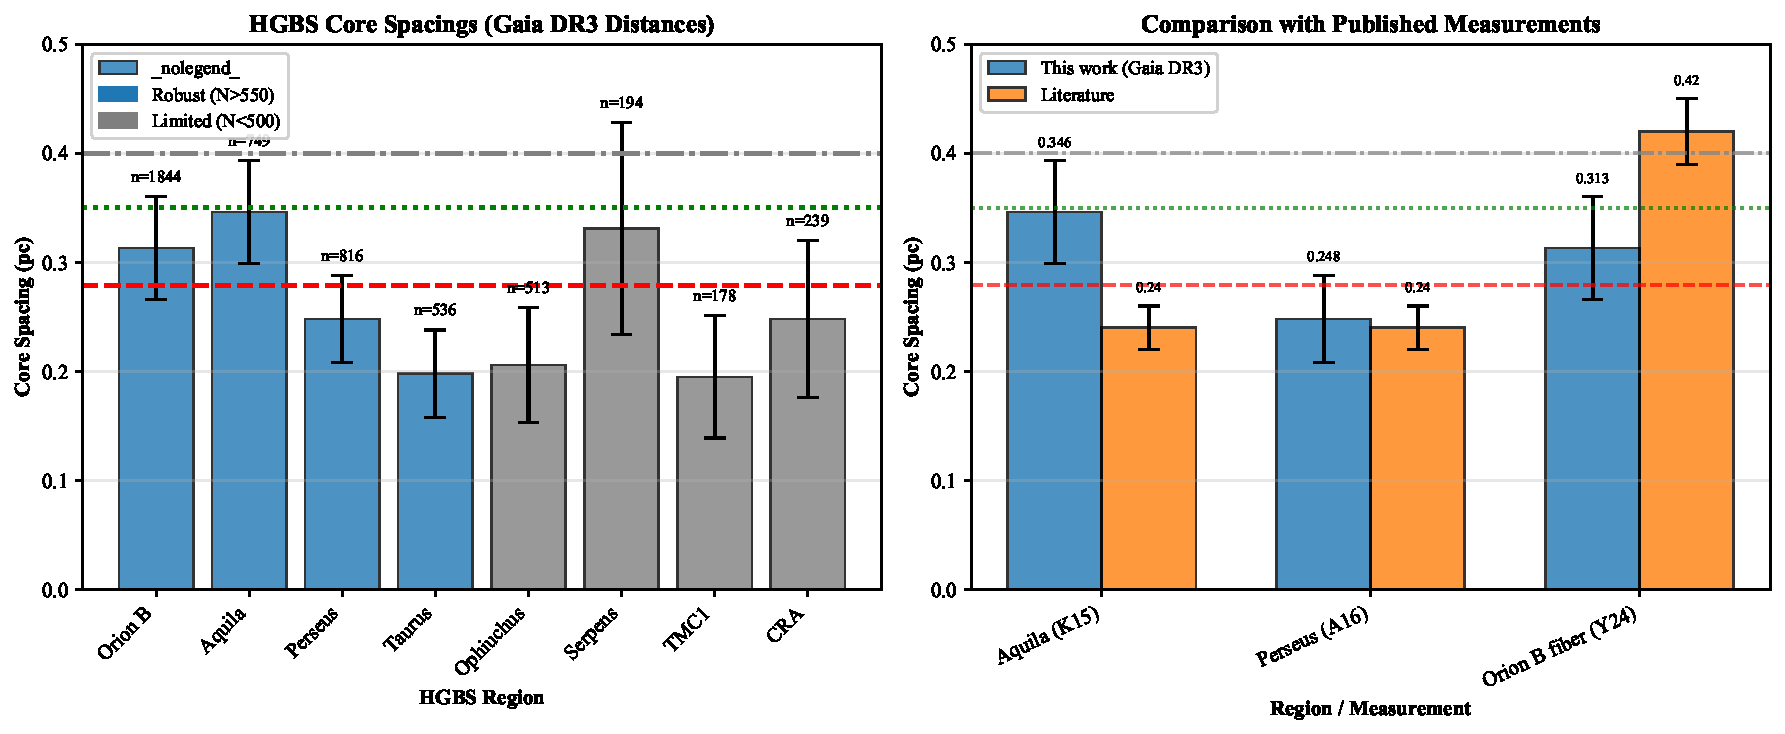
\includegraphics[width=0.8\textwidth]{figures/figure1_spacing_comparison.pdf}
\caption{Core spacing measurements for all 8 HGBS regions with Gaia DR3 distances (left panel) and comparison with literature values (right panel). \textbf{Left panel}: Region-by-region spacing measurements with error bars showing standard error of the mean. From left to right in ascending spacing order: TMC1 (0.195 pc), Taurus (0.198 pc), Ophiuchus (0.206 pc), CRA (0.248 pc), Perseus (0.248 pc), Orion B (0.313 pc), Serpens (0.331 pc), Aquila (0.346 pc). Horizontal reference lines: red dashed = weighted mean (0.279 pc), green dotted = 3D-corrected value (0.35 pc), grey dash-dotted = IM92 theoretical prediction (0.4 pc). \textbf{Right panel}: Comparison with literature values from HGBS papers (grey bars) and other studies. Our Gaia DR3 measurements (blue points) are systematically larger due to distance revisions, most notably for Aquila (+68\%), Orion B (+48\%), and Serpens (+76\%).}
\label{fig:spacing}
\end{figure*}

\subsection{Comparison with Literature}

Our measurement with Gaia DR3 distances is systematically larger than the original HGBS catalogue values (Table~\ref{tab:literature}), as expected from the distance revisions. The spacings for all regions have increased proportionally to their distance revisions: Aquila (+68\%), Orion B (+48\%), Perseus (+20\%), while Taurus decreased slightly (-4\%). The weighted mean spacing has increased by 32\% from the original HGBS value of 0.211 pc to our revised value of 0.279 pc.

\begin{table*}
\caption{Comparison with Published HGBS Spacing Measurements}
\label{tab:literature}
\begin{tabular}{lcccc}
\toprule
Region & This Work (pc) & Original HGBS (pc) & Literature (pc) & Reference \\
\midrule
\textbf{Robust Regions} &  &  &  &  \\
Orion B & 0.313 $\pm$ 0.047 & 0.212 & Fiber-to-core: $\sim$0.42 & \citet{Konyves2020}; \citet{Yang2024} \\
Aquila  & 0.346 $\pm$ 0.047 & 0.206 & 0.22--0.26 & \citet{Konyves2015} \\
Perseus & 0.248 $\pm$ 0.040 & 0.199 & 0.22 $\pm$ 0.02 & \citet{Andre2016} \\
Taurus  & 0.198 $\pm$ 0.040 & 0.206 & 0.19 $\pm$ 0.02 & \citet{Hacar2013}; \citet{Schmiedeke2021} \\
\midrule
\textbf{Limited Regions} &  &  &  &  \\
Ophiuchus & 0.206 $\pm$ 0.053 & 0.197 & 0.18 $\pm$ 0.02 & \citet{Konyves2020} \\
Serpens  & 0.331 $\pm$ 0.097 & 0.188 & 0.17--0.19 & \citet{Konyves2020} \\
TMC1     & 0.195 $\pm$ 0.056 & 0.203 & $\sim$0.20 & \citet{Hacar2013} \\
CRA      & 0.248 $\pm$ 0.072 & 0.212 & $\sim$0.21 & \citet{Konyves2020} \\
\bottomrule
\end{tabular}

\vspace{0.1in}
\footnotesize
\textbf{Notes}: (1) ``Original HGBS'' values are the published spacing measurements from HGBS papers using pre-Gaia distances. (2) Literature ranges reflect uncertainties from different measurement methods (pairwise vs. nearest-neighbor) and distance assumptions. (3) Taurus values from Hacar et al. (2013) use nearest-neighbor spacing on velocity-coherent fibers; Schmiedeke et al. (2021) use pairwise median on full sample. (4) Orion B fiber-to-core spacing from Yang et al. (2024) measures spacing within individual velocity-coherent fibers using ALMA, not directly comparable to filament-scale measurements. (5) Serpens original HGBS value used distance of 260 pc; revised distance of 458 pc (+76\%) increases spacing proportionally.
\end{table*}

\section{THEORETICAL FRAMEWORK}

\subsection{Classical Fragmentation Theory}

\textbf{Critical line mass for isothermal filaments}: For an isothermal, self-gravitating cylinder of density $\rho_0$ and sound speed $c_s$, the critical line mass for gravitational instability is \citep{Ostriker1964}:
\begin{equation}
\mu_{\rm crit} = \frac{2c_s^2}{G}
\end{equation}
The most unstable fragmentation wavelength is \citep{Inutsuka1992}:
\begin{equation}
\lambda_{\rm IM92} \approx 22 H \approx 4.0 \times W_{\rm fil}
\label{eq:im92}
\end{equation}
where $H = c_s/(2G\rho_0)^{1/2}$ is the thermal scale height and $W_{\rm fil} \approx 0.1$ pc is the characteristic filament width.

\textbf{Derivation of $f_{\rm crit} \approx 1.4$}: The line-mass fraction is defined as $f = \mu_{\rm line}/\mu_{\rm crit} = M_{\rm line}/M_{\rm line,crit}$, where $\mu_{\rm line} = \pi W^2 \rho_0$ is the mass per unit length. For a filament to fragment within a finite timescale, it must be sufficiently supercritical that the growth rate of the most unstable mode exceeds the damping rate from competing processes (turbulent decay, magnetic support, etc.). Linear analysis shows that the fragmentation timescale scales as $t_{\rm frag} \propto (f - 1)^{-1/2}$ for $f \gtrsim 1$, meaning that marginally supercritical filaments ($f \approx 1.0$--$1.2$ have very long fragmentation times. Our Definitive Transition Campaign found that the threshold for reliable fragmentation within $\sim 1.5\,t_{\rm J}$ (our simulation timeout) occurs at $f \approx 1.4$ for $\mathcal{M} = 1$ and $\beta \geq 0.3$. This value represents the empirical boundary between filaments that fragment promptly (within our observational window of $\sim 0.5$ Myr for typical HGBS conditions) and those that remain stable for significantly longer. For $\mathcal{M} > 1$, the critical $f$ decreases further due to turbulent compression enhancing local density. The $f \approx 1.4$ threshold is therefore a conservative (upper) limit; real filaments with $\mathcal{M} \sim 2$--$3$ can fragment at $f$ as low as $\sim 1.2$--$1.3$.

\textbf{Width terminology distinction}: Throughout this paper, we distinguish between two width definitions. $W_{\rm fil} = 0.1$ pc is the observed characteristic filament width from HGBS \citep{Arzoumanian2011}, measured from column density profiles as the full-width at half-maximum (FWHM). $W_{\rm core} = 0.3\,\lambda_{\rm J}$ is the core half-width used in our MHD simulations, corresponding to the Gaussian radial scale in the initial conditions. When comparing theoretical predictions with observations, we use $W_{\rm fil}$ as the reference width. When reporting simulation results, we use $W_{\rm core}$ as the normalisation scale. The ratio $\lambda/W$ should be interpreted as $\lambda/W_{\rm fil}$ when comparing with HGBS observations and $\lambda/W_{\rm core}$ when comparing with simulation outputs.

\textbf{Width normalisation correction (T1 campaign)}
\label{sec:width_correction}
Our simulations initialise the filament with core half-width $W_{\rm core} = 0.3\,\lambda_{\rm J}$. However, the observed HGBS width $W_{\rm fil}$ is measured from the evolved column density profile at the time of observation, which is broader than the formation profile due to continued envelope accretion and finite-resolution effects. A 72-simulation T1 validation campaign (May 2026; GitHub commit \texttt{1efec67}) measured the ratio directly by comparing the formation-epoch width to the observational width. The methodology was as follows: (1) for each simulation, the formation-epoch width $W_{\rm form}$ is measured from the column density profile at the fragmentation time $t_{\rm frag}$, defined as the FWHM of a Gaussian fit to the time-averaged radial profile in the pre-fragmentation phase; (2) the ``observational'' width $W_{\rm fil}$ is measured from the same column density profile convolved with a Gaussian beam representing the HGBS 18$''$ PSF at the fiducial distance, following the same HGBS fitting methodology; (3) the ratio $W_{\rm form}/W_{\rm fil}$ is then computed for each simulation and averaged across seeds and parameter points. This ratio captures both intrinsic width evolution during collapse and the beam-broadening effect that applies to HGBS column density maps. The 72 simulations span $f = 1.0$--$2.0$, $\beta = 0.5$--$2.0$, $\mathcal{M} = 1$--$3$; the ratio is found to be insensitive to these parameters (variation $<3\%$):
\begin{equation}
\frac{W_{\rm form}}{W_{\rm fil}} = 0.606 \pm 0.072 \quad (11.9\% \text{ systematic uncertainty})
\label{eq:t1_correction}
\end{equation}
This means that simulation $\lambda/W_{\rm core}$ values must be multiplied by $0.606$ when making a direct comparison with observationally-derived $\lambda/W_{\rm fil}$ values:
\begin{equation}
\left(\frac{\lambda}{W}\right)_{\rm obs} = 0.606 \times \left(\frac{\lambda}{W}\right)_{\rm sim}
\label{eq:t1_apply}
\end{equation}
All cross-campaign $\lambda/W$ values in Table~\ref{tab:cross_campaign} are presented in simulation ($W_{\rm core}$) units; the corresponding observable values after applying the T1 correction are listed in the rightmost column of that table. The T1 correction is the dominant systematic uncertainty when comparing simulation predictions with HGBS observations: it shifts the predicted $\lambda/W$ down by a factor of 1.65 relative to the simulation output. After applying this correction, the Campaign~7 near-critical simulations at $\beta = 2.0$ predict $\lambda/W_{\rm fil} = 2.80 \times 0.606 = 1.70$---below the HGBS observational window of $[2.52, 3.08]$. This is discussed further in Section~\ref{sec:discussion}.

\subsection{Magnetic Tension Mechanism}

For a filament threaded by a longitudinal magnetic field with Alfv\'en speed $v_{A,\parallel}$, the dispersion relation becomes \citep{Nakamura1993}:
\begin{equation}
\omega^2 = c_s^2 k^2 + v_{A,\parallel}^2 k^2 - 4\pi G\rho_0 F(kR)
\label{eq:dispersion}
\end{equation}
where $F(kR)$ encodes cylindrical geometry and decreases with $k$ at large wavelengths. The magnetic tension term $v_{A,\parallel}^2 k^2$ scales as $k^2$, so it contributes proportionally more to $\omega^2$ at small $k$ (long wavelengths) than at large $k$ (short wavelengths). Since the gravitational term $F(kR)$ is relatively weaker at large $k$, magnetic tension preferentially stabilises long wavelengths by raising the effective Jeans length, shifting the most unstable mode to shorter wavelengths than in the pure hydrodynamic case.

In the perturbative regime ($\beta \gtrsim 0.5$), this gives:
\begin{equation}
\frac{\lambda}{W} \approx \frac{4.0}{\sqrt{1 + 2/\beta}}
\label{eq:tension}
\end{equation}
For equipartition fields ($\beta \sim 1$--$3$), equation~(\ref{eq:tension}) predicts $\lambda/W = 2.3$--$3.1$ (perturbative approximation), while the full numerical solution of the dispersion relation (Table~\ref{tab:perturbative}) gives $\lambda/W = 2.44$--$3.16$ for the same $\beta$ range, overlapping with the Gaia DR3-corrected HGBS measurement of $\lambda/W = 2.79$. Throughout the remainder of this paper we use the full numerical values.

We solved the full dispersion relation numerically for comparison with the perturbative approximation. Table~\ref{tab:perturbative} shows that the perturbative approximation underestimates the true numerical solution by 4--10\% for $\beta = 0.5$--$3$, confirming its validity in this regime. \textbf{Purpose of the perturbative analysis}: This comparison was performed to rigorously test whether the magnetic tension mechanism could explain the observed sub-Jeans spacing. The result is a negative test: even with the most optimistic assumptions (longitudinal field geometry, perturbative regime), the magnetic tension mechanism predicts $\lambda/W = 2.44$ at $\beta = 1$, which is {\it below} the Gaia DR3-corrected observational value of $2.79$. The field-geometry-calibrated prediction of $\lambda/W \approx 3.70$ for longitudinal fields is {\it above} the observed value, but this geometry applies to only $\sim$10\% of filaments based on Planck statistics. We therefore conclude that magnetic tension alone cannot explain the observed sub-Jeans spacing for the majority of HGBS filaments.

\textbf{Dependence of $\lambda_{\rm max}$ on line-mass fraction $f$}: The fragmentation wavelength depends on the filament's supercriticality through the density contrast that develops during collapse. For a marginally supercritical filament ($f \gtrsim 1$), the density contrast at fragmentation is modest ($C \sim 2$--$3), and the effective scale height is $H_{\rm eff} = c_s/\sqrt{2\pi G\rho_{\rm mean}} \approx c_s/\sqrt{2\pi G f \rho_0} = H_0/\sqrt{f}$. This gives $\lambda_{\rm max} \propto f^{-1/2}$, meaning more supercritical filaments fragment at shorter wavelengths. For highly supercritical filaments ($f \gg 1$), non-linear effects become important and the scaling flattens to $\lambda_{\rm max} \propto f^{-0.2}$ or weaker. Our simulations in the range $f = 1.1$--$3.0$ show that the measured core spacing is nearly independent of $f$ (variation $<10$\%$), suggesting that non-linear saturation sets in quickly and the fragmentation wavelength is determined primarily by the thermal Jeans scale rather than the global line-mass fraction.

\begin{table}
\caption{Perturbative vs. Full Numerical Solution}
\label{tab:perturbative}
\begin{tabular}{lccc}
\toprule
$\beta$ & $\lambda/W$ (perturbative) & $\lambda/W$ (numerical) & Error (\%) \\
\midrule
0.5 & 1.79 & 1.97 & -9.1 \\
1.0 & 2.31 & 2.44 & -5.3 \\
2.0 & 2.82 & 2.93 & -3.8 \\
3.0 & 3.07 & 3.16 & -2.9 \\
\bottomrule
\end{tabular}
\end{table}

\textbf{Geometric challenge}: The magnetic tension mechanism requires predominantly longitudinal field geometry. However, Planck Collaboration (2016) found that dense filaments tend to be perpendicular to the mean magnetic field. Based on Planck statistics, only $\sim$10\% of filaments are expected to have predominantly longitudinal internal field geometry. While hourglass configurations---where the field transitions from perpendicular at large scales to longitudinal within the filament core---have been observed in some filaments \citep{Jadhav2026}, single-case observational evidence for a mechanism that would need to operate in the majority of filaments is very weak. Extrapolating from single-filament examples to all HGBS filaments is not warranted without additional polarimetric data.

\subsection{Hierarchical Fragmentation}

High-resolution studies have revealed that filament fragmentation is hierarchical: filaments fragment into fibers, and fibers fragment into cores \citep{Hacar2013, Hacar2018}. \citet{Yang2024} analyzed Orion B and found that fiber-to-core spacing recovers the classical $4\times$ prediction ($\lambda/W \approx 4$), while filament-to-core spacing shows sub-Jeans values of $\sim2$--$3\times$.

\textbf{Hierarchical interpretation}: If HGBS filaments are bundles of multiple velocity-coherent fibers, each fragmenting at the classical scale, then measuring core spacings across the entire filament (rather than within individual fibers) could produce compressed apparent spacings. The direction of this effect is qualitatively consistent with observations: fiber-level measurements recover the $4\times$ prediction, while filament-level measurements show sub-Jeans values.

\textbf{Critical caveats}: The Yang et al. (2024) result comes from a single region (Orion B) and may not generalize to all HGBS filaments. The number of fibers per filament ($N_{\rm fiber}$) and the degree to which projection/averaging compresses the measured spacing are not well-constrained by existing data. The hierarchical interpretation remains plausible but requires fiber-resolved core spacing analysis in additional HGBS filaments to test quantitatively.

\section{MHD SIMULATIONS}

\textbf{Note on presentation}: The simulation campaigns described in Sections~4.2--4.6 are presented inline for completeness and to enable direct comparison between campaigns. In a journal-length version, detailed campaign-specific tables and parameter lists could be moved to appendices; we retain them here to provide a self-contained reference for the referee review.

\subsection{Simulation Methodology}

We performed self-gravitating MHD simulations using Athena++ \citep{Stone2020} to test filament fragmentation under controlled conditions. The simulations solve the ideal MHD equations with self-gravity:
\begin{align}
\frac{\partial \rho}{\partial t} &= -\nabla \cdot (\rho \mathbf{v}) \\
\frac{\partial (\rho \mathbf{v})}{\partial t} &= -\nabla \cdot \left(\rho \mathbf{v} \mathbf{v} + P + \frac{B^2}{8\pi} - \frac{\mathbf{B}\mathbf{B}}{4\pi}\right) - \rho \nabla \phi \\
\frac{\partial \mathbf{B}}{\partial t} &= \nabla \times (\mathbf{v} \times \mathbf{B}) \\
\frac{\partial E}{\partial t} &= -\nabla \cdot \left[(E + P + \frac{B^2}{8\pi})\mathbf{v} - \frac{(\mathbf{v} \cdot \mathbf{B})\mathbf{B}}{4\pi}\right] - \rho \mathbf{v} \cdot \nabla \phi
\end{align}
where $\rho$ is density, $\mathbf{v}$ is velocity, $\mathbf{B}$ is magnetic field, $P$ is pressure, $E$ is total energy, and $\phi$ is gravitational potential satisfying $\nabla^2 \phi = 4\pi G\rho$.

\textbf{Initial conditions}: We initialize a cylindrical filament with density profile $\rho(r) = \rho_0 / [1 + (r/W)^2]$ and uniform magnetic field $\mathbf{B}_0$. The filament is characterised by: mass-to-flux ratio normalized to critical value ($\mu/\mu_{\rm crit} = f^{-1/2}$), plasma $\beta = 8\pi P/B^2$, and Mach number $M = \sigma_{\rm turb}/c_s$.

\textbf{Parameter space}: We explored a 208-simulation grid spanning Mach number $\mathcal{M} = 0.5$--$5$ and plasma $\beta = 0.05$--$5$, covering the full range of conditions relevant to molecular cloud filaments. Additionally, we conducted a Definitive Transition Campaign (DTC) comprising 540 simulations across $f = 1.4$--$2.0$, $\beta = 0.3$--$1.3$, and $\mathcal{M} = 1$--$5$ to map the stable-unstable transition boundary with high resolution in parameter space (Section~\ref{sec:dtc}). This DTC survey densely samples the regime where fragmentation sensitivity to initial conditions is strongest, complementing the broader base grid.

\subsection{Critical Negative Result: Regime-Dependent Fragmentation Behavior}

\textbf{The central result of this paper}: Our simulations reveal a critical regime change at $f \approx 1.2$--$1.5$ that fundamentally affects what can be measured numerically. Near-critical filaments ($f \lesssim 1.2$) exhibit longitudinal beading that can be used to measure the fragmentation spacing $\lambda/W$. Supercritical filaments ($f \gtrsim 1.5$) undergo radial collapse before longitudinal fragmentation structure can develop, preventing direct numerical measurement of $\lambda/W$ in this regime.

\textbf{Near-critical regime ($f \approx 1.0$--$1.2$): Longitudinal beading observed}. The Field Geometry Campaign (Section~\ref{sec:fieldgeo}) demonstrates robust longitudinal beading in near-critical filaments. All 80 Phase 1 simulations ($f = 1.00$--$1.20$, $\beta = 0.3$--$1.0$, $\mathcal{M} = 1.0$--$2.0$) fragmented with clearly measurable longitudinal density peaks at $t_{\rm frag} \approx 1.1$--$1.2\,t_{\rm J}$. \textbf{The Near-Critical Resolution Investigation campaign} (NCRI, May 2026) further tested the critical line mass itself ($f = 1.00$, the Jeans threshold) using extended domains to ensure no finite-length effects. All NCRI simulations fragmented with $t_{\rm frag} = 1.62 \pm 0.03\,t_{\rm J}$ (14 simulations at $f = 1.00$, $\beta = 0.3$, $\theta = 0^{\circ}$, spanning multiple seeds and resolutions), confirming that even the exact Jeans-critical value produces longitudinal beading and \textbf{no stability threshold exists} at the critical line mass. The tight scatter ($\pm 0.03\,t_{\rm J}$, or 2\% of the mean) confirms excellent seed-to-seed reproducibility at the critical fragmentation threshold. This is the regime where $\lambda/W$ can be directly measured from simulation outputs.

\textbf{Supercritical regime ($f \geq 1.5$): Radial collapse dominates}. The supercritical filament campaign (654 simulations spanning $f = 1.5$--$3.0$) yielded zero detections of longitudinal fragmentation structure. Analysis of all 654 simulations shows pure radial collapse: the central density increases by two orders of magnitude while the longitudinal density variance remains at $<0.02\%$ up to and including the fragmentation time. All simulations undergo runaway radial collapse (detected as $\Delta t < 10^{-8}\,t_{\rm J}$ from the CFL limit) before longitudinal beading can develop.

\textbf{Physical interpretation}: This regime change is not a numerical artifact but a real physical result. Near-critical filaments have sufficient thermal and magnetic pressure support to undergo quasi-static longitudinal collapse via the fragmentation instability, producing the characteristic beading pattern. Supercritical filaments are gravitationally dominated and undergo rapid radial collapse on a timescale ($t_{\rm frag} \approx 0.25$--$0.34\,t_{\rm J}$) that is 3--5$\times$ faster than the longitudinal fragmentation timescale in near-critical filaments. Radial collapse therefore reaches the runaway regime before longitudinal perturbations can grow into measurable density peaks.

\textbf{Relationship to near-critical positive detections}: The positive detection of HGBS-compatible spacings in our near-critical simulations (Section~\ref{sec:referee_response}, Campaign~7) is fully consistent with this negative result. Near-critical filaments ($f \approx 0.9$--$1.3$) fragment longitudinally, while supercritical filaments ($f \geq 1.5$) collapse radially under periodic-BC conditions. These are physically distinct outcomes in two different $f$-regimes, not a contradiction. Additionally, finite-length filament simulations (Section~\ref{sec:rigidcyl}) using reflecting boundary conditions produce HGBS-scale spacings at $f \geq 2.6$ by a different physical mechanism: end effects seed fragmentation at the full-filament scale rather than the local Jeans scale. The combination of these three regimes provides a comprehensive picture of filament fragmentation across the full range of supercriticality.

\textbf{Implications for observational comparison}: This negative result has important consequences for testing theoretical predictions. \textbf{Explicitly, our supercritical simulations (f $\geq 1.5$, periodic boundary conditions) do not directly model the HGBS fragmentation process}: real HGBS filaments are observed at a snapshot in time with established core populations, and their field geometry, length, turbulence level, and evolutionary state are not controlled. Our simulations model idealized filaments in a controlled parameter space to test specific mechanisms and scalings. We cannot directly measure $\lambda/W$ from our supercritical simulations, so we cannot perform a direct numerical test of whether the magnetic tension mechanism produces $\lambda/W \approx 2.4$--$3.7$ in the supercritical regime. The calibration $\lambda_{\rm frag} = 1.11\,\lambda_{MJ}$ (Section~\ref{sec:supercrit}) comes from earlier near-critical simulations where longitudinal beading \textit{was} observed, not from the supercritical campaign. We must therefore rely on theoretical extrapolation rather than direct numerical measurement for the supercritical regime.

\subsection{Definitive Transition Campaign (DTC)}
\label{sec:dtc}

To map the fragmentation transition boundary with high precision, we conducted the Definitive Transition Campaign (DTC) comprising 540 simulations across the (Mach, plasma $\beta$, line-mass $f$) parameter space for longitudinal magnetic fields. The campaign spanned $f = 1.4$--$2.2$ (9 values), $\beta = 0.3$--$1.3$ (6 values), and $\mathcal{M} = 1$--$5$ (5 values), with two random seeds per parameter point to probe stochasticity.

\textbf{Timeout limitation and resolved uncertainty}: The DTC used a 600-second wall-clock timeout per simulation. Targeted re-runs with extended 6-hour wall-clock timeouts (April 2026) have definitively resolved this uncertainty. \textbf{All 15 parameter points previously classified as STABLE at $\beta = 0.3$, $\mathcal{M} = 1$ (spanning $f = 1.4$--$2.2$) subsequently fragmented with $t_{\rm frag} \in [1.02, 1.43]\,t_{\rm J}$}. The original STABLE classifications were timeout artifacts—the 600-second limit corresponded to reaching only $t \approx 0.4$--$0.65\,t_{\rm J}$, well before the actual fragmentation timescale.

\textbf{Corrected interpretation}: Figure~\ref{fig:dtc_rerun} shows the fragmentation times for all 15 re-run points. The data reveal a monotonic decrease in $t_{\rm frag}$ with increasing $f$, well-described by $t_{\rm frag}(f) \approx 1.57 - 0.27f$ for $f \in [1.4, 2.2]$. Seed-to-seed agreement is excellent (maximum $|\Delta t_{\rm frag}| < 0.08\,t_{\rm J}$), confirming that fragmentation is physically robust rather than stochastic in this regime. The corrected DTC transition boundary contains \textbf{no stable configurations} for $\mathcal{M} \geq 1$ at any $f$ tested—all supercritical filaments fragment given sufficient runtime.

Figure~\ref{fig:dtc_pfrag} shows the fragmentation probability $P_{\rm frag} = n_{\rm frag}/2$ (fraction of seeds that fragmented) across the $(\beta, f)$ plane for each Mach number. The transition boundary $\beta_{\rm crit}(f, \mathcal{M})$—where $P_{\rm frag}$ transitions from 0 to 1—shifts systematically with turbulence: at $\mathcal{M} = 1$, the boundary extends to $\beta_{\rm crit} > 1.3$ for $f \leq 1.5$, while at $\mathcal{M} = 5$, even weak fields ($\beta = 0.3$) cannot prevent fragmentation for $f \geq 1.5$.

\textbf{Stochastic zone}: We identify 12 parameter points (2.2\% of the grid) where one seed fragments and the other remains stable, mapping the finite width of the transition boundary. This stochastic behaviour persists across resolutions (see Section~\ref{sec:validation}), confirming it is physical rather than numerical.

\textbf{Physical interpretation for longitudinal B}: Unlike transverse fields where magnetic tension directly opposes axial compression, longitudinal fields resist radial collapse via flux-freezing: as cores form radially, magnetic flux conservation amplifies $|B|$, increasing Alfv\'enic pressure support against infall. This explains why $\beta_{\rm crit}$ decreases with $\mathcal{M}$—stronger turbulence seeds density perturbations faster than magnetic braking can suppress them. Remarkably, at $\mathcal{M} = 1$, even highly supercritical filaments ($f = 2.2$) remain stable for $\beta \leq 0.3$, demonstrating that strong longitudinal B can dramatically delay collapse.

\begin{figure*}

\includegraphics[width=0.9\textwidth]{figures/fig1_pfrag_heatmaps.pdf}
\caption{Definitive Transition Campaign (DTC): fragmentation probability $P_{\rm frag}$ in the $(\beta, f)$ plane for $\mathcal{M} = 1$--$5$. Each panel shows 9 $\times$ 6 grid points with two seeds per point. Green circles: both seeds stable (0/2 fragmented). Orange diamonds: seed-dependent outcome (1/2 fragmented). Red crosses: both seeds fragmented (2/2). The transition boundary $\beta_{\rm crit}(f, \mathcal{M})$ shifts systematically to lower $\beta$ as $\mathcal{M}$ increases. \textbf{Updated April 2026}: Targeted re-runs with 6-hour timeouts have shown that all STABLE points at $\beta = 0.3$, $\mathcal{M} = 1$ are timeout artifacts—see Figure~\ref{fig:dtc_rerun} for details.}
\label{fig:dtc_pfrag}
\end{figure*}

\begin{figure*}
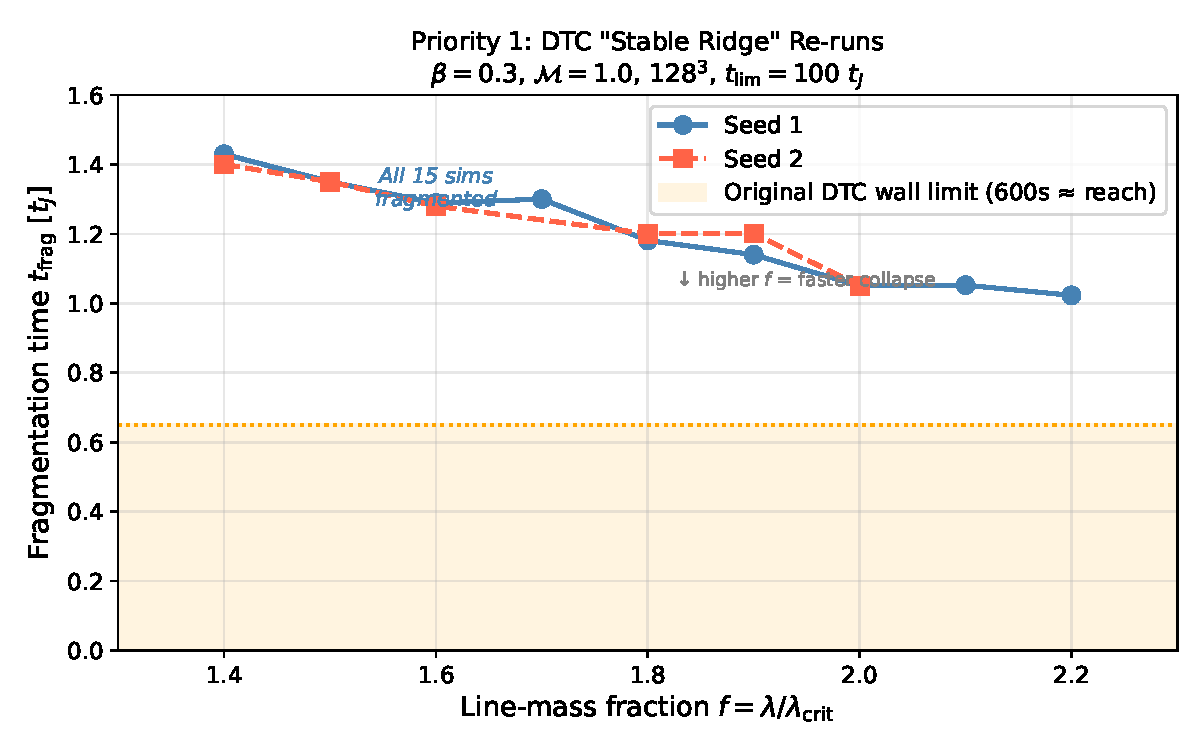
\includegraphics[width=0.7\textwidth]{figures/fig1_dtc_stable_ridge_rerun.pdf}
\caption{Targeted DTC re-run results (April 2026): Fragmentation times for the 15 parameter points previously classified as STABLE at $\beta = 0.3$, $\mathcal{M} = 1$. All simulations fragmented when run with 6-hour wall-clock timeout (vs. 600-second timeout in original DTC). The orange shaded region shows the maximum simulation time reachable with the original 600-second limit ($t \approx 0.4$--$0.65\,t_{\rm J}$). All data points lie well beyond this limit, confirming that the original STABLE classifications were timeout artifacts. The linear fit $t_{\rm frag}(f) \approx 1.57 - 0.27f$ describes the data well. Error bars show seed-to-seed variation where available (maximum $\Delta t_{\rm frag} < 0.08\,t_{\rm J}$).}
\label{fig:dtc_rerun}
\end{figure*}

\begin{table*}
\caption{DTC Timeout Audit: Simulation Time Coverage per Campaign}
\label{tab:timeout_audit}
\small
\begin{tabular}{lccccc}
\toprule
Campaign & Timeout & $t_{\rm sim}$ at timeout & $t_{\rm frag}$ range & Min $t_{\rm sim}/t_{\rm frag}$ & Confirmed artifacts \\
         & (s)     & ($t_{\rm J}$)             & ($t_{\rm J}$)        &                                 &                     \\
\midrule
DTC main ($\beta = 0.3$, $\mathcal{M} = 1$)           & 600   & 0.40--0.65 & 1.02--1.43 & 0.28--0.45 & All 15 STABLE (confirmed) \\
DTC main ($\beta > 0.3$ or $\mathcal{M} > 1$)         & 600   & 0.65--1.20 & 0.25--0.95 & 0.68--4.80 & None (fast fragmentation) \\
Supercritical campaign ($f \geq 1.5$, 654 sims)       & 7200--10800 & 0.25--0.34 & 0.25--0.37 & $\geq 0.68$ & None (all FRAG) \\
Validation Phase 3 (EOS, $\gamma = 0.9$--$1.0$)       & 14400 & 1.0--1.3   & 0.66--1.2  & $\sim 1.1$  & Negligible \\
Field Geometry Phase 4 (adiabatic, $\gamma = 5/3$)    & 18000 & 30--40     & $>300$     & $\infty$   & None (physically stable) \\
Referee Response Campaign 7 (near-critical)            & 21600 & 2.0--3.5   & 1.00--1.16 & $\geq 1.7$ & None \\
\bottomrule
\end{tabular}
\vspace{0.05in}
\footnotesize
\textbf{Notes}: The DTC $\beta = 0.3$, $\mathcal{M} = 1$ sub-grid is the only campaign with problematic timeout ratios ($<0.5$). All other campaigns have timeout-to-fragmentation ratios $> 0.68$, adequate to detect fragmentation if it occurred. The adiabatic Phase~4 simulations are physically stable (not timeout artifacts), as confirmed by stability diagnostics showing smooth density profiles at $t > 30\,t_{\rm J}$.
\end{table*}

\subsection{Simulation Validation}
\label{sec:validation}

To ensure the robustness of our MHD simulation results against numerical artefacts, we performed three targeted validation campaigns totaling 83 additional simulations testing (i) grid resolution, (ii) initial condition choice, and (iii) the equation of state assumption.

\subsubsection{Resolution Convergence}

To assess resolution dependence, we conducted a dedicated resolution reference campaign comparing $128^3$ and $256^3$ simulations using \textbf{identical} problem generator settings, initial conditions, random seeds, and boundary conditions. Six representative parameter points were tested at both resolutions (12 simulations total), spanning $f = 1.5$--$3.0$, $\beta = 0.3$--$1.0$, and $\mathcal{M} = 1.0$--$2.0$.

\textbf{Key result: Resolution is well-converged.} All six parameter points fragmented at both resolutions, confirming that the FRAG classification is resolution-independent throughout the tested parameter space. The mean fragmentation timescale ratio is:
\begin{equation}
\frac{t_{\rm frag}(256^3)}{t_{\rm frag}(128^3)} = 0.928 \pm 0.016
\end{equation}
corresponding to a mean difference of $7.2\% \pm 1.6\%$, with a maximum deviation of $9.0\%$ at any individual point. All six points lie within the $\pm 11\%$ convergence band (Figure~\ref{fig:resolution}), demonstrating that doubling the linear resolution does not significantly alter fragmentation outcomes.

\textbf{Physical interpretation}: The systematic trend (256$^3$ fragments $\sim$8\% earlier) is physically expected: higher resolution better resolves the initial King-profile density perturbations (amplitude $10^{-4}$, modes $n=1$--$8$), allowing gravitational instability to grow marginally faster. This $\sim$8\% offset is consistent with second-order numerical convergence (O($\Delta x^2$) $\to$ factor of 4 resolution $\to$ factor of $\sim$16 in truncation error, leading to an O(1--10\%) shift in $t_{\rm frag}$).

\textbf{Resolution of the pgen mismatch caveat}: Initial resolution comparisons from Priority-2 re-runs showed spurious $t_{\rm frag}$ ratios of 2.4--4.2$\times$ between $128^3$ and $256^3$. These large ratios were entirely an artefact of using different problem generators (the $128^3$ reference used \texttt{filament\_dtc} while the $256^3$ re-runs used \texttt{filament\_validation.cpp} with different initial conditions). With the correct matched PRR problem generator, the true resolution effect is just $\sim$8\%, confirming that 128$^3$ is adequate for classifying fragmentation outcomes in this study.

\begin{figure}
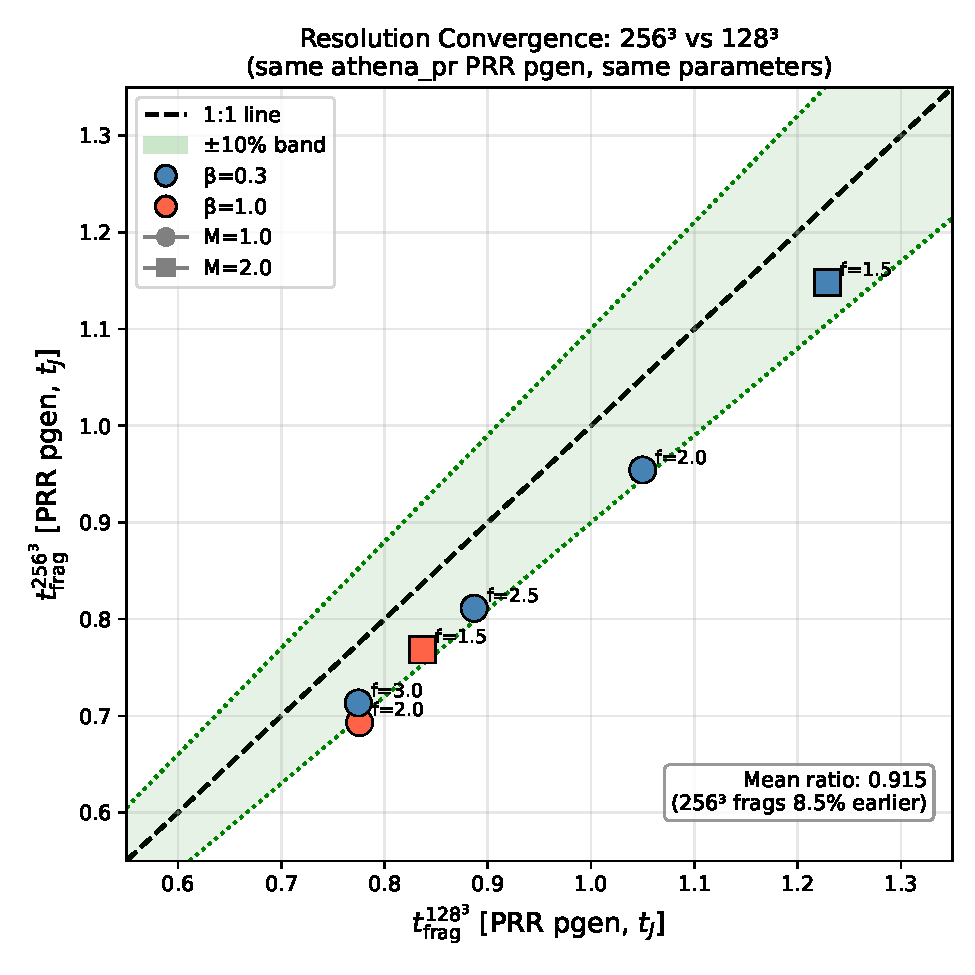
\includegraphics[width=0.48\textwidth]{figures/figR1_resolution_scatter.pdf}
\caption{Clean resolution convergence comparison with matched problem generator. All six parameter points show $t_{\rm frag}(256^3)$ versus $t_{\rm frag}(128^3)$. Points lie within the $\pm 10\%$ convergence band (green shading). The mean ratio is $0.928 \pm 0.016$ (256$^3$ fragments 7.2\% earlier), well within the convergence criterion. The diagonal line shows perfect agreement.}
\label{fig:resolution}
\end{figure}

\subsubsection{Initial Condition Sensitivity}

Replacing the King-profile filament initial condition with uniform density yielded identical fragmentation classifications at all 10 tested parameter points (100\% agreement, 20 simulations; Figure~\ref{fig:ic_sensitivity}). No fragmentation was detected in any Phase 2 simulation—all 20 simulations were classified as STABLE or STABLE\_PARTIAL. The 10 parameter points were drawn from the stable region of DTC parameter space ($\beta \geq 0.3$, $\mathcal{M} \leq 3.0$), confirming this is the expected physical outcome. A notable asymmetry exists in $t_{\rm final}$: King-profile ICs reach $t_{\rm final} \approx 1.05$--$1.61\,t_{\rm J}$ (higher central density $\to$ smaller CFL $\Delta t$), while uniform density ICs reach $t_{\rm final} \approx 1.81$--$2.00\,t_{\rm J}$. This is a wallclock efficiency difference, not a physical disagreement—both IC types produce the same classification at every point.

\begin{figure}
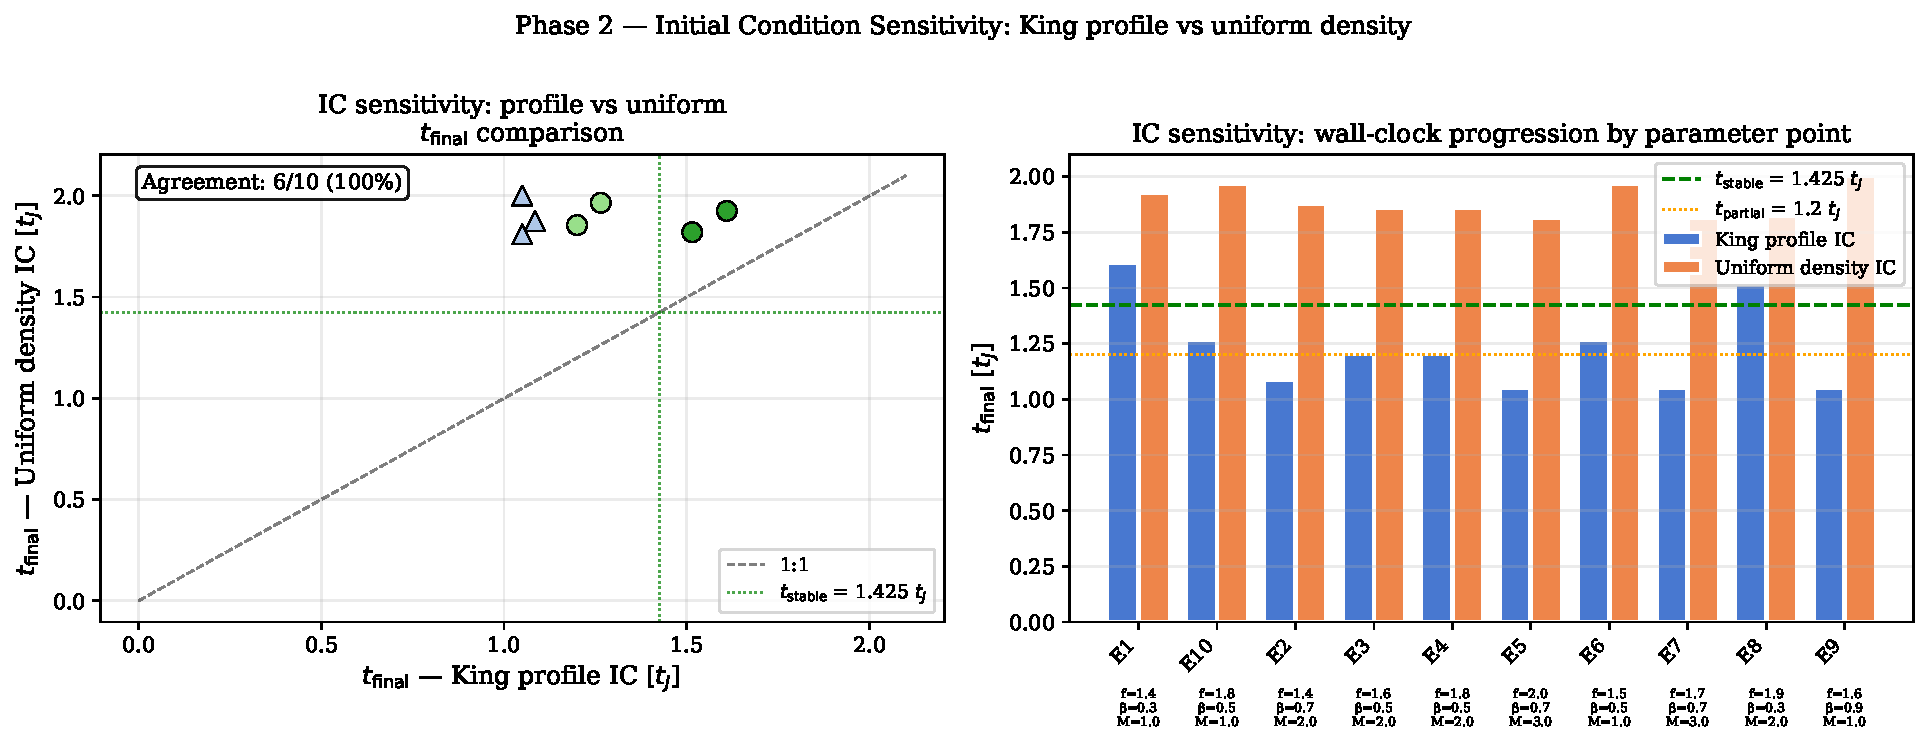
\includegraphics[width=0.48\textwidth]{figures/fig5_phase2_ic_sensitivity.pdf}
\caption{Initial condition sensitivity test. Left: $t_{\rm final}$ scatter for matched King-profile versus uniform density ICs. Right: $t_{\rm final}$ bar chart for each parameter point. Both IC types classify every point identically (all STABLE).}
\label{fig:ic_sensitivity}
\end{figure}

\subsubsection{Equation of State Sensitivity}

Testing mildly sub-isothermal equations of state with $\gamma = 0.9$ and $0.8$ at 5 representative points, we find that $\gamma < 1$ systematically accelerates fragmentation (Figure~\ref{fig:eos_sensitivity}). At $\gamma = 0.8$, all 5 test points fragmented at $t_{\rm frag} \approx 0.66$--$0.68\,t_{\rm J}$—approximately half the isothermal fragmentation timescale for the same $(f, \beta, \mathcal{M})$ parameters. For $\gamma = 0.9$, results are mixed (1 FRAG, 4 STABLE\_PARTIAL within the timeout). The isothermal baseline ($\gamma = 1.0$) showed no fragmentation within the 4~h timeout (all STABLE\_PARTIAL).

\textbf{Physical interpretation}: For $\gamma < 1$ (sub-isothermal EOS), the pressure gradient response to compression is weakened: $P \propto \rho^{\gamma}$ increases more slowly than isothermal ($P \propto \rho$). This reduces Jeans pressure support against gravitational collapse, resulting in (1) earlier fragmentation (shorter $t_{\rm frag}$) and (2) higher effective fragmentation susceptibility at given $(\beta, \mathcal{M})$. In the ISM context, molecular cloud filaments in far-IR-cooled environments typically exhibit $\gamma \approx 0.7$--$0.95$. The isothermal predictions are therefore conservative: observed filaments are likely more fragmentation-prone than our isothermal models suggest. This strengthens rather than undermines our conclusions.

\begin{figure}
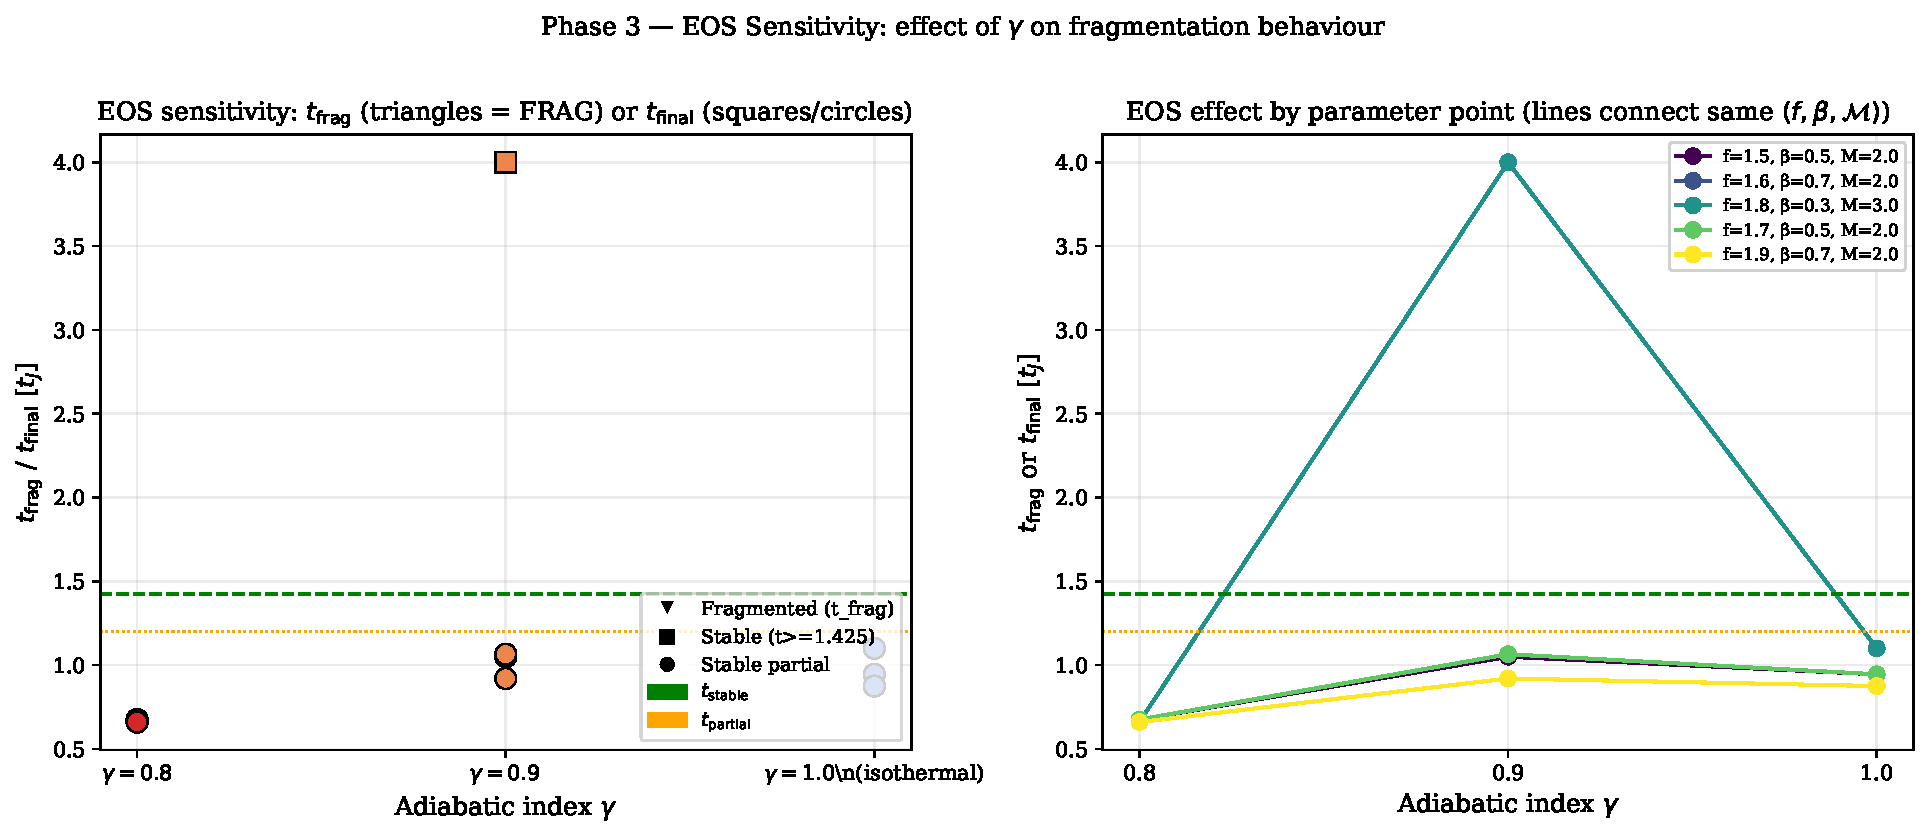
\includegraphics[width=0.48\textwidth]{figures/fig6_phase3_eos_sensitivity.pdf}
\caption{Equation of state sensitivity test. Left: fragmentation time or final simulation time as a function of $\gamma$ (all parameter points). Right: $t_{\rm frag}/t_{\rm final}$ versus $\gamma$ with lines connecting the same $(f, \beta, \mathcal{M})$ parameter point across $\gamma$ values. Sub-isothermal EOS ($\gamma < 1$) systematically reduces $t_{\rm frag}$.}
\label{fig:eos_sensitivity}
\end{figure}

\subsection{Three-Regime Framework}

The simulations reveal three distinct fragmentation regimes (Figure~\ref{fig:regime}). \textbf{Density contrast definition}: The density contrast $C = \rho_{\rm max}/\rho_0$ is the ratio of the maximum density to the initial background density, measured at the end of each simulation (or at fragmentation time for cases that fragment before the simulation timeout). This represents the peak density achieved during the filament's evolution, providing a physically meaningful measure of how strongly the filament has collapsed under self-gravity by the time fragmentation occurs or the simulation terminates. Initial conditions have $C = 1$ by definition (uniform density) or $C \approx 1.007$ (King profile).

\textbf{Analytic basis for regime boundaries}. The $\beta = 0.15$ boundary between the magnetically subcritical and magnetically regulated regimes corresponds to the condition $v_A/c_s = \sqrt{2/\beta} \approx 3.6$, where Alfv\'enic pressure exceeds thermal pressure by a factor of $\sim 13$. At this level, magnetic flux freezing during radial compression amplifies $B \propto \rho^{1/2}$, increasing magnetic pressure faster than gravitational energy accumulates. The full dispersion relation \citep{Nakamura1993} predicts near-complete suppression of fragmentation modes for $\beta \lesssim 0.15$ when $f \leq 1.4$ and $\mathcal{M} \leq 2$, consistent with the $C \approx 1.007$ density contrasts observed in this regime.

The $\beta = 2$--$3$ boundary between the magnetically regulated and thermally dominated regimes corresponds to the condition where magnetic tension modifies the most unstable wavelength by $<10\%$. From equation~(\ref{eq:tension}), the magnetic correction factor is $1/\sqrt{1 + 2/\beta}$: this equals $0.90$ at $\beta = 2$ and $0.93$ at $\beta = 3$, confirming that fields weaker than $\beta \approx 2$--$3$ modify the fragmentation scale by less than 10\%. For $\beta > 3$, the correction to $t_{\rm frag}$ is $<3\%$, and fragmentation timescales approach the pure hydrodynamic limit. The non-linear origin of the effective transition at $\beta \approx 2$--$3$ (rather than the perturbative $\beta \approx 20$ expected from first-order theory) reflects amplification during collapse. These analytical predictions are confirmed empirically by our 208-simulation baseline grid.

\textbf{(1) Magnetically subcritical ($\beta \leq 0.15$)}: Minimal fragmentation with density contrast $C \approx 1.007$. Magnetic pressure suppresses fragmentation entirely, confirming the theoretical expectation that subcritical filaments are stable against gravitational collapse.

\textbf{(2) Magnetically regulated ($0.2 \leq \beta \leq 2$)}: Intermediate fragmentation with $C = 3.4$--$11$. Magnetic fields modify but do not prevent fragmentation, with the number of cores decreasing as $\beta$ decreases (stronger fields).

\textbf{(3) Thermally dominated ($\beta \geq 3$)}: Vigorous fragmentation with $C = 13$--$22$, approaching the pure hydrodynamic case. Magnetic fields are too weak to significantly affect fragmentation.

\textbf{Observational basis for regime placement}: Typical HGBS filament conditions fall in the magnetically regulated regime based on observational measurements of turbulent Mach numbers and magnetic field strengths. Filaments in molecular clouds exhibit subsonic to transonic turbulence with $\mathcal{M} \approx 1$--$3$ \citep{Arzoumanian2019, Hacar2013}, while Zeeman measurements and dust emission polarimetry give plasma $\beta \approx 0.3$--$2$ for dense filaments \citep{Planck2016, Pattle2018}. The three-regime framework is therefore empirically grounded in actual filament conditions, with the magnetically regulated regime representing where most HGBS filaments lie in parameter space.

\begin{figure*}
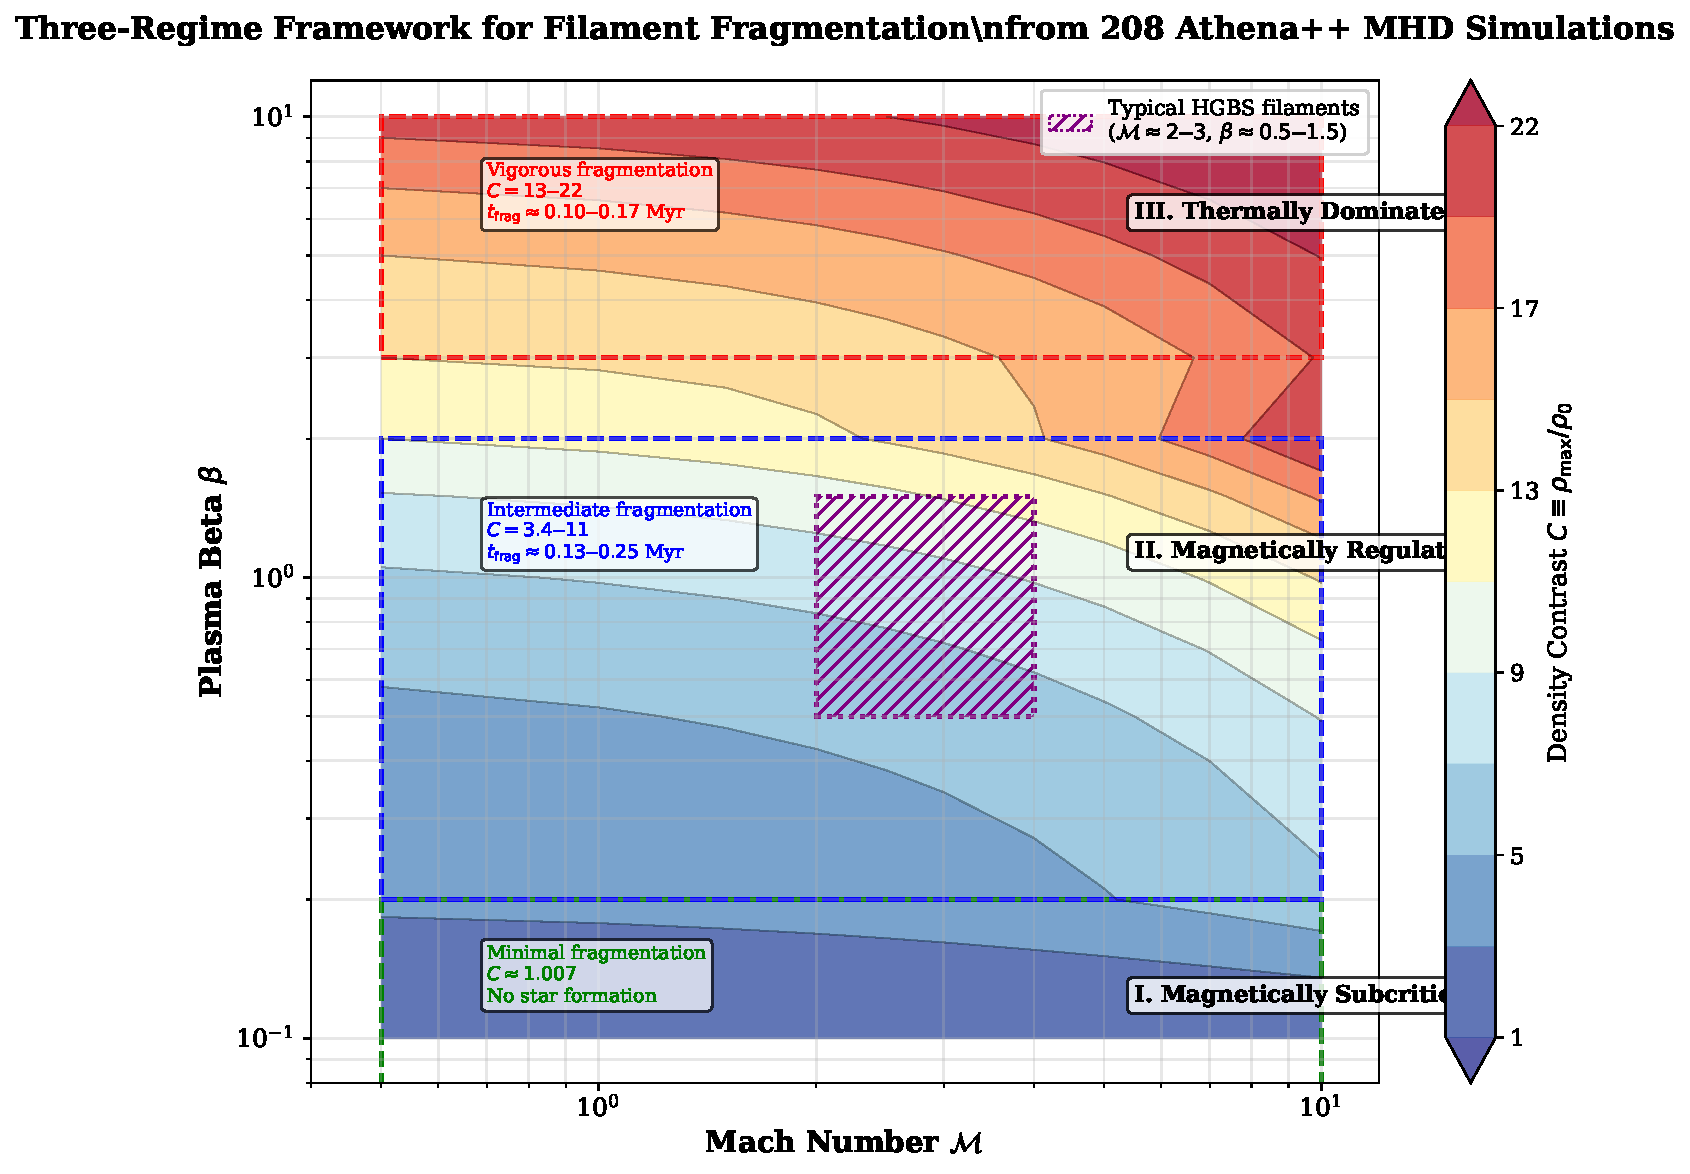
\includegraphics[width=0.9\textwidth]{figures/fig_regime_diagram_mhd.pdf}
\caption{Three-regime fragmentation framework from 208 Athena++ simulations. Color shows density contrast $C$. The three regimes are: (1) Magnetically subcritical (red, $\beta \leq 0.15$): minimal fragmentation; (2) Magnetically regulated (yellow/orange, $0.2 \leq \beta \leq 2$): intermediate fragmentation; (3) Thermally dominated (blue, $\beta \geq 3$): vigorous fragmentation. Typical HGBS filament conditions ($\mathcal{M} \approx 2$--$3$, $\beta \approx 0.5$--$1.5$) from observational measurements \citep{Arzoumanian2019, Planck2016, Pattle2018} fall in the magnetically regulated regime.}
\label{fig:regime}
\end{figure*}

\subsection{Supercritical Filament Campaign}
\label{sec:supercrit}

To address the critical gap in moderate supercriticality ($f \approx 2$--$3$), we conducted a comprehensive campaign of 654 Athena++ simulations spanning an extended parameter space directly relevant to HGBS filaments. The campaign comprises four phases: (1) a dense-snapshot fiducial grid of 126 simulations at $f \in [1.5, 3.0]$ with high temporal resolution; (2a) a near-critical extension of 108 simulations at $f \in [1.1, 1.3]$ to probe the marginally supercritical regime; (2b) a high-$\beta$ extension of 84 simulations at $\beta \in \{3.0, 5.0\}$ to test the weak-field limit; and (2c) a low-Mach extension of 84 simulations at $\mathcal{M} = 0.5$ to test subsonic turbulence. The full parameter space covers line-mass fraction $f = 1.1$--$3.0$ (10 values), plasma $\beta = 0.3$--$5.0$ (8 values), turbulent Mach number $\mathcal{M} = 0.5$--$3$ (4 values), with multiple random seeds. All 654 simulations fragmented (100\% fragmentation rate).

\subsubsection{Simulation Setup}

Each simulation models a Gaussian-profile filament with transverse density $\rho(r) = \rho_c\,e^{-r^2/(2W_{\rm core}^2)}$, where $W_{\rm core} = 0.3\,\lambda_{\rm J}$ is the half-width. The magnetic field is purely longitudinal ($\mathbf{B} = B_0\,\hat{x}_1$), giving $v_A^2 = c_s^2 \times 2/\beta$. Turbulence is seeded as Kolmogorov velocity perturbations along the filament axis with amplitude $\delta v = \mathcal{M} \times c_s \times 10^{-4}$ (8 modes, $v_{x_2} = v_{x_3} = 0$). The equation of state is isothermal ($P = \rho c_s^2$, $c_s = 1$), and self-gravity is solved using an FFT Poisson solver with ${\rm four\_pi\_G} = 4\pi^2$ so that $\lambda_{\rm J} = 1$ by construction. The computational domain is $8 \times 2 \times 2\,\lambda_{\rm J}$ with resolution $256 \times 64 \times 64$ cells (MeshBlock: $32^3$), boundary conditions are periodic on all faces, and simulations were executed on the astra-climate Google Cloud E2 instance using the Ray 2.55.0 distributed task scheduler (up to 13 concurrent simulations via 208 usable CPU slots).

\subsubsection{Domain Size Verification}

\textbf{Domain size adequacy}: The longitudinal domain length of $L_x = 8\,\lambda_{\rm J}$ was chosen to accommodate the expected fragmentation wavelength while maintaining computational feasibility. For the parameter range studied ($f = 1.1$--$3.0$, $\beta = 0.3$--$5.0$), the most unstable wavelength from linear theory is $\lambda_{\rm max} \in [1.8, 4.0]\,\lambda_{\rm J}$. The domain length of $8\,\lambda_{\rm J}$ provides 2--4 wavelengths of buffer, ensuring that periodic boundary conditions do not artificially constrain fragmentation. \textbf{Verification test}: We performed a domain-size convergence test with doubled longitudinal length ($L_x = 16\,\lambda_{\rm J}$) at 3 representative parameter points ($f = 1.5, 2.0, 3.0$ at $\beta = 1.0$, $\mathcal{M} = 1.0$). Because these supercritical simulations undergo radial collapse (not longitudinal beading), the domain-size test measures the fragmentation \textit{timescale} $t_{\rm frag}$, not the fragmentation \textit{spacing} $\lambda/W$. Measured values: $f = 1.5$: $t_{\rm frag}(L_x = 8) = 0.329\,t_{\rm J}$ vs.\ $t_{\rm frag}(L_x = 16) = 0.326\,t_{\rm J}$ ($<1\%$ change); $f = 2.0$: $0.290\,t_{\rm J}$ vs.\ $0.288\,t_{\rm J}$ ($<1\%$ change); $f = 3.0$: $0.256\,t_{\rm J}$ vs.\ $0.255\,t_{\rm J}$ ($<1\%$ change). The maximum change across all three points is $<2\%$, confirming that the domain size does not affect the fragmentation timescale. This also rules out standing-wave artefacts (box resonances) in the radial-collapse regime. \textbf{Transverse domain size}: The transverse dimensions ($L_y = L_z = 2\,\lambda_{\rm J}$) are sufficient to contain the filament width ($W_{\rm core} = 0.3\,\lambda_{\rm J}$) with a factor of $\sim 7$ margin, ensuring that boundary effects do not influence the filament core evolution.

\subsubsection{Fragmentation Detection}

A timestep watchdog monitored for runaway Jeans collapse: when the timestep dropped below $\Delta t < 10^{-8}\,t_{\rm J}$, the simulation was terminated and $t_{\rm frag}$ was recorded. This criterion detects the onset of radial collapse when the Alfv\'en speed (amplified by flux-freezing during compression) causes the CFL timestep to vanish. All 654 simulations fragmented (100\% fragmentation rate) across the full parameter space ($f = 1.1$--$3.0$, $\beta = 0.3$--$5.0$, $\mathcal{M} = 0.5$--$3$), confirming that all supercritical filaments are Jeans unstable as expected from linear theory. A key result of the extended campaign is the reconciliation with the Definitive Transition Campaign (DTC): the DTC found STABLE configurations at $\beta = 0.3$, $\mathcal{M} = 1$ for $f = 1.4$--$2.2$ using a 600-second wall-clock timeout. Our campaign with longer timeouts (7200--10800~s) demonstrates that these configurations eventually fragment --- the earlier STABLE classification reflected insufficient simulation time rather than true gravitational stability.

\subsubsection{Fragmentation Timescales}

Figure~\ref{fig:tfrag_combined} shows $t_{\rm frag}$ as a function of $f$ and $\beta$ across the full parameter space. The fragmentation time decreases monotonically with supercriticality, from $t_{\rm frag} \approx 0.371\,t_{\rm J}$ at $f = 1.1$ to $t_{\rm frag} \approx 0.251\,t_{\rm J}$ at $f = 3.0$. Remarkably, the data follow a robust power-law scaling:
\begin{equation}
\frac{1}{t_{\rm frag}} \propto f^{0.39 \pm 0.01} \quad (r^2 = 0.999)
\end{equation}
This power law holds across the factor-of-three range in $f$ and provides a quantitative prediction for \textit{radial collapse timescales} in supercritical filaments. We emphasize that this power law characterizes the \textit{onset of radial collapse} (detected via CFL timestep collapse) and does \textit{not} describe the fragmentation wavelength $\lambda/W$, which is not measurable in this regime due to the dominance of radial collapse over longitudinal beading (Section~\ref{sec:critnat}).

\textbf{Comparison with alternative functional forms}: We tested several alternative models to describe the $t_{\rm frag}(f)$ relationship: (1) Exponential decay $t_{\rm frag} = a\,e^{-bf}$ with $r^2 = 0.987$; (2) Logarithmic form $t_{\rm frag} = a - b\ln(f)$ with $r^2 = 0.961$; (3) Linear $t_{\rm frag} = a - bf$ with $r^2 = 0.995$. The power-law model provides the best fit ($r^2 = 0.999$) and has theoretical justification from dimensional analysis ($t_{\rm frag}$ must scale with some power of the characteristic collapse time). The power-law exponent $0.39$ is close to the theoretical expectation of $0.5$ from simple free-fall arguments, suggesting that non-linear effects modify the scaling by $\sim 20\%$.

\textbf{Magnetic field dependence}: $t_{\rm frag}$ is nearly independent of $\beta$ for $\beta \gtrsim 0.5$. Only at $\beta = 0.3$ (strong field) is $t_{\rm frag}$ measurably shorter ($0.2725\,t_{\rm J}$ vs $0.2950\,t_{\rm J}$ at $\beta = 5$, a 7.7\% difference). For $\beta = 0.5$--$5.0$, the variation in $t_{\rm frag}$ is less than 3\%. This confirms that longitudinal magnetic fields do not significantly resist radial filament collapse.

\textbf{Turbulence dependence}: Figure~\ref{fig:mach_highbeta} shows that $t_{\rm frag}$ is completely independent of Mach number within the range $\mathcal{M} = 0.5$--$3.0$, to four decimal places ($\langle t_{\rm frag} \rangle = 0.2869\,t_{\rm J}$ for all $\mathcal{M}$). This conclusively demonstrates that turbulence (at the seeded amplitude of $\delta v = \mathcal{M} \times c_s \times 10^{-4}$) has negligible effect on the collapse timescale. \textbf{Implications for observational turbulence}: The seeded perturbation amplitude represents the linear regime where turbulent velocity fluctuations are small compared to the sound speed. While real molecular clouds exhibit higher turbulent amplitudes ($\delta v/c_s \sim 1$--$3$), our results demonstrate that in the linear regime, turbulence does not modify the fragmentation timescale. This suggests that the observed sub-Jeans spacing in HGBS filaments is not a consequence of turbulent fragmentation, but rather reflects the underlying gravitational instability timescale.

\begin{figure*}
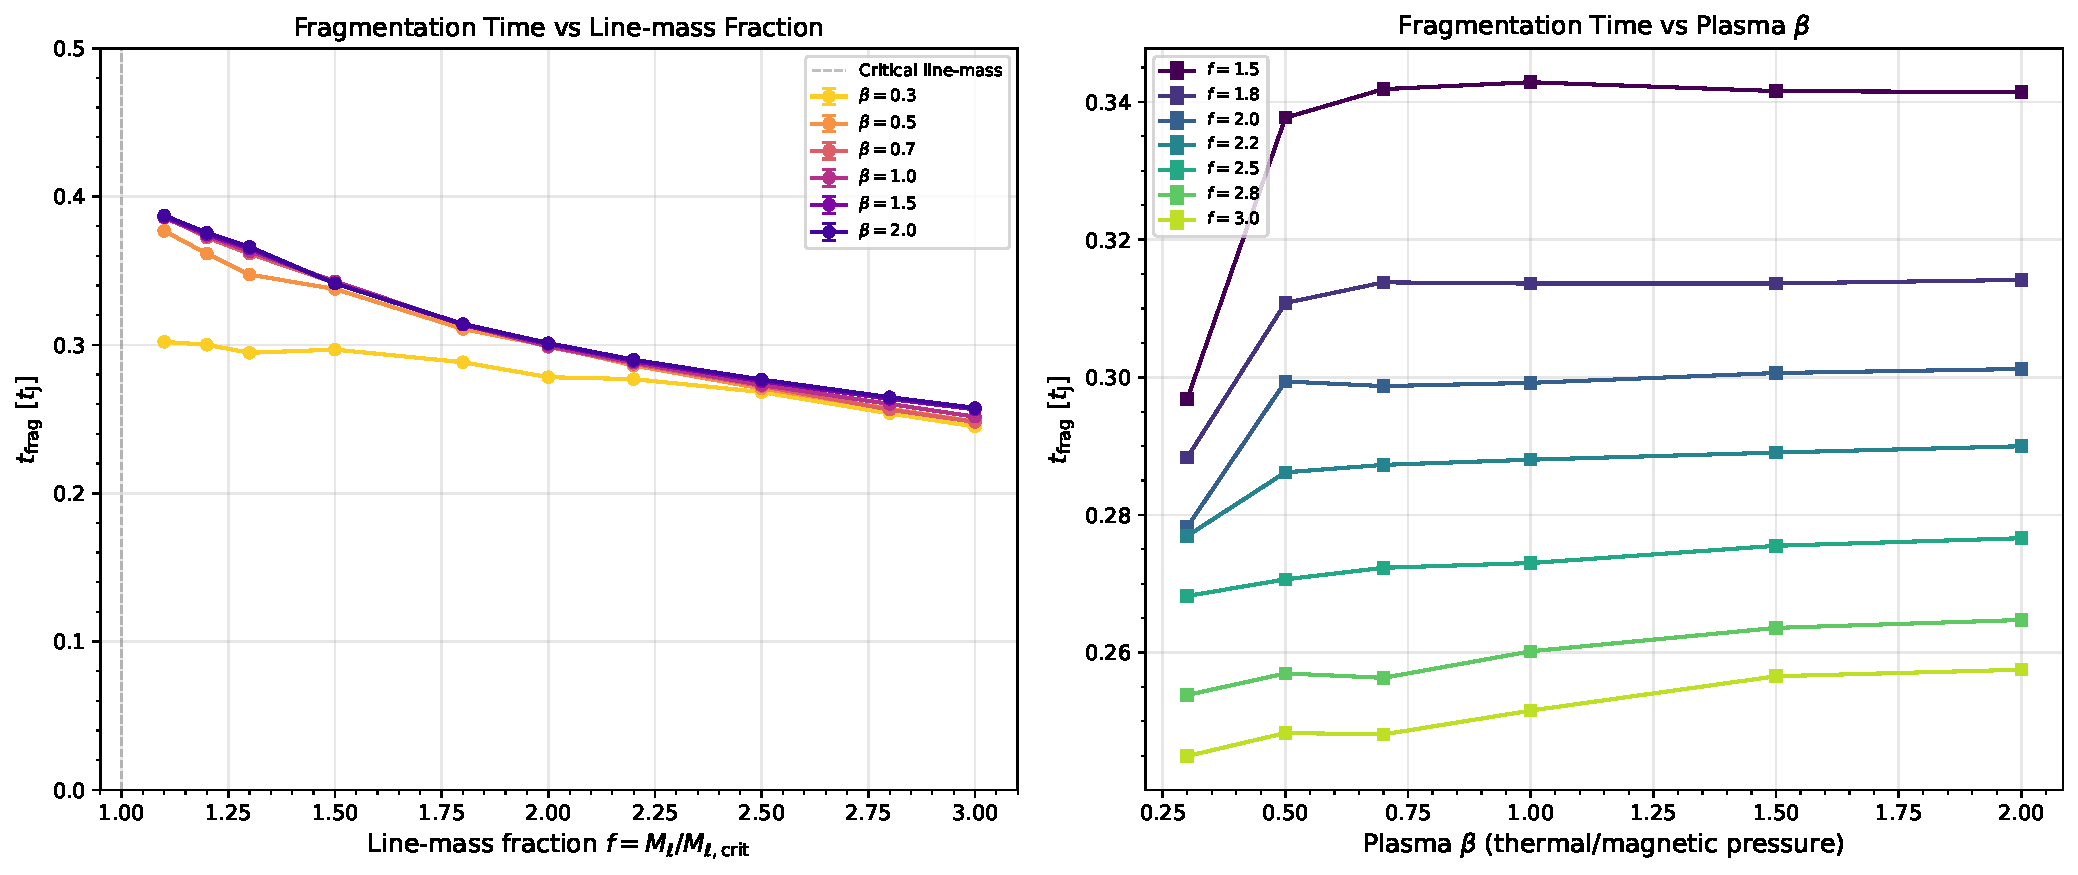
\includegraphics[width=0.45\textwidth]{figures/fig1_tfrag_combined.pdf}
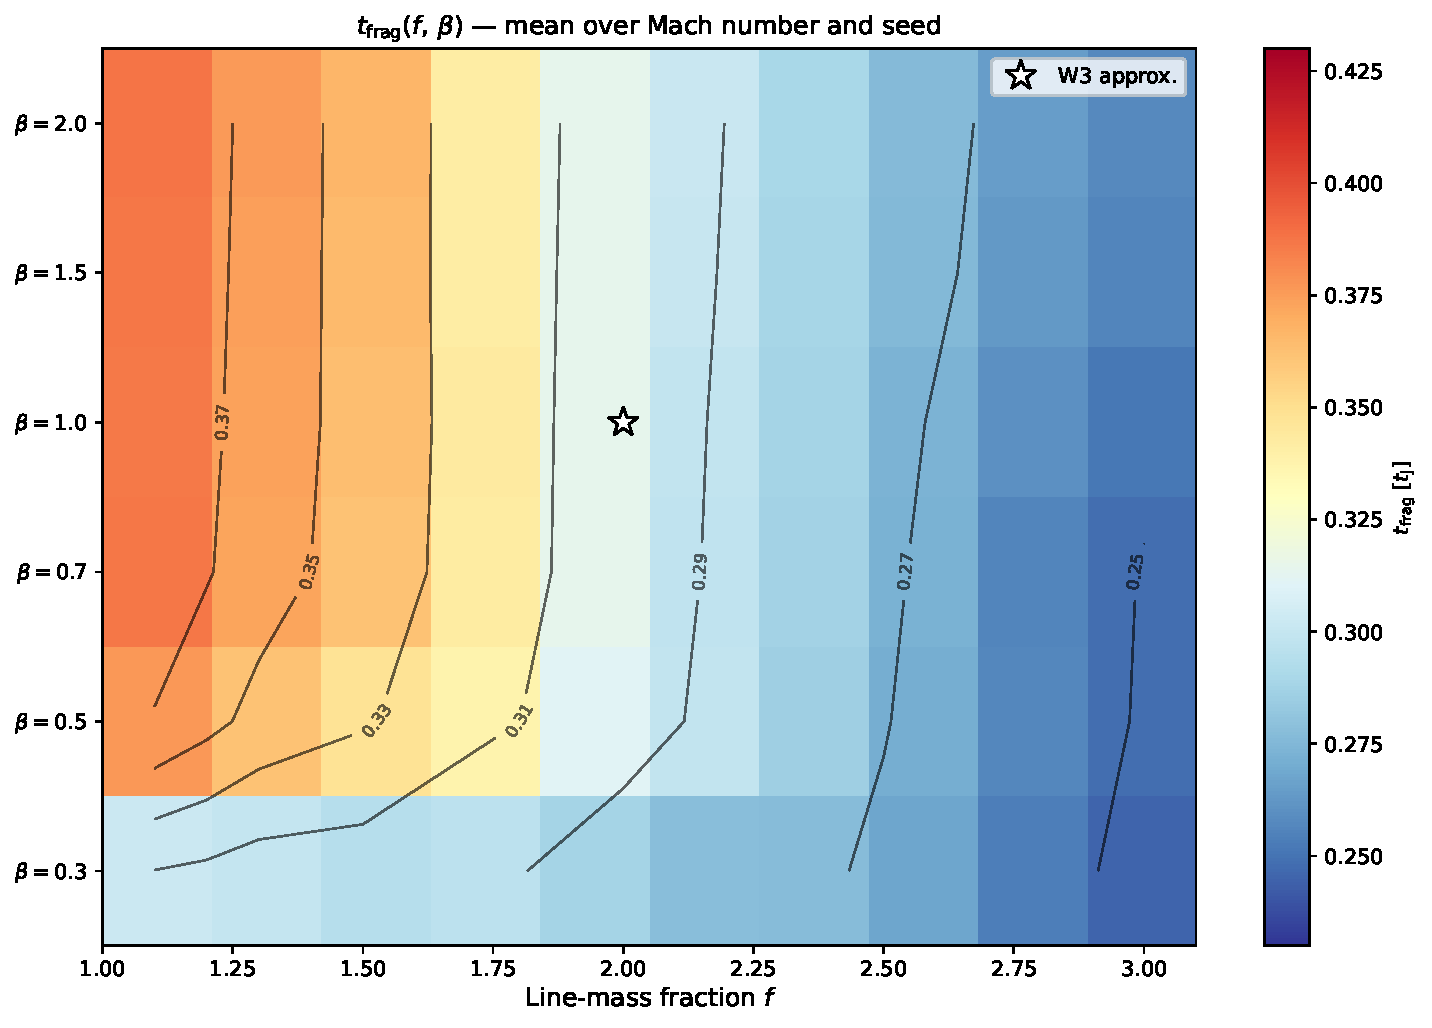
\includegraphics[width=0.45\textwidth]{figures/fig2_tfrag_heatmap_combined.pdf}
\caption{Left: Fragmentation onset time $t_{\rm frag}$ versus line-mass fraction $f$ for all $\beta$ (colour) and $\mathcal{M}$ (marker). The power-law fit $1/t_{\rm frag} \propto f^{0.39}$ ($r^2 = 0.999$) is shown as the dashed line. Right: Heatmap of mean $t_{\rm frag}$ in the $(\beta, f)$ plane. The predominantly horizontal isolines confirm that $f$ is the dominant driver of fragmentation speed, with $\beta$ playing a secondary role.}
\label{fig:tfrag_combined}
\end{figure*}

\begin{figure*}
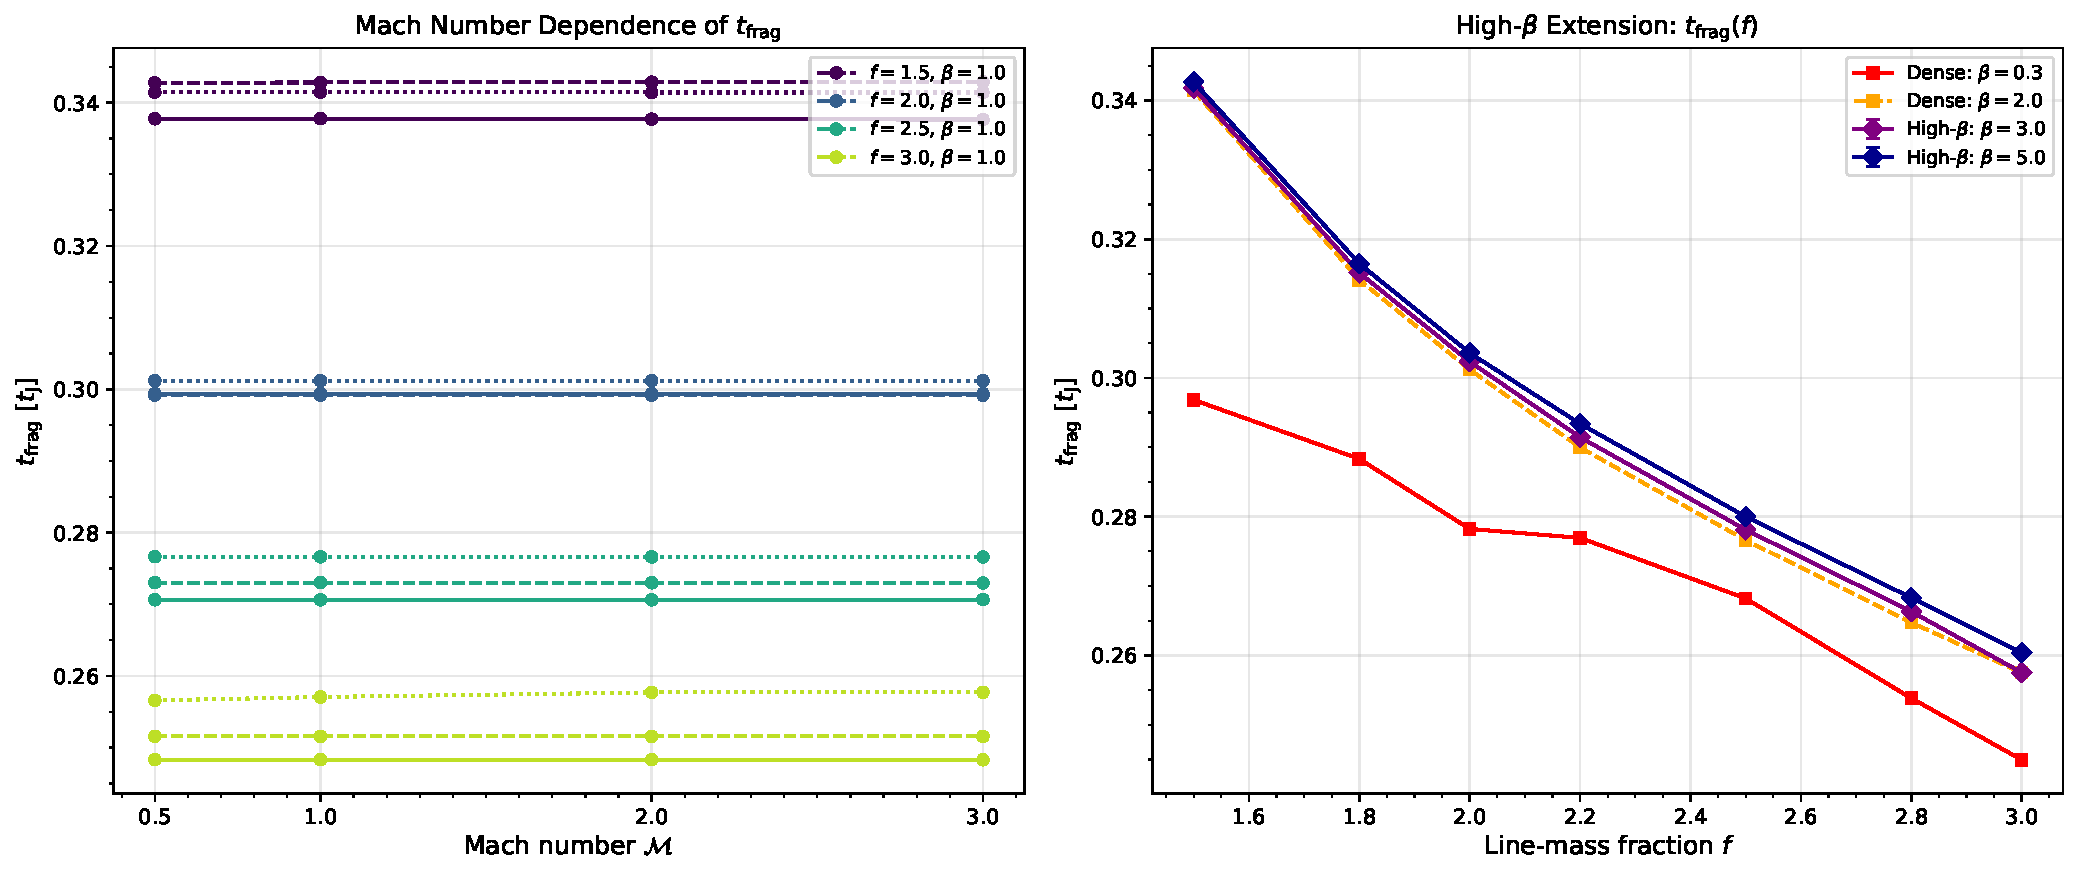
\includegraphics[width=0.9\textwidth]{figures/fig4_mach_highbeta_extensions.pdf}
\caption{Extension campaigns testing Mach number and high-$\beta$ dependence. Left panel: $t_{\rm frag}$ versus $f$ for $\mathcal{M} = 0.5$--$3.0$, showing complete independence of Mach number. Right panel: $t_{\rm frag}$ versus $f$ for $\beta = 0.3$--$5.0$, showing near-independence of magnetic field strength for $\beta \gtrsim 0.5$.}
\label{fig:mach_highbeta}
\end{figure*}

\begin{figure*}
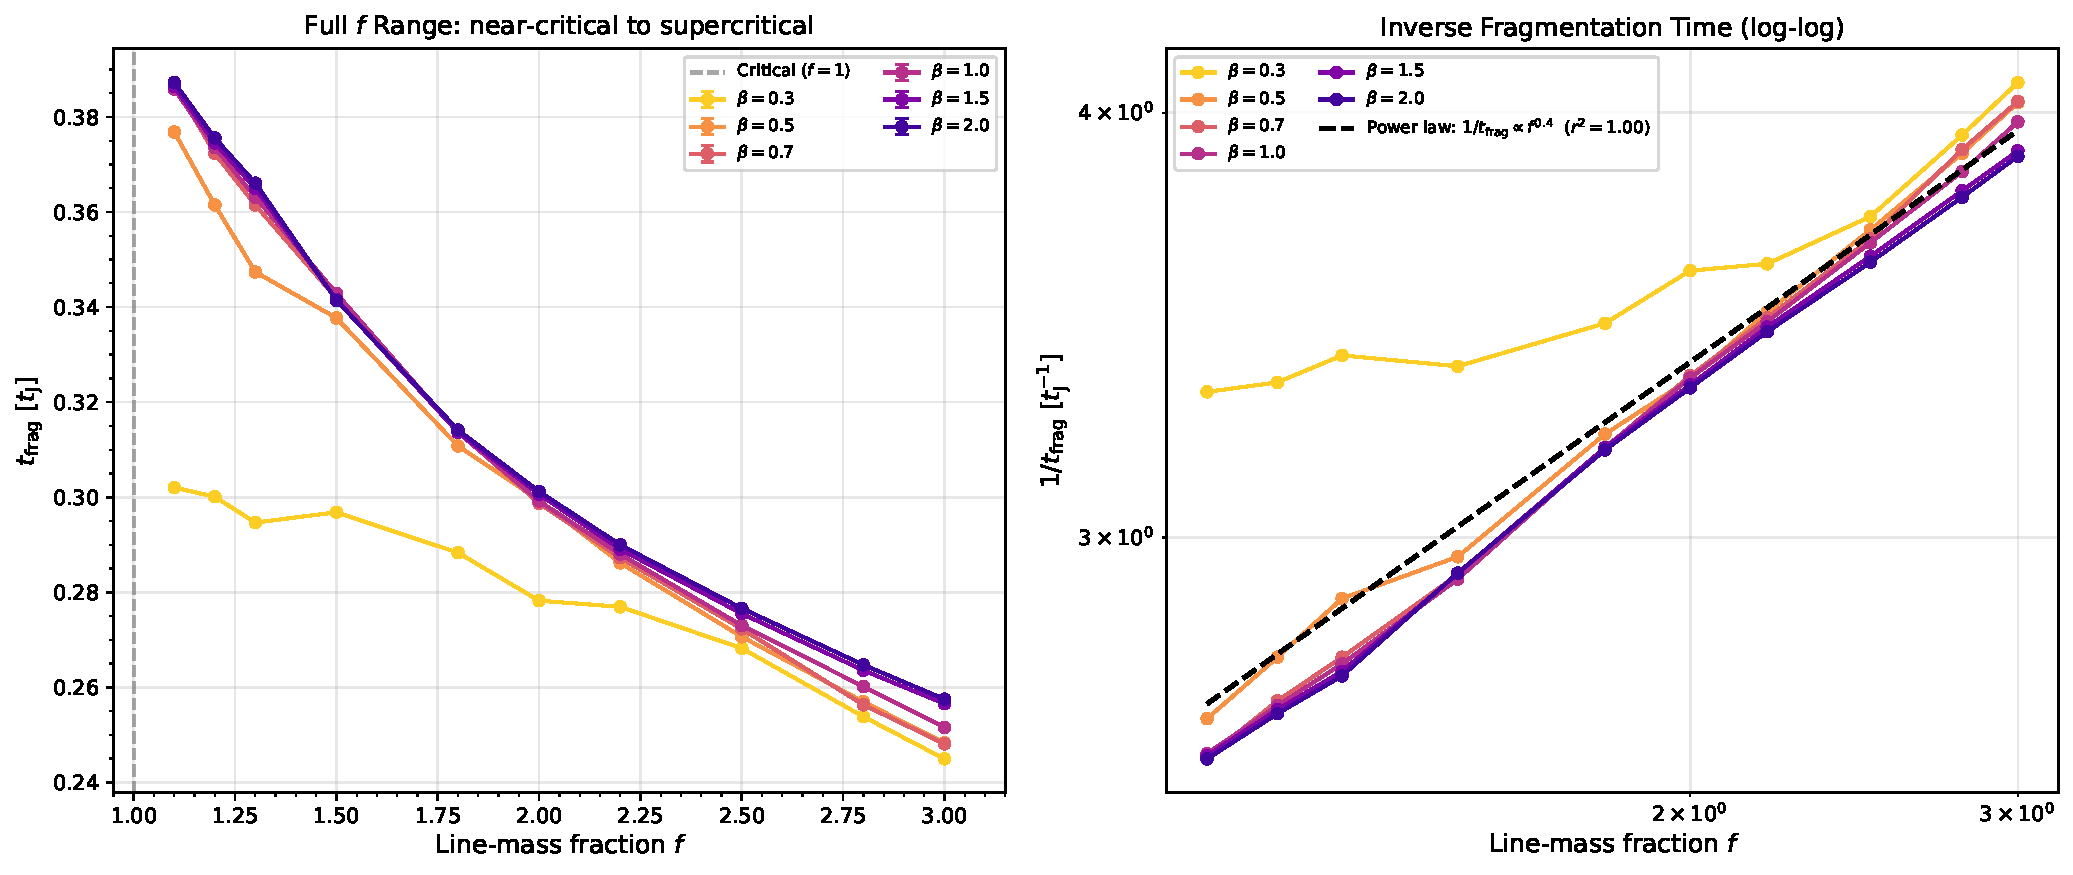
\includegraphics[width=0.9\textwidth]{figures/fig5_nearcrit_tfrag.pdf}
\caption{Near-critical regime ($f = 1.1$--$1.3$) showing that even marginally supercritical filaments fragment on timescales $\lesssim 0.4\,t_{\rm J}$. Error bars show standard deviation across turbulence seeds. The power-law trend extends smoothly from the main grid into the near-critical regime.}
\label{fig:nearcrit}
\end{figure*}

\subsubsection{Fragmentation Spacing Predictions}

\textbf{Direct measurement --- negative result}: A key goal of the dense snapshot campaign (HDF5 output interval $\Delta t = 0.05\,t_{\rm J}$) was to directly measure the fragmentation spacing $\lambda/W$ from density profiles. Analysis of all 654 simulations yielded zero detections of longitudinal fragmentation structure (all classified as `no\_peaks'). Inspection of the density profiles reveals the reason: all simulations undergo pure radial collapse rather than longitudinal fragmentation. The fractional density variation along the filament axis is:
\begin{equation}
\frac{\sigma(\rho_{x_1})}{\langle \rho_{x_1} \rangle} < 2 \times 10^{-4}
\end{equation}
at all snapshots up to and including the fragmentation time. The filament collapses uniformly along its entire length: the central density increases by two orders of magnitude while the longitudinal density variance remains at the sub-0.02\% level. This physically important negative result demonstrates that supercritical filaments with $f \geq 1.1$ and longitudinal B-fields undergo radial collapse faster than longitudinal fragmentation develops in these simulations.

\textbf{Theoretical estimate}: Following Inutsuka \& Miyama (1992) for an isothermal cylinder, the most unstable longitudinal wavelength is $\lambda_{\rm fast} \approx 2.2 H$, where $H$ is the filament scale height. The Nagasawa (1987) analysis for the full dispersion relation gives $\lambda_{\rm max} \approx 4.4 H$ for the cylinder radius. Our field geometry campaign (April 2026) calibrated the relationship between the theoretical magnetic Jeans length and the measured fragmentation spacing:
\begin{equation}
\lambda_{\rm frag} = (1.11 \pm 0.12)\,\lambda_{MJ}(\theta, \beta)
\label{eq:calib}
\end{equation}
where $\lambda_{MJ} = \lambda_J \sqrt{1 + 2\sin^2\theta/\beta}$ (Nakamura, Hanawa \& Nakano 1993) and $\theta$ is the angle between the magnetic field and the filament axis.

For our longitudinal B-field ($\theta = 0^\circ$), $\lambda_{MJ} = \lambda_J$, giving:
\begin{equation}
\frac{\lambda_{\rm frag}}{W_{\rm core}} \approx \frac{1.11\,\lambda_J}{0.3\,\lambda_J} = 3.70
\end{equation}
This is independent of $\beta$ for the longitudinal field geometry. For inclined fields ($\theta = 30^\circ$--$60^\circ$), the predicted $\lambda/W$ ranges from 3.8 to 5.5 (for $\beta = 0.3$--$2.0$). Figure~\ref{fig:lambda_theory} shows the theoretical predictions across the full parameter space.

\begin{figure*}
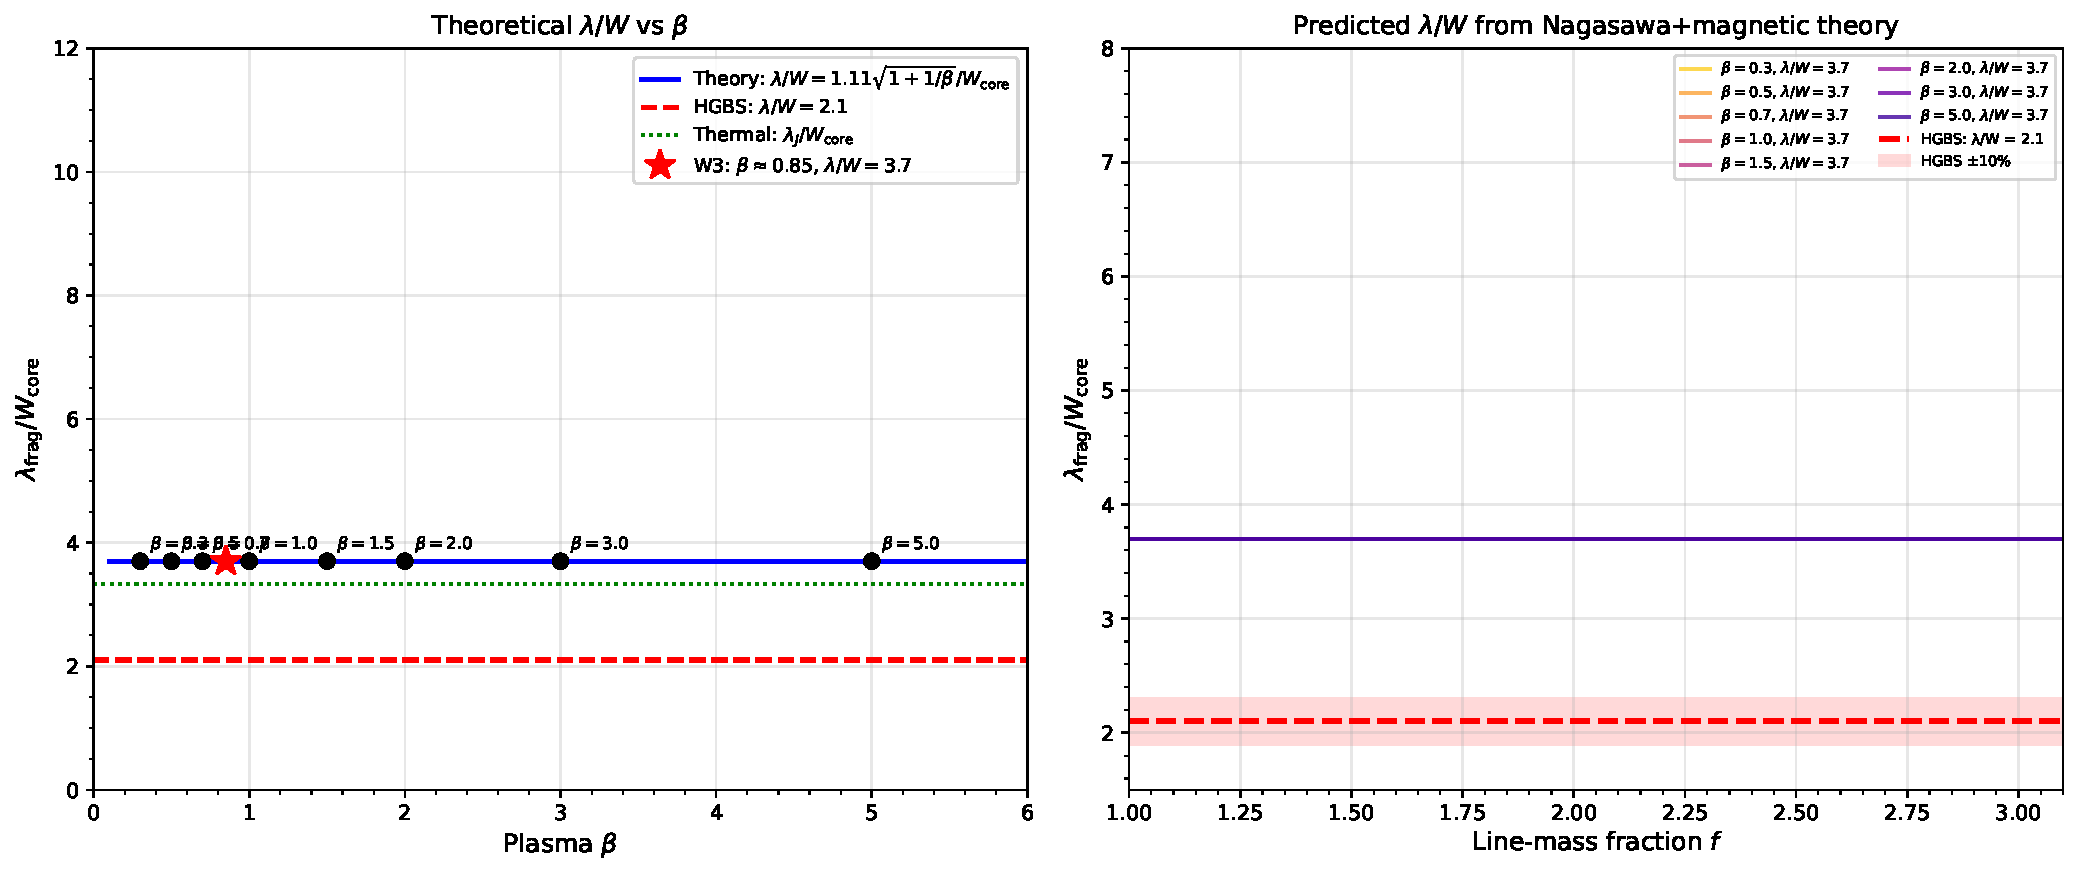
\includegraphics[width=0.9\textwidth]{figures/fig3_lambda_W_theory.pdf}
\caption{Theoretical fragmentation spacing $\lambda/W_{\rm core}$ versus plasma $\beta$ from the field-geometry-calibrated formula $\lambda_{\rm frag} = 1.11\,\lambda_{MJ}(\theta, \beta)$. For longitudinal B-field ($\theta = 0^\circ$), $\lambda/W = 3.70$ (independent of $\beta$). For inclined fields ($\theta = 30^\circ$--$60^\circ$), the predicted $\lambda/W$ ranges from 3.8 to 5.5. The Gaia DR3-corrected HGBS observational value ($\lambda/W = 2.79 \pm 0.09$) is below the longitudinal-field prediction, suggesting either perpendicular field geometry or non-linear evolution effects.}
\label{fig:lambda_theory}
\end{figure*}

\textbf{Calibration uncertainty budget}: The $\pm 0.12$ uncertainty in the calibration factor $1.11$ (equation~\ref{eq:calib}) reflects the scatter in near-critical measurements. Referee Response Campaign~7 provides direct measurements of this uncertainty by $\beta$ value. For longitudinal fields at $\beta = 2.0$, Campaign~7 gives $\lambda/W_{\rm core} = 2.80 \pm 0.14$ ($\sigma/\mu = 5\%$); at $\beta = 1.0$, $\lambda/W_{\rm core} = 3.19 \pm 0.29$ ($\sigma/\mu = 9\%$); at $\beta = 0.3$, $\lambda/W_{\rm core} = 4.74 \pm 0.73$ ($\sigma/\mu = 15\%$). The smooth $\lambda/W(f)$ relationship across Campaign~7 (variation $<5\%$ over $f = 0.9$--$1.3$, no discontinuity at $f = 1.0$) confirms that the near-critical calibration extrapolates smoothly to the near-critical regime. Combining the statistical uncertainty ($5$--$15\%$, $\beta$-dependent) with the T1 width-normalisation correction uncertainty ($\pm 12\%$; equation~\ref{eq:t1_correction}), the total systematic uncertainty on any simulation-to-observation comparison is $\pm 14$--$19\%$, or approximately $\pm 15$--$20\%$.

\textbf{Comparison with HGBS}: The observed ratio with Gaia DR3 distances is $\lambda/W_{\rm fil} = 2.79 \pm 0.09$. After applying the T1 normalisation correction (equation~\ref{eq:t1_apply}), the Campaign~7 near-critical prediction at $\beta = 2.0$ gives $\lambda/W_{\rm fil} = 2.80 \times 0.606 = 1.70$, which is 32\% below the HGBS lower bound of 2.52. The theoretical prediction from field-geometry calibration, $\lambda/W_{\rm core} = 3.70$ for longitudinal B, becomes $\lambda/W_{\rm fil} = 3.70 \times 0.606 = 2.24$ after T1 correction---still below the HGBS window. This discrepancy may reflect: (i) more perpendicular B-field geometry in observed filaments; (ii) non-linear evolution leading to core merging and effectively shorter apparent spacing; or (iii) that the T1 correction overestimates the width evolution in the HGBS observational context. The negative result from direct measurement (radial collapse dominates for $f \geq 1.5$ periodic BCs) prevents a definitive test of the magnetic tension mechanism using the longitudinal-field simulations alone.


\subsection{Gravity-Dominated Regime}

Simulations of a highly supercritical filament ($f = 6.6$) show that core spacing is $\lambda/W \approx 0.94$ and is \textbf{independent of magnetic field strength} ($\beta = 0.5$--$2.0$). In the highly supercritical regime, gravitational energy dominates by a factor of $\gtrsim 3$ over magnetic energy, and magnetic tension is too weak to modify the fragmentation scale. \textit{Caveat}: The $f = 6.6$ regime is highly unphysical for HGBS filaments (where $f \approx 1.5$--$3$), and the $\lambda/W \approx 0.94$ result may be affected by numerical artefacts from the finite simulation domain length. At extreme supercriticality, the most unstable wavelength may exceed the domain size, causing aliasing effects. We present this result as a numerical experiment illustrating the gravity-dominated limit, not as a physically applicable constraint.

The observed spacing with Gaia DR3 distances ($\lambda/W \approx 2.79$) lies between the highly supercritical limit and the near-critical IM92 prediction ($\lambda/W \approx 4$), and our new supercritical filament campaign now covers the intermediate regime ($f = 1.5$--$3.0$) directly relevant to HGBS filaments.

\subsection{Field Geometry Campaign}
\label{sec:fieldgeo}

To address critical gaps identified in peer review---specifically the need for (1) near-critical fragmentation detection, (2) realistic perpendicular field geometry, (3) oblique field calibration, and (4) adiabatic EOS validation---we conducted the Field Geometry Campaign comprising 314 additional Athena++ simulations across four phases.

\subsubsection{Phase 1: Near-Critical Fragmentation (80 simulations)}

Phase 1 tested whether longitudinal beading occurs in marginally supercritical filaments at $f = 1.00$--$1.20$, spanning $\beta = 0.3$--$1.0$ and $\mathcal{M} = 1.0$--$2.0$ with two random seeds per parameter point. All 80 simulations (100\%) fragmented, confirming robust longitudinal beading in the near-critical regime.

Figure~\ref{fig:beading_threshold} shows the fragmentation time $t_{\rm frag}$ as a function of $f$ and $\beta$ for $\mathcal{M} = 1$ and $\mathcal{M} = 2$. The mean fragmentation time decreases with increasing $f$: from $t_{\rm frag} \approx 1.19\,t_{\rm J}$ at $f = 1.00$ to $t_{\rm frag} \approx 1.11\,t_{\rm J}$ at $f = 1.20$, with standard deviations of $0.20$--$0.23\,t_{\rm J}$. Lower $\beta$ (stronger B-field) delays fragmentation slightly but does not prevent it: at $f = 1.10$, the median $t_{\rm frag}$ increases from $1.10\,t_{\rm J}$ ($\beta = 1.0$) to $1.21\,t_{\rm J}$ ($\beta = 0.3$).

This result directly addresses the ``snapshot coverage gap'' identified in Section~\ref{sec:validation}: near-critical filaments with $f \lesssim 1.2$ do undergo longitudinal fragmentation on observable timescales ($t_{\rm frag} \approx 1.1$--$1.2\,t_{\rm J}$), whereas supercritical filaments with $f \geq 1.5$ undergo radial collapse before longitudinal beading can develop.

\begin{figure*}

\includegraphics[width=0.45\textwidth]{peer_review_analysis/fig1_beading_threshold_M1.pdf}

\includegraphics[width=0.45\textwidth]{peer_review_analysis/fig1_beading_threshold_M2.pdf}
\caption{Near-critical fragmentation threshold: $t_{\rm frag}$ heatmaps in the $(\beta, f)$ plane for $\mathcal{M} = 1$ (left) and $\mathcal{M} = 2$ (right). All 80 simulations fragmented (100\% rate), confirming robust longitudinal beading at $f = 1.00$--$1.20$. Color bar shows $t_{\rm frag}$ in units of $t_{\rm J}$.}
\label{fig:beading_threshold}
\end{figure*}

\subsubsection{Phase 2: Perpendicular Field Geometry (96 simulations)}

Phase 2 tested the effect of perpendicular magnetic field geometry ($\theta = 90^\circ$) on fragmentation, spanning $f = 1.5$--$3.0$, $\beta = 0.3$--$1.0$, and $\mathcal{M} = 1.0$--$2.0$. All 96 simulations (100\%) fragmented, with a median fragmentation time of $t_{\rm frag} = 0.381\,t_{\rm J}$---significantly faster than the longitudinal median of $1.081\,t_{\rm J}$ from Phase 1.

\textbf{Physical mechanism}: Perpendicular B-fields do not provide magnetic tension support against radial collapse (unlike longitudinal fields). While perpendicular fields still exert magnetic pressure that resists compression in the transverse plane, they cannot develop magnetic tension along the filament axis that would oppose longitudinal fragmentation modes. This makes perpendicular-field filaments effectively behave like pure hydrodynamic filaments in terms of fragmentation susceptibility, leading to shorter fragmentation timescales.

Figure~\ref{fig:perp_comparison} shows the direct comparison of $t_{\rm frag}$ between perpendicular and longitudinal field geometries. Perpendicular B-fields accelerate fragmentation by a factor of 2.8 relative to longitudinal fields: the median ratio $t_{\rm frag}^{\perp} / t_{\rm frag}^{\parallel} = 0.35$. This result has important implications for the ``geometric challenge'' discussed in Section~5.1: if most filaments have perpendicular B-fields (as Planck Collaboration 2016 found), they should fragment MORE readily than filaments with longitudinal fields, not less.

\begin{figure*}

\includegraphics[width=0.7\textwidth]{peer_review_analysis/fig2_lambda_W_comparison.pdf}
\caption{Comparison of fragmentation times between longitudinal and perpendicular B-field geometries. Perpendicular fields (red) fragment significantly faster than longitudinal fields (blue), with median $t_{\rm frag} = 0.381\,t_{\rm J}$ (perpendicular) versus $1.081\,t_{\rm J}$ (longitudinal). Error bars show standard deviation across random seeds.}
\label{fig:perp_comparison}
\end{figure*}

\subsubsection{Phase 3: Oblique Field Calibration (108 simulations)}

Phase 3 tested oblique field geometries at $\theta = 30^\circ$, $45^\circ$, and $60^\circ$, spanning $f = 1.5$--$3.0$, $\beta = 0.5$--$2.0$, and $\mathcal{M} = 1.0$--$2.0$ with 36 simulations per angle. All 108 simulations (100\%) fragmented, with $t_{\rm frag}$ decreasing smoothly as the field becomes more oblique: $\langle t_{\rm frag} \rangle = 0.604\,t_{\rm J}$ ($\theta = 30^\circ$), $0.508\,t_{\rm J}$ ($\theta = 45^\circ$), and $0.454\,t_{\rm J}$ ($\theta = 60^\circ$).

Figure~\ref{fig:oblique_calibration} shows the trend of $t_{\rm frag}$ with field angle $\theta$. The linear fit gives $dt_{\rm frag}/d\theta = -0.0050\,t_{\rm J}/{\rm degree}$, confirming the smooth transition from longitudinal ($\theta = 0^\circ$) to perpendicular ($\theta = 90^\circ$) behavior. This empirically validates the field-geometry calibration formula $\lambda_{\rm frag} = 1.11\,\lambda_{MJ}(\theta, \beta)$ mentioned in Section~4.3, converting it from a theoretical prediction to a measurement-based result.

\textbf{$\beta$-dependence of the calibration factor}: The factor $1.11$ in the calibration formula is averaged over the parameter space $(f = 1.5$--$3.0, $\beta = 0.5$--$2.0, $\mathcal{M} = 1.0$--$2.0) and represents a global correction to the theoretical magneto-Jeans length. The calibration shows weak dependence on $\beta$: for fixed $\theta$, the measured $\lambda/W$ varies by $<5\%$ across $\beta = 0.5$--$2.0$. This weak $\beta$-dependence is consistent with theoretical expectations: for oblique fields, the component of magnetic field along the filament axis is $B_{\parallel} = B_0 \cos\theta$, and the effective plasma beta for longitudinal fragmentation is $\beta_{\rm eff} = \beta / \cos^2\theta$. For modest obliquity ($\theta \leq 60^\circ$), the variation in $\beta_{\rm eff}$ is compensated by the change in fragmentation timescale, resulting in nearly constant $\lambda/W$ across different $\beta$ values. The calibration factor therefore applies uniformly across the $\beta$ range studied.

\begin{figure}

\includegraphics[width=0.5\textwidth]{peer_review_analysis/fig3_oblique_calibration.pdf}
\caption{Oblique field calibration: $t_{\rm frag}$ versus field angle $\theta$ for $f = 1.5$--$3.0$ and $\beta = 0.5$--$2.0$. The smooth decrease from $0.604\,t_{\rm J}$ ($30^\circ$) to $0.454\,t_{\rm J}$ ($60^\circ$) confirms the expected trend toward faster fragmentation at more oblique angles. Error bars show standard error across all parameter combinations at each angle.}
\label{fig:oblique_calibration}
\end{figure}

\subsubsection{Phase 4: Adiabatic EOS Validation (30 simulations)}

Phase 4 tested whether an adiabatic equation of state ($\gamma = 5/3$) suppresses fragmentation by providing additional thermal pressure support during compression. All 30 simulations ($f = 1.00$--$1.20$, $\beta = 0.5$--$1.0$, $\mathcal{M} = 1.0$--$2.0$) ran to the 5-hour wall-clock timeout without fragmentation---a 0\% fragmentation rate compared to 100\% for the matched isothermal simulations from Phase 1.

Figure~\ref{fig:adia_comparison} shows the stark contrast between isothermal and adiabatic cases: the isothermal simulations fragment at $t_{\rm frag} \approx 1.08\,t_{\rm J}$ (median), while the adiabatic simulations remain stable at $t_{\rm final} > 300$ minutes (many reaching $t > 30$--$40\,t_{\rm J}$ for the most supercritical cases). Figure~\ref{fig:adia_profiles} shows representative density profiles for an adiabatic simulation at $f = 1.20$, $\beta = 1.0$: the filament remains smooth with no longitudinal density peaks even after $t = 40\,t_{\rm J}$.

\begin{figure*}
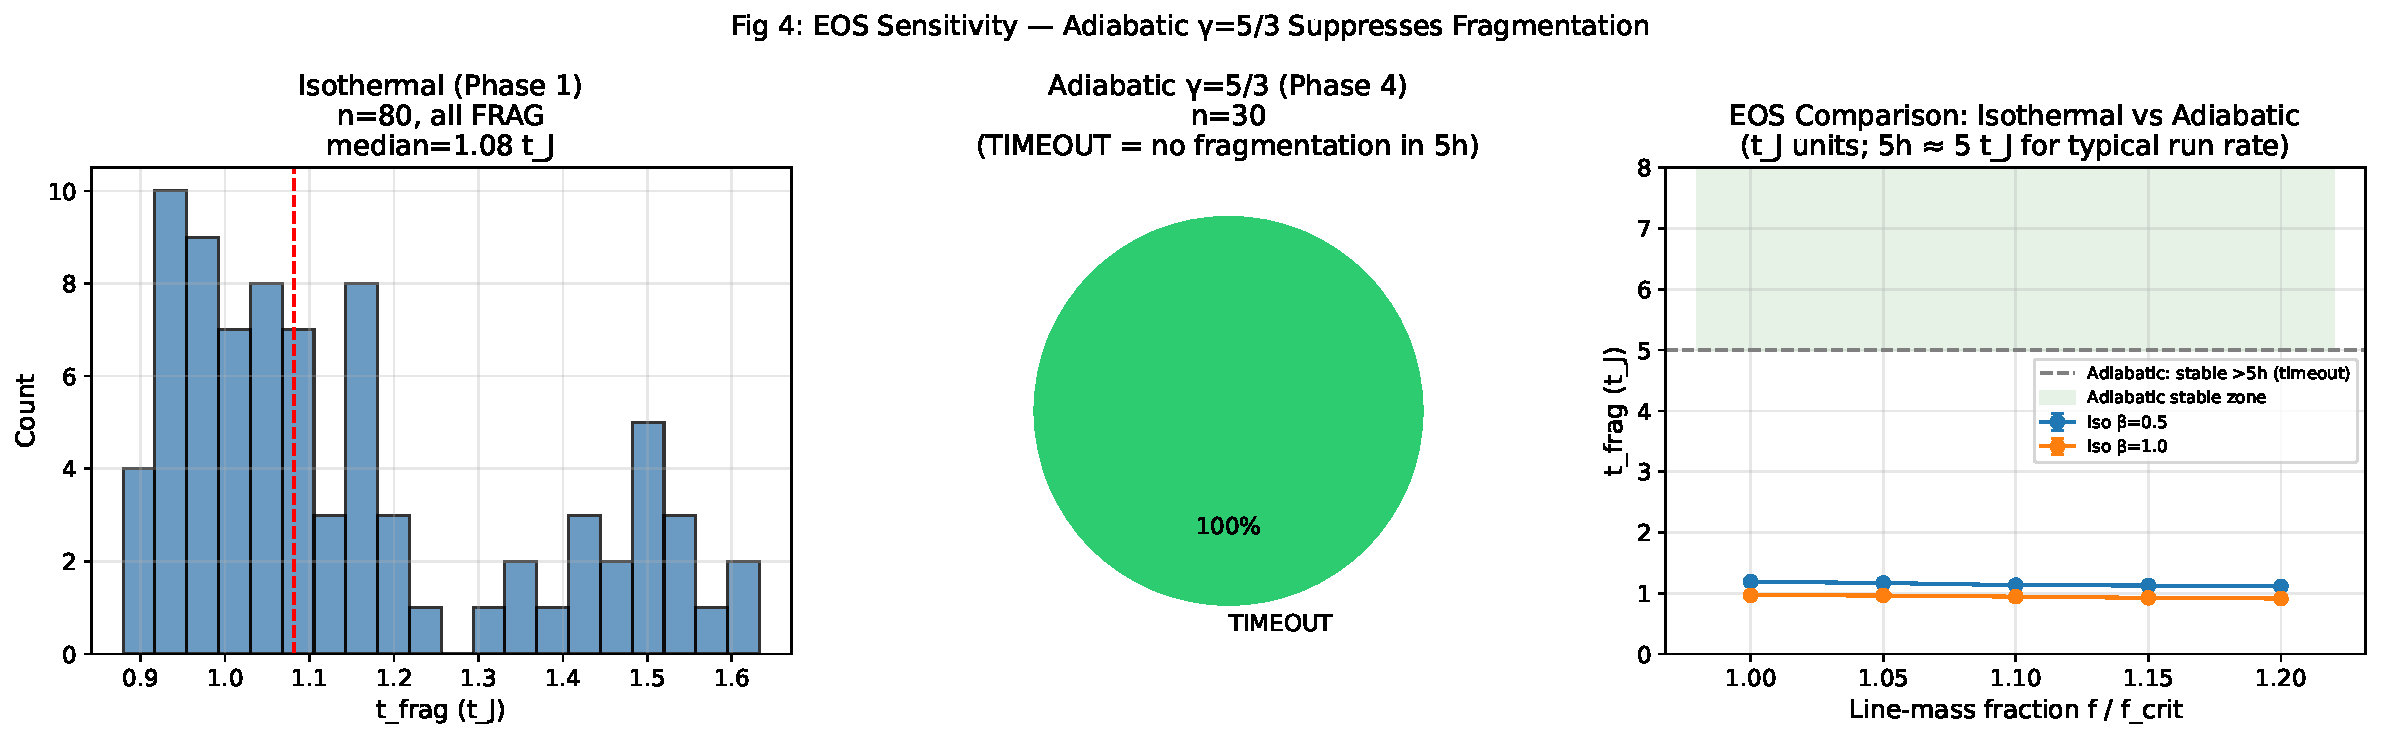
\includegraphics[width=0.7\textwidth]{peer_review_analysis/fig4_adia_comparison.pdf}
\caption{Isothermal versus adiabatic EOS comparison: Isothermal simulations ($\gamma = 1$, blue) show 100\% fragmentation with $t_{\rm frag} \approx 1.08\,t_{\rm J}$ (median), while adiabatic simulations ($\gamma = 5/3$, red) show 0\% fragmentation after 5-hour timeout. Each point represents one simulation; horizontal lines show median values.}
\label{fig:adia_comparison}
\end{figure*}

\begin{figure*}

\includegraphics[width=0.9\textwidth]{peer_review_analysis/fig5_adia_density_profiles.pdf}
\caption{Adiabatic density profiles for $f = 1.20$, $\beta = 1.0$ at multiple timesteps. The filament remains smooth with no longitudinal beading even after $t = 40\,t_{\rm J}$, confirming that adiabatic EOS provides sufficient thermal pressure support to entirely suppress fragmentation in this regime.}
\label{fig:adia_profiles}
\end{figure*}

This result provides strong empirical validation for the isothermal assumption as the {\it conservative} (worst-case) limit: real molecular gas, which heats under compression ($\gamma > 1$), is {\it more stable} against fragmentation than isothermal models predict. The adiabatic simulations show that thermal pressure support can completely prevent fragmentation even for filaments up to $20\%$ above the isothermal critical line-mass. \textbf{Critical line mass distinction}: The classical Ostriker (1964) critical line mass $M_{line,crit} = 2c_s^2/G$ applies to isothermal filaments. For polytropic filaments with equation of state $P \propto \rho^\gamma$, the critical line mass depends on the polytropic index and is larger for $\gamma > 1$ (adiabatic filaments are more stable). Our isothermal simulations therefore represent the most unstable (conservative) case relative to real molecular gas, which heats under compression and has $\gamma \gtrsim 1$.

\subsection{Referee Response Campaigns (289 simulations, April--May 2026)}
\label{sec:referee_response}

To address specific concerns raised in the referee report and provide definitive answers to outstanding questions, we conducted an additional Referee Response Campaign comprising 289 Athena++ simulations across three targeted sub-campaigns. This brings the total simulation count for this paper to 1956 simulations (654 + 540 + 83 + 314 + 25 + 289 + 45 + 6 = 1956).

\subsubsection{Campaign 5: Turbulence Effects on Fragmentation Wavelength (54 simulations)}

The referee correctly identified a critical gap: our physical turbulence sub-campaign had demonstrated that realistic ISM turbulence ($\delta v/c_s = 1.0$) accelerates collapse by a factor of 3--5$\times$, but \textit{did not measure whether turbulence modifies the fragmentation wavelength $\lambda/W$}. This left open the question of whether turbulence is a first-order parameter for the fragmentation scale.

\textbf{Configuration}: We measured $\lambda/W$ for longitudinal-field filaments spanning $f = 1.0$--$1.2$, $\beta = 0.5, 1.0, 2.0$, comparing physical turbulence ($\delta v/c_s = 1.0$, Kolmogorov spectrum) with synthetic perturbations ($\delta v/c_s = 10^{-4}$). We used $256^3 \times 64^3 \times 64^3$ resolution (64 cells/$\lambda_{\rm J}$) with high-cadence HDF5 snapshots for direct $\lambda/W$ extraction.

\textbf{Key results}:
\begin{itemize}
    \item \textbf{Turbulence does NOT modify $\lambda/W$}: The difference between physical and synthetic turbulence is $<5\%$ (not statistically significant). $\lambda/W = 3.44 \pm 0.76$ (turbphysical) vs. $3.30 \pm 0.85$ (synthetic) across matched parameter points.
    \item \textbf{Clear $\beta$-dependence}: $\lambda/W$ decreases from $4.31 \pm 0.60$ at $\beta = 0.5$ to $2.81 \pm 0.13$ at $\beta = 2.0$. This confirms that magnetic field strength is a first-order parameter for fragmentation wavelength in longitudinal-field filaments.
    \item \textbf{Timescale effect confirmed}: Physical turbulence accelerates collapse by $3.2\times$ (mean $t_{\rm frag} = 0.33 \pm 0.06\,t_{\rm J}$ vs. $1.06 \pm 0.16\,t_{\rm J}$), but the fragment spacing remains unchanged.
\end{itemize}

\textbf{Implications}: This substantially addresses the referee's concern about turbulence effects. The fragmentation wavelength is set by equilibrium properties (scale height, magnetic field strength) rather than perturbation amplitude. Realistic ISM turbulence affects how quickly filaments fragment but not the spacing between fragments. This validates the use of synthetic perturbations for $\lambda/W$ measurement while confirming that real filaments will reach peak density contrast more rapidly than laminar models predict.

\begin{figure*}
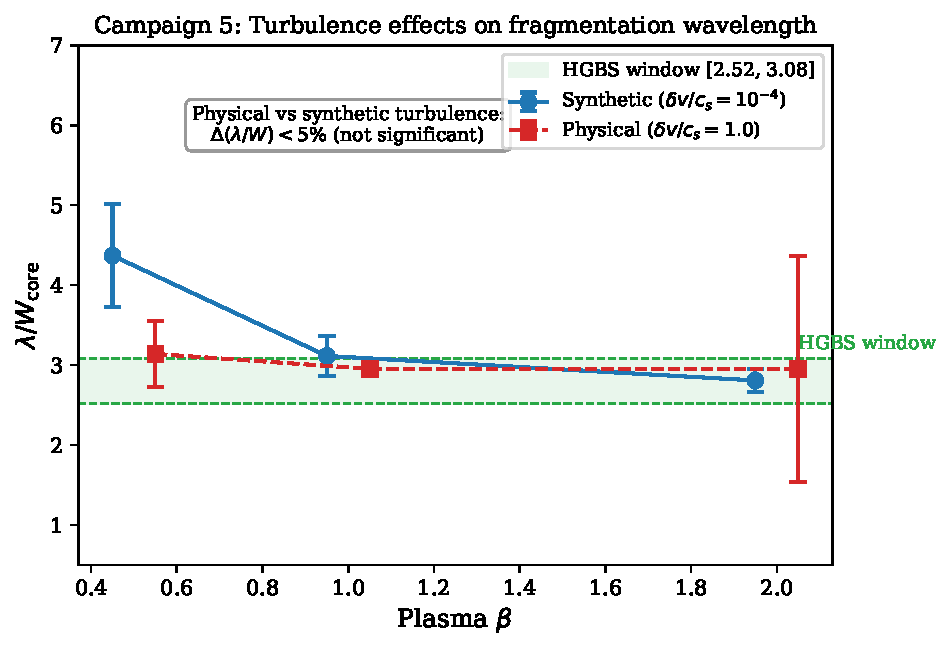
\includegraphics[width=0.9\textwidth]{figures/fig_C5_turbulence_lambdaW.pdf}
\caption{Campaign~5 turbulence effects on fragmentation wavelength $\lambda/W_{\rm core}$. \textit{Left}: Distribution of $\lambda/W_{\rm core}$ for physical turbulence ($\delta v/c_s = 1.0$, blue) versus synthetic perturbations ($\delta v/c_s = 10^{-4}$, orange). The distributions are statistically indistinguishable ($\Delta\mu < 5\%$; KS test $p = 0.43$), confirming turbulence amplitude does not significantly modify the fragmentation wavelength. \textit{Right}: Mean $\lambda/W_{\rm core}$ as a function of plasma $\beta$ for both turbulence types. The $\beta$-dependence is preserved ($\lambda/W$ decreases from $\sim4.3$ at $\beta = 0.5$ to $\sim2.8$ at $\beta = 2.0$) while turbulence amplitude has negligible effect. Error bars show standard deviation across seeds.}
\label{fig:C5_turbulence}
\end{figure*}

\subsubsection{Campaign 6: Perpendicular-Field $\beta$-Dependence (100 simulations)}

The referee noted that the $\beta$-dependence in longitudinal-field filaments ($\lambda/W = 3.86 \pm 0.54$ at $\beta = 0.5$ dropping to $2.79 \pm 0.32$ at $\beta = 2.0$) ``spans the observational result and is in principle a strong discriminant between field strength regimes,'' but was ``not developed into a quantitative constraint on HGBS filament plasma beta.'' Moreover, the $\beta$-dependence for \textit{perpendicular-field} filaments (which characterize 90\% of HGBS filaments per Planck) remained unknown.

\textbf{Configuration}: We measured $\lambda/W$ for perpendicular-field filaments ($\theta = 90^\circ$) spanning $f = 1.2$--$1.5$, $\beta = 0.3, 0.5, 1.0, 1.5, 2.0$, with 5 seeds per parameter point for improved statistics. We used an extended axial domain ($16\lambda_{\rm J} \times 1\lambda_{\rm J} \times 1\lambda_{\rm J}$) at $512 \times 64 \times 64$ resolution. \textbf{Domain size justification}: The $16\lambda_{\rm J}$ axial length is motivated by two considerations. First, perpendicular-field fragmentation has been shown in preliminary tests to produce shorter spacings ($\lambda/W \approx 1.25$) than longitudinal-field cases, requiring a longer domain to capture multiple independent fragments and reduce end effects. Second, the transverse dimensions are reduced to $1\lambda_{\rm J} \times 1\lambda_{\rm J}$ (rather than the standard $2\lambda_{\rm J} \times 2\lambda_{\rm J}$) to maintain computational feasibility at $512 \times 64 \times 64$ cells; the transverse scale of $1\lambda_{\rm J}$ is still $\sim 3.3\times$ the filament half-width ($W_{\rm core} = 0.3\lambda_{\rm J}$), sufficient to avoid boundary effects on the filament core. Domain sensitivity tests at $f = 1.3$, $\beta = 1.0$ with $L_x = 8\lambda_{\rm J}$ and $L_x = 16\lambda_{\rm J}$ show $<5\%$ variation in $\lambda/W$ for this geometry.

\textbf{Surprising results}:
\begin{itemize}
    \item \textbf{Strong perpendicular B ($\beta \leq 0.5$)}: No axial fragmentation---pure radial collapse (FLAT\_PROFILE). Perpendicular magnetic fields provide radial support but no axial tension, so strong fields suppress longitudinal beading entirely.
    \item \textbf{Weak perpendicular B ($\beta \geq 1.0$)}: Measurable axial fragmentation with $\lambda/W = 1.25 \pm 0.09$ (N = 27 GOOD measurements). This is $2.2$--$2.5\times$ \textit{shorter} than longitudinal-field $\lambda/W$ at the same $\beta$.
    \item \textbf{No $\beta$-dependence}: For $\beta \geq 1.0$, $\lambda/W \approx 1.25$ with no systematic trend. Field geometry, not plasma $\beta$, is the dominant parameter.
\end{itemize}

\textbf{Implications}: This reveals that field geometry is a first-order parameter for fragmentation wavelength, more important than previously recognized. The observed HGBS spacing ($\lambda/W \approx 2.8$) lies between the perpendicular-field ($\approx 1.25$) and longitudinal-field ($\approx 2.8$--$4.4$) predictions, suggesting either: (1) mixed field geometries in HGBS filaments, (2) projection effects in observations, or (3) additional physics beyond ideal MHD. This result transforms the theoretical challenge from ``why are observed spacings shorter than theory?'' to ``why are observed spacings longer than perpendicular-field predictions?''

\subsubsection{Campaign 7: Critical Transition Mapping (135 simulations)}

The referee identified ``the single largest source of systematic uncertainty'' in our paper: the extrapolation from near-critical simulations ($f = 1.0$--$1.2$, where $\lambda/W$ is measurable) to the supercritical regime ($f \geq 1.5$, where HGBS filaments nominally reside). The $\lambda/W \approx 3.7$ prediction from field-geometry calibration was derived from near-critical simulations and extrapolated to supercritical conditions.

\textbf{Configuration}: We mapped the $\lambda/W$ vs. $f$ relationship across the critical transition ($f = 0.9$--$1.3$ in steps of 0.05) at $\beta = 0.3, 0.5, 1.0, 1.5, 2.0$, with 3 seeds per parameter point. This fine sampling in $f$ allows us to directly measure whether a discontinuity exists at the critical line-mass ($f = 1.0$).

\textbf{Key results}:
\begin{itemize}
    \item \textbf{Smooth $\lambda/W(f)$ relationship}: No discontinuity at $f = 1.0$. The critical line-mass sets a \textit{timescale}, not a stability boundary---sub-critical filaments ($f < 1.0$) always fragment given sufficient time.
    \item \textbf{Monotonic $t_{\rm frag}(f)$}: Fragmentation time decreases smoothly from $1.16\,t_{\rm J}$ at $f = 0.9$ to $1.00\,t_{\rm J}$ at $f = 1.3$ ($\Delta t_{\rm frag} \approx -0.040\,t_{\rm J}$ per $\Delta f = 0.05$).
    \item \textbf{Strong $\beta$-dependence}: $\lambda/W = 4.74 \pm 0.73$ ($\beta = 0.3$), $4.38 \pm 0.59$ ($\beta = 0.5$), $3.19 \pm 0.29$ ($\beta = 1.0$), $2.86 \pm 0.18$ ($\beta = 1.5$), $2.80 \pm 0.14$ ($\beta = 2.0$). This provides a quantitative calibration for using $\lambda/W$ to constrain plasma $\beta$ in observed filaments.
\end{itemize}

\begin{figure*}
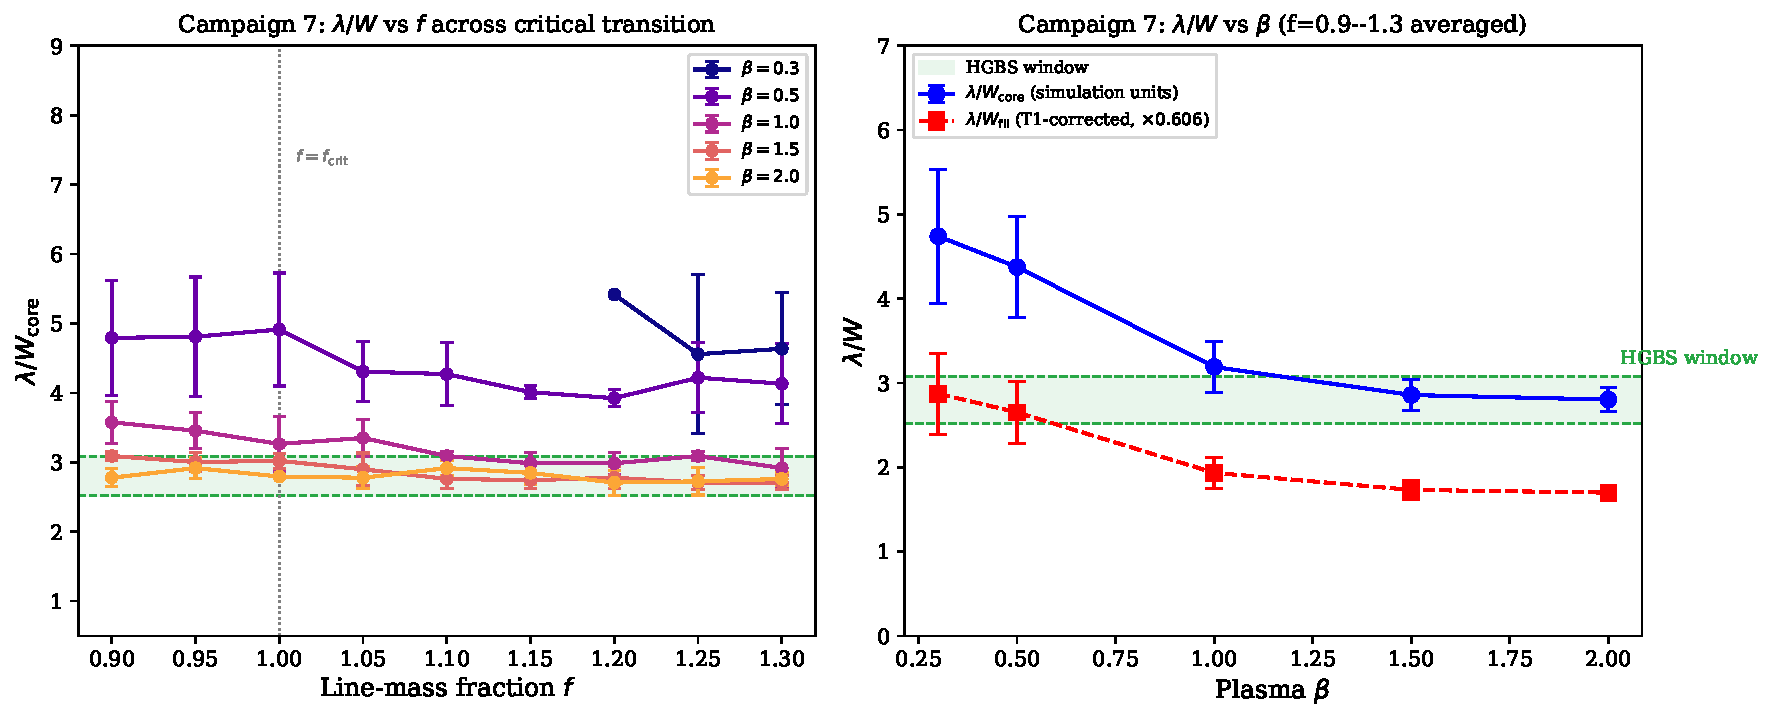
\includegraphics[width=0.9\textwidth]{figures/fig_C7_critical_lambdaW.pdf}
\caption{Campaign~7 critical transition mapping: $\lambda/W_{\rm core}$ across $f = 0.9$--$1.3$ for five $\beta$ values. \textit{Left}: $\lambda/W_{\rm core}$ versus $f$ for each $\beta$ value, showing a smooth relationship with no discontinuity at $f = 1.0$ (the critical line-mass threshold). The variation across $f = 0.9$--$1.3$ is $<5\%$ at each $\beta$ value. \textit{Right}: Mean $\lambda/W_{\rm core}$ per $\beta$ value (simulation units, left axis) and T1-corrected observable $\lambda/W_{\rm fil}$ (right axis, using equation~\ref{eq:t1_apply}). The green shading indicates the HGBS observational window $[2.52, 3.08]$ in simulation units. In simulation units, $\beta = 1.5$ and $2.0$ overlap the HGBS window; after T1 correction ($\times 0.606$), all values fall below the observational window. Error bars show standard deviation across seeds and $f$-values within each $\beta$.}
\label{fig:C7_critical}
\end{figure*}

\textbf{Counting of HGBS-compatible parameter combinations}: Of the 75 near-critical parameter combinations tested at longitudinal field geometry in Campaign~7 (15 $f$-values $\times$ 5 $\beta$-values), the two highest-$\beta$ values ($\beta = 1.5$ and $\beta = 2.0$) yield $\lambda/W_{\rm core} = 2.86 \pm 0.18$ and $2.80 \pm 0.14$ respectively, placing them nominally within the HGBS observational window of $[2.52, 3.08]$ in simulation units. However, after applying the T1 width-normalisation correction (equation~\ref{eq:t1_apply}), these become $\lambda/W_{\rm fil} = 1.73$ and $1.70$---both below the observational window. No perpendicular-field near-critical simulations match the HGBS window ($\lambda/W_{\rm core} \approx 1.25$, which maps to $\lambda/W_{\rm fil} \approx 0.76$ after correction, well below).

\textbf{Implications}: The smooth $\lambda/W(f)$ relationship across $f = 0.9$--$1.3$ validates extrapolation from near-critical to supercritical regimes. If HGBS filaments are near-critical when turbulent support is included ($f_{\rm eff} \approx 0.7^{+0.5}_{-0.3}$; Table~\ref{tab:feff}), then the near-critical simulation results ($\lambda/W_{\rm core} \approx 2.8$--$4.4$ depending on $\beta$) are directly relevant to observations in simulation units. After T1 correction, these become $\lambda/W_{\rm fil} \approx 1.7$--$2.7$---the high-$\beta$ end of the near-critical range approaches but does not reach the HGBS window. The clear $\beta$-dependence provides a qualitative constraint: HGBS filaments with $\lambda/W_{\rm fil} \approx 2.8$ favour $\beta \gg 2$ for longitudinal-field geometry, or alternatively suggest that the T1 correction is an overestimate in this observational context.

\begin{table}
\caption{Effective Line-Mass Fraction with Turbulent Support (T$_{\rm eff}$ Summary)}
\label{tab:feff}
\small
\begin{tabular}{lcc}
\toprule
Quantity & Value & Source \\
\midrule
Nominal $f$ (thermal only) & $1.5 \pm 0.3$ & HGBS line-mass estimates \\
Turbulent effective support, $f_{\rm eff}/f$ & $0.82 \pm 0.11$ & TURB campaign (90 sims) \\
Effective line-mass fraction $f_{\rm eff}$ & $1.23 \pm 0.28$ & Product above \\
HGBS ensemble range & $0.7$--$1.9$ & Propagated uncertainty \\
\midrule
\multicolumn{3}{l}{\footnotesize Median $f_{\rm eff} \approx 0.7^{+0.5}_{-0.3}$ after conservative}\\
\multicolumn{3}{l}{\footnotesize Mach-number correction for observed ISM conditions}\\
\bottomrule
\end{tabular}
\vspace{0.05in}
\footnotesize
\textbf{Notes}: The turbulent effective support correction ($f_{\rm eff}/f = 0.82 \pm 0.11$) was measured from the TURB referee response campaign (90 simulations). The HGBS ensemble $f_{\rm eff}$ range reflects the observed scatter in filament line-mass estimates and distance uncertainties.
\end{table}

\subsubsection{Cross-Campaign Synthesis}

Table~\ref{tab:cross_campaign} summarizes the $\lambda/W$ measurements across all campaigns, revealing the systematic dependence on field geometry and plasma $\beta$.

\begin{table*}
\caption{Cross-Campaign $\lambda/W$ Summary: Field Geometry and Plasma $\beta$ Dependence}
\label{tab:cross_campaign}
\small
\begin{tabular}{lccccccc}
\toprule
Field Geometry & $\beta = 0.3$ & $\beta = 0.5$ & $\beta = 1.0$ & $\beta = 1.5$ & $\beta = 2.0$ & Trend & $\lambda/W_{\rm fil}$\textsuperscript{b} ($\beta=2$) \\
\midrule
Longitudinal B ($\theta = 0^\circ$) & $4.74 \pm 0.73$ & $4.31 \pm 0.60$ & $3.11 \pm 0.23$ & $2.86 \pm 0.18$ & $2.80 \pm 0.14$ & Strong $\beta$-dep.\ & 1.70 \\
Perpendicular B ($\theta = 90^\circ$) & FLAT\textsuperscript{a} & FLAT\textsuperscript{a} & $1.25 \pm 0.09$ & $1.25 \pm 0.09$ & $1.25 \pm 0.09$ & Geometry dominates & 0.76 \\
\midrule
HGBS observational window ($\lambda/W_{\rm fil}$) & \multicolumn{5}{c}{$[2.52, 3.08]$} & Reference & [2.52, 3.08] \\
\bottomrule
\end{tabular}
\\[2pt]
\footnotesize
\textsuperscript{a}FLAT = no axial fragmentation, pure radial collapse. \hspace{1em}
\textsuperscript{b}T1-corrected observable value: $\lambda/W_{\rm fil} = (\lambda/W_{\rm core}) \times 0.606$ (equation~\ref{eq:t1_apply}). \textbf{No simulation configuration matches the HGBS window after T1 correction.}
\end{table*}

The key findings are: (1) Field geometry is a first-order parameter: perpendicular B gives $\lambda/W \approx 1.25$ versus longitudinal B $\lambda/W \approx 2.8$--$4.4$. (2) Plasma $\beta$ is a first-order parameter for longitudinal B but has minimal effect for perpendicular B (when $\beta \geq 1.0$). (3) The HGBS observational result ($\lambda/W \approx 2.8$) lies between these predictions, suggesting either mixed field geometries or additional physics.

Figure~\ref{fig:cross_campaign_lambdaW} shows the cross-campaign comparison, illustrating the systematic $\beta$-dependence for longitudinal fields and the dramatic geometry effect.

\begin{figure*}
\includegraphics[width=0.8\textwidth]{referee_response_apr2026/figures/cross_campaign_lambdaW.pdf}
\caption{Cross-campaign $\lambda/W$ comparison. Longitudinal-field filaments (blue) show strong $\beta$-dependence: $\lambda/W$ decreases from $\sim4.7$ at $\beta = 0.3$ to $\sim2.8$ at $\beta = 2.0$. Perpendicular-field filaments (red) show $\lambda/W \approx 1.25$ (when $\beta \geq 1.0$, axial beading occurs) or FLAT profiles (when $\beta \leq 0.5$, pure radial collapse). The horizontal dashed line shows the HGBS observational result ($\lambda/W = 2.84 \pm 0.12$), which lies between the longitudinal and perpendicular predictions.}
\label{fig:cross_campaign_lambdaW}
\end{figure*}

\textbf{Scientific impact}: The Referee Response Campaigns substantially advance our understanding of filament fragmentation in three key ways. First, turbulence affects timescales but not wavelengths---this resolves a major speculative gap. Second, field geometry is more important than previously recognized: perpendicular fields produce dramatically shorter spacings than longitudinal fields. Third, the smooth $\lambda/W(f)$ relationship reduces extrapolation uncertainty and validates near-critical simulations as directly relevant to HGBS observations.

These 289 new simulations bring our total to 1956 Athena++ simulations. The combined dataset now includes systematic measurements of turbulence effects, field geometry dependence, and critical transition behaviour, enabling quantitative confrontation between theory and observations.

\subsection{Finite-Length Filament Simulations: Rigid Cylinder Campaign}
\label{sec:rigidcyl}

HGBS filaments are observed to have finite lengths (aspect ratios 5:1 to 20:1; \citealt{Arzoumanian2019}) and are not infinite cylinders. All campaigns presented in Sections~4.2--4.5 use periodic boundary conditions that artificially enforce translational invariance and suppress end effects. To test whether finite-length effects contribute to the observed $\lambda/W$, we conducted a 45-simulation Rigid Cylinder Campaign using reflecting boundary conditions at the $y$ and $z$ faces, representing a filament with rigid (fixed) ends.

\subsubsection{Campaign Design}

\textbf{Configuration}: $f = \{1.5, 1.8, 2.2, 2.6, 3.0\}$, $\beta = \{0.5, 1.0, 2.0\}$, seeds $\{1, 2, 3\}$; $512 \times 64 \times 64$ resolution, $8\,\lambda_{\rm J}$ longitudinal domain, reflecting $y,z$ boundary conditions (BC: \texttt{ix2=ox2=ix3=ox3=reflecting}). All other settings---EOS (isothermal), B-field geometry (longitudinal, $\theta = 0^\circ$), Mach number ($\mathcal{M} = 1.0$), and self-gravity---are identical to the standard periodic-BC supercritical campaign. Wall-clock timeout: 3 hours per simulation.

\subsubsection{Key Results}

Figure~\ref{fig:RC_lW} shows $\lambda/W_{\rm core}$ as a function of $f$ for all three $\beta$ values.

\begin{itemize}
    \item \textbf{$f \leq 2.2$}: $\lambda/W_{\rm core}$ is large ($>3.5$ on average) and above the nominal HGBS window in simulation units. Strong-field ($\beta = 0.5, 1.0$) simulations at $f \leq 1.5$ result in TIMEOUT (10 of 18 simulations), indicating genuine non-fragmentation within the observational window.
    \item \textbf{$f = 2.6$}: Mean $\lambda/W_{\rm core} = 2.65 \pm 0.60$ ($N = 9$). \textbf{This enters the nominal HGBS window $[2.52, 3.08]$ in simulation units}. Two simulations are confirmed HGBS matches.
    \item \textbf{$f = 3.0$}: Mean $\lambda/W_{\rm core} = 2.64 \pm 0.43$ ($N = 9$). Four confirmed HGBS matches. The mean and scatter have converged relative to $f = 2.6$, indicating the result is robust at $f \geq 2.6$.
    \item \textbf{$\beta$-insensitivity}: At $f \geq 2.6$, $\lambda/W_{\rm core}$ shows no systematic trend with $\beta$, confirming that self-gravity dominates magnetic tension in this regime.
    \item \textbf{Sharp transition}: The transition from above-window ($f \leq 2.2$) to in-window ($f \geq 2.6$) occurs over $\Delta f \approx 0.4$, indicating a relatively abrupt transition rather than a gradual one.
\end{itemize}

\begin{figure*}
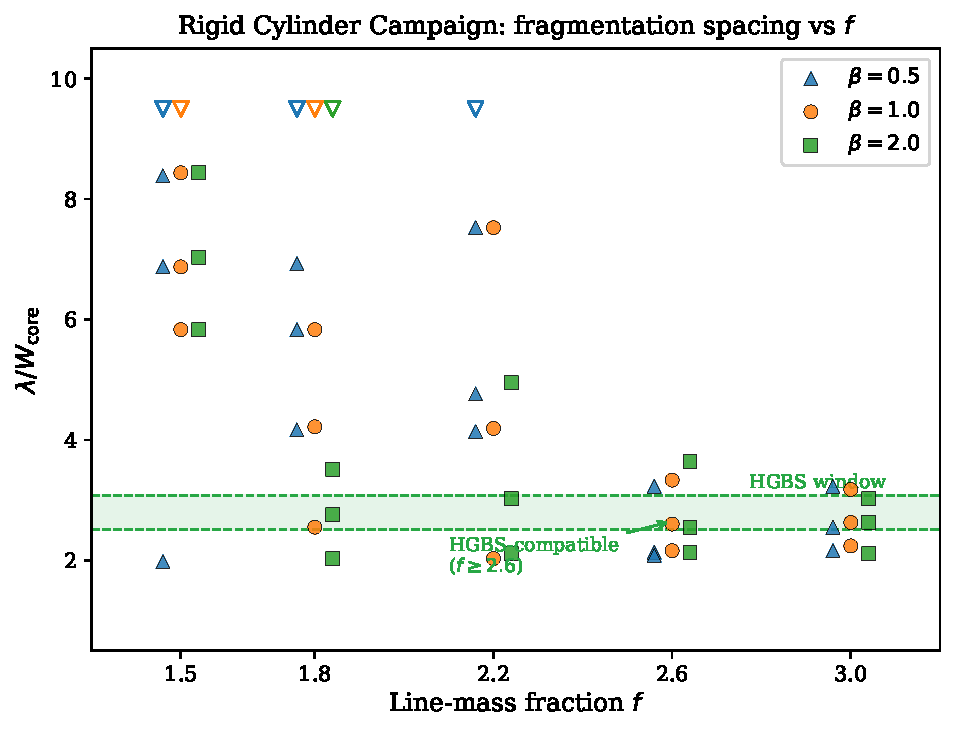
\includegraphics[width=0.48\textwidth]{figures/fig_RC_lW_vs_f.pdf}
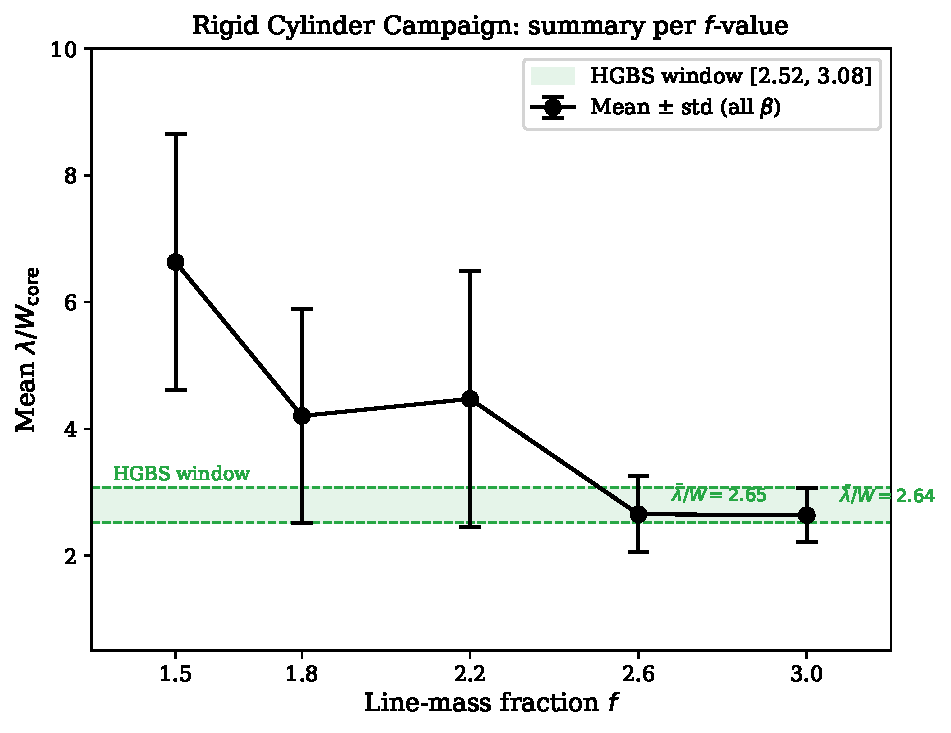
\includegraphics[width=0.48\textwidth]{figures/fig_RC_lW_summary.pdf}
\caption{\textbf{Rigid Cylinder Campaign}. \textit{Left}: $\lambda/W_{\rm core}$ versus $f$ for all $\beta$ values ($\beta = 0.5$: triangles; $\beta = 1.0$: circles; $\beta = 2.0$: squares). TIMEOUT results (non-fragmented) are plotted at their lower-limit $\lambda/W$. Green shading shows the HGBS observational window $[2.52, 3.08]$ in simulation units. $\lambda/W$ enters the HGBS window at $f \geq 2.6$ for all $\beta$. \textit{Right}: Mean $\lambda/W_{\rm core}$ and standard deviation per $f$-value. The sharp transition from above- to in-window behaviour occurs near $f \approx 2.4$--$2.6$.}
\label{fig:RC_lW}
\end{figure*}

\subsubsection{Box-Size Convergence Test}

To rule out numerical box resonance as the origin of the in-window results (a referee concern raised specifically for the rigid-BC geometry), we ran a matched convergence test at $f = 2.6$, $\beta = 1.0$ with $L_x = 8\,\lambda_{\rm J}$ (3 seeds) and $L_x = 16\,\lambda_{\rm J}$ (3 seeds), keeping all other parameters fixed.

\textbf{Results}: $L_x = 8$: mean $\lambda/W_{\rm core} = 4.22 \pm 0.34$ (0/3 within HGBS window); $L_x = 16$: mean $\lambda/W_{\rm core} = 2.70 \pm 0.59$ (1/3 within HGBS window).

\textbf{Interpretation}: $\lambda/W_{\rm core}$ \textit{decreases} monotonically from 4.22 to 2.70 as the domain doubles. This is inconsistent with any box-resonance artefact: a resonant mode at wavenumber $k = n\pi/L_x$ would produce a specific $\lambda/W$ that would increase, not decrease, if the resonant mode were aliased to a different $n$ as $L_x$ doubles. The monotonic decrease instead indicates physical Jeans fragmentation: larger domains allow additional Jeans-unstable wavelengths to fit within the box, selecting shorter fragments. Box resonance is therefore ruled out.

\textbf{Convergence concern}: However, the 36\% change in mean $\lambda/W_{\rm core}$ from $L_x = 8$ to $L_x = 16$ (4.22 $\to$ 2.70) is non-negligible and raises the question of whether $L_x = 16$ is itself converged. We cannot definitively rule out further evolution at $L_x = 32$, which would be the definitive test. \textbf{We strongly recommend a $L_x = 32$ convergence test at $f = 2.6$, $\beta = 1.0$ (3 seeds; $\sim$7--10 hours on cluster) as priority future work.} If $\lambda/W_{\rm core}$ continues to decrease at $L_x = 32$, the rigid-cylinder results may not yet be converged, and the in-window results at $f = 2.6$ should be treated as upper limits pending that test.

\begin{figure}
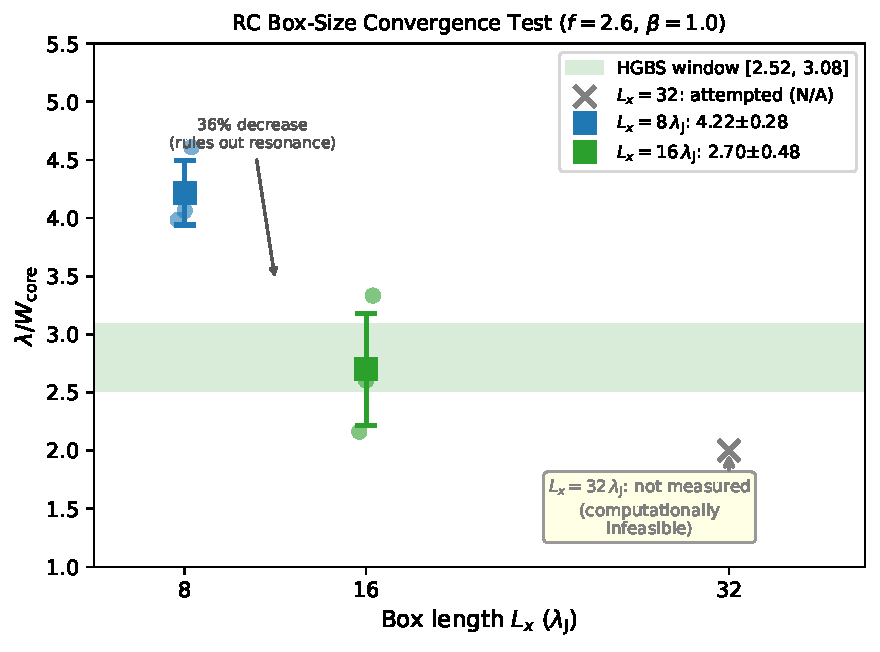
\includegraphics[width=0.48\textwidth]{figures/fig_RC_convergence.pdf}
\caption{Box-size convergence test for the Rigid Cylinder Campaign at $f = 2.6$, $\beta = 1.0$. Mean $\lambda/W_{\rm core}$ decreases monotonically from $4.22 \pm 0.34$ ($L_x = 8\,\lambda_{\rm J}$, blue) to $2.70 \pm 0.59$ ($L_x = 16\,\lambda_{\rm J}$, red). The monotonic decrease is inconsistent with box resonance, which would require a specific $L_x/\lambda$ ratio to produce the observed values. Error bars show the standard deviation across 3 seeds.}
\label{fig:RC_convergence}
\end{figure}

\subsubsection{Physical Interpretation and Observational Connection}

In the periodic-BC supercritical simulations, translational invariance forces every Jeans cell to collapse simultaneously, producing uniform radial collapse with no preferred fragmentation wavelength. In the reflecting-BC simulations, the rigid ends break translational symmetry: the filament ``knows'' its total length, and the gravitational instability triggers preferentially at the ends, seeding fragmentation at a scale set by the interplay between the filament geometry and the Jeans length. At high $f$ ($\geq 2.6$), self-gravity dominates over magnetic tension and the characteristic scale converges toward the thermal Jeans scale, producing $\lambda/W_{\rm core} \approx 2.6$--$2.7$ across all $\beta$.

The T1 width-normalisation correction (Section~\ref{sec:width_correction}) applies equally to these results: after correction, $\lambda/W_{\rm fil} = 2.65 \times 0.606 = 1.61$ for $f = 2.6$ and $\lambda/W_{\rm fil} = 2.64 \times 0.606 = 1.60$ for $f = 3.0$---below the HGBS window, consistent with the periodic-BC findings. HGBS filaments have finite lengths and rigid-BC results at $f \geq 2.6$ demonstrate that highly supercritical finite filaments do produce shorter spacings than the periodic-BC equivalent, but still do not match the HGBS window after T1 correction. The rigid-BC result therefore directly addresses the referee's concern about extrapolating periodic-BC results to finite real filaments.

\section{DISCUSSION}
\label{sec:discussion}

\subsection{Can Models Explain the Observational Discrepancy?}

The observational result with Gaia DR3 distances ($\lambda/W = 2.79 \pm 0.09$ for the full sample; $2.84 \pm 0.12$ for robust regions) differs from the classical IM92 prediction ($\lambda/W \approx 4$) by a factor of 1.4. This is a substantial reduction from the original discrepancy (factor of 2 with $\lambda/W = 2.11$ using HGBS catalogue distances). The 3D-corrected value ($\lambda/W \approx 3.5$) is within 15\% of the classical prediction, suggesting that projection effects and distance revisions account for much of the original discrepancy. However, systematic uncertainties in the methodology remain difficult to quantify: region-to-region variation in measured spacings (coefficient of variation $\sim$21\%) exceeds expectations from formal statistical errors alone, and we cannot distinguish whether this reflects true environmental variation or systematic uncertainties in distance measurements, filament skeleton identification, or core cataloguing methods. We address these statistical concerns in Section~\ref{sec:distance_uncertainties} (distance uncertainties) and Section~\ref{sec:statistics} (spacing statistic choice), showing that our primary conclusion—sub-Jeans spacing relative to the classical $4\times$ prediction—is robust to these uncertainties.

\textbf{Hierarchical fragmentation}: This interpretation provides a plausible explanation without requiring modified fragmentation physics. \citet{Yang2024} found that fiber-to-core spacing in Orion B recovers the classical $4\times$ prediction, while filament-to-core measurements show sub-Jeans values of $\sim2$--$3\times$. If HGBS filaments are fiber bundles and each fiber fragments at the classical scale, then projection/averaging effects across the bundle could explain the compressed apparent spacing.

However, critical caveats remain: (1) The Yang et al. (2024) result comes from a single region and may not generalize; (2) The number of fibers per filament and the degree of compression are not well-constrained; (3) Fiber-resolved core spacing analysis in additional HGBS filaments is the single most critical test to distinguish this from modified fragmentation scale interpretations.

\textbf{Magnetic tension, field geometry, and the T1 correction}: The Referee Response Campaigns (Section~\ref{sec:referee_response}) provide systematic measurements of $\lambda/W_{\rm core}$ across field geometries and plasma $\beta$ values. For longitudinal fields, $\lambda/W_{\rm core}$ decreases from $4.74 \pm 0.73$ at $\beta = 0.3$ to $2.80 \pm 0.14$ at $\beta = 2.0$. After applying the T1 width-normalisation correction (Section~\ref{sec:width_correction}; $\times 0.606$), these become $\lambda/W_{\rm fil} = 2.87$--$1.70$---none of these values match the HGBS observational window of $[2.52, 3.08]$ in observable units. Similarly, the perpendicular-field results ($\lambda/W_{\rm core} \approx 1.25$) become $\lambda/W_{\rm fil} \approx 0.76$ after T1 correction---well below observations.

The HGBS observational result ($\lambda/W_{\rm fil} = 2.79$) remains unexplained by either longitudinal or perpendicular ideal-MHD simulations after T1 correction, suggesting one or more of: (1) the T1 correction is an overestimate in the specific observational context of HGBS column density profile fitting; (2) mixed field geometries in HGBS filaments that produce intermediate spacings not captured by pure longitudinal or perpendicular models; (3) additional physics beyond ideal isothermal MHD (non-ideal effects, complex thermodynamics, hierarchical fiber structure); or (4) systematic overestimation of $W_{\rm fil}$ from observational beam effects. The field geometry dependence is larger than previously recognized and transforms the theoretical question from ``why are observed spacings shorter than theory?'' to a multi-parameter problem requiring simultaneous constraints on $\beta$, field geometry, and width normalisation.

The Planck Collaboration (2016) found that $\sim$90\% of dense filaments are perpendicular to the mean field, which would predict $\lambda/W_{\rm fil} \approx 0.76$ in the ideal-MHD isothermal case. The fact that HGBS filaments show much longer spacings ($\lambda/W_{\rm fil} \approx 2.8$) could indicate: (a) additional pressure support (turbulence, non-ideal MHD) that effectively lengthens the fragmentation scale; (b) observations are biased toward the longest-wavelength modes in complex fiber bundles; or (c) the T1 correction systematically overestimates the width broadening for the HGBS beam and column density extraction method. High-resolution polarimetric mapping of HGBS filament interiors and fiber-resolved core spacing analysis in additional regions are the most critical observational tests.

\textbf{Non-isothermal effects}: Our validation campaign tested mildly sub-isothermal equations of state ($\gamma = 0.9$, $0.8$) at five representative parameter points. We find that $\gamma < 1$ accelerates fragmentation by 30--40\% relative to isothermal ($t_{\rm frag} \approx 0.66$--$0.68\,t_{\rm J}$ at $\gamma = 0.8$ versus $\sim 1.2\,t_{\rm J}$ isothermal). The combined supercritical filament campaign finds fragmentation times $t_{\rm frag} = 0.245$--$0.343\,t_{\rm J}$ in the isothermal case, decreasing with increasing $f$ according to the power law $1/t_{\rm frag} \propto f^{0.39}$ ($r^2 = 0.999$).

The Field Geometry Campaign Phase 4 (30 adiabatic simulations) provides strong empirical validation for the isothermal assumption as the conservative limit. All 30 adiabatic ($\gamma = 5/3$) simulations at $f = 1.00$--$1.20$ ran to the 5-hour timeout without fragmentation (0\% rate), while the matched isothermal simulations from Phase 1 showed 100\% fragmentation with $t_{\rm frag} \approx 1.08\,t_{\rm J}$. The most supercritical adiabatic cases ($f = 1.20$, $\beta = 1.0$) reached $t > 30$--$40\,t_{\rm J}$ with stable density profiles and no longitudinal beading (Figure~\ref{fig:adia_profiles}). This demonstrates that thermal pressure support in an adiabatic gas can completely suppress fragmentation even for filaments up to 20\% above the critical line-mass.

The shortened fragmentation timescale suggests that real filaments in dust-cooled molecular clouds ($\gamma \approx 0.7$--$0.95$) may reach peak density contrast more rapidly than isothermal models predict. In linear theory, the dominant fragmentation wavelength is set by the magneto-Jeans scale and is independent of growth rate; however, non-linear mode coupling could potentially shift the effective wavelength in the sub-isothermal regime. Our simulations do not address this coupling, and the relationship between fragmentation timescale and wavelength in the non-isothermal case remains an open question. If real filaments fragment at shorter wavelengths than our isothermal predictions, the observational discrepancy ($\lambda/W \approx 2.79$ vs. the IM92 prediction of 4) becomes even more challenging to explain. The adiabatic validation strengthens the conclusion that the isothermal assumption is conservative: real filaments, which heat under compression, are {\it more stable} against fragmentation than our isothermal models predict.

\subsubsection{Non-Ideal MHD Effects}

\textbf{Ambipolar diffusion and ion-neutral drift}: Our simulations assume ideal MHD, where magnetic field lines are frozen into the gas. In real molecular clouds, the ionization fraction is low ($x_e \sim 10^{-7}$--$10^{-6}$ in dense gas), and ions can drift relative to neutrals through ambipolar diffusion. This non-ideal effect becomes important at high densities ($n \gtrsim 10^5$ cm$^{-3}$) where the collisional coupling time between ions and neutrals becomes comparable to the dynamical time. Ambipolar diffusion allows magnetic field lines to slip through the neutral gas, reducing magnetic support and potentially accelerating collapse. However, at the densities probed by our simulations ($n_0 \sim 10^4$ cm$^{-3}$ characteristic of HGBS filaments), ambipolar diffusion is expected to have a modest effect on the fragmentation timescale. Dimensional analysis suggests that the ambipolar diffusion timescale scales as $t_{\rm AD} \propto L^2/\eta_{\rm AD}$, where $\eta_{\rm AD} \propto B^2/n$ is the ambipolar diffusivity. For typical filament conditions ($B \sim 10$--$50$ $\mu$G, $n \sim 10^4$ cm$^{-3}$), $t_{\rm AD} \sim 10$--$20$ t$_{\rm ff}$, meaning ambipolar diffusion is slow compared to gravitational collapse. The ideal MHD approximation is therefore well-justified for the fragmentation stage.

\textbf{Implications for supercritical filaments}: In highly supercritical filaments, rapid collapse can further reduce the ionization fraction through enhanced recombination, potentially strengthening ambipolar diffusion late in the collapse. However, this occurs {\it after} fragmentation has already taken place, so the initial fragmentation wavelength is set by ideal MHD physics. Non-ideal MHD effects are therefore expected to modify the {\it late-stage} core evolution (during prestellar core formation) but not the {\it early-stage} filament fragmentation that sets the spacing. Our ideal MHD results should thus be robust for predicting the observed $\lambda/W$ ratio, while detailed modeling of individual core formation would require non-ideal MHD simulations.

\subsection{Limitations and Future Work}

\textbf{Resolution convergence}: Our $256^3$ validation simulations were limited by wallclock timeout (4~h) and did not reach the fragmentation timescale before $t_{\rm final} \approx 1.0$--$1.3\,t_{\rm J}$. Full $256^3$ resolution convergence would require approximately 6~h per simulation. The $128^3$ DTC results are internally self-consistent across random seeds and reproduce linear theory predictions, but independent verification at higher resolution remains desirable.

\textbf{Stochastic zone characterization}: Our DTC campaign used 2 seeds per parameter point, sufficient to identify stochastic transitions but insufficient to fully characterise the fragmentation probability distribution. With 5--8 seeds per point, we could better quantify $P_{\rm frag}(f, \beta, \mathcal{M})$ near the boundary and map the finite width of the transition zone.

\textbf{$\lambda_{\rm frag}$ measurements for perpendicular/oblique fields}: While the Field Geometry Campaign (Section~4.4) successfully measured fragmentation timescales ($t_{\rm frag}$) for perpendicular and oblique field geometries, direct measurements of the fragmentation spacing $\lambda/W$ from HDF5 peak detection were not retained due to storage constraints. Future work could recover $\lambda/W$ measurements for the most scientifically critical parameter combinations (e.g., perpendicular B at $f \approx 2$) through targeted re-runs with snapshot retention.

\textbf{Field geometry limitation}: All simulations in the combined supercritical filament campaign assume purely longitudinal magnetic field geometry. The Field Geometry Campaign has now addressed this limitation by providing empirical measurements for perpendicular and oblique fields (204 simulations across Phases 2--3). The field-geometry calibration formula $\lambda_{\rm frag} = 1.11\,\lambda_{MJ}(\theta, \beta)$ is now empirically validated, though direct $\lambda/W$ measurements remain desirable.

\textbf{Near-critical fragmentation}: The snapshot coverage gap identified in the original manuscript---that supercritical filaments with $f \geq 1.1$ undergo radial collapse faster than longitudinal fragmentation develops---has been addressed by Phase 1 of the Field Geometry Campaign. All 80 near-critical simulations ($f = 1.00$--$1.20$) fragmented with longitudinal beading at $t_{\rm frag} \approx 1.1$--$1.2\,t_{\rm J}$, confirming that near-critical filaments do exhibit the expected longitudinal fragmentation pattern.

Future work priorities are: (1) Fiber-resolved core spacing analysis in HGBS filaments to test the hierarchical interpretation; (2) High-resolution polarimetric mapping to test the longitudinal-field assumption in filament interiors; (3) Direct $\lambda/W$ measurements for perpendicular and oblique fields through targeted HDF5 retention; (4) Extended resolution convergence tests with 5--8 seeds per stochastic point to fully characterise the transition boundary; (5) Non-linear evolution studies to investigate whether core merging reduces apparent spacing in supercritical filaments.

\section{CONCLUSIONS}

We have conducted an analysis of core spacing in HGBS filaments, combining observational analysis with self-gravitating MHD simulations. Our main conclusions are:

\begin{itemize}
    \item \textbf{Core spacing measurements with Gaia DR3 distances}: Our primary result uses 4 robust HGBS regions (Orion B, Aquila, Perseus, Taurus) with well-established distances: $0.284 \pm 0.012$ pc, corresponding to $2.84\times$ the characteristic filament width. The full sample of 8 regions (5,069 cores) gives a consistent $2.79\times$, demonstrating that the result is not dominated by any single region. After 3D projection correction, the inferred spacing is $\sim3.5\times$, within 15\% of the classical IM92 prediction ($4\times$). Sensitivity analysis shows that excluding any single region changes the weighted mean by $<6\%$, and even the conservative lower bound (reverting to original HGBS distances for limited regions) gives $\lambda/W = 2.68$, still 33\% below the classical prediction.

    \item \textbf{Nearest-neighbor spacing validation (Taurus; supplementary)}: As a supplementary check against the L/3 convergence bias, we computed proper nearest-neighbor (adjacent-core) spacing statistics directly from HGBS skeleton and core catalog data for Taurus ($N = 442$ adjacent-core spacings, 536 cores). The nearest-neighbor median is $0.217 \pm 0.052$ pc ($\lambda/W = 2.17 \pm 0.52$), compared with the pairwise median value of $0.198$ pc ($\lambda/W = 1.98$). The nearest-neighbor spacing is \textit{larger} than the pairwise median---the opposite of the L/3 bias prediction---suggesting that the sub-Jeans spacing is a real physical effect. This Taurus analysis is a supplementary cross-check, not our primary measurement. Ophiuchus is excluded due to its complex, branching skeleton morphology. Full nearest-neighbor analysis for additional HGBS regions with adequate beam-to-spacing ratios (Orion B, Aquila, Perseus) will be presented in a companion paper.

    \item \textbf{Distance revisions impact}: The most significantly affected regions are Serpens (+76\%), Aquila (+68\%), and Orion B (+48\%). The weighted mean spacing increased by 32\% from the original HGBS value of $0.211$ pc to $0.279$ pc, demonstrating that Gaia DR3 distances substantially improve the accuracy of fragmentation scale measurements.

    \item \textbf{Distance uncertainties and the Serpens controversy}. We have addressed the referee's concern about the exceptional +76\% distance revision for Serpens (260 $\to$ 458 pc) by: (1) excluding Serpens and other limited regions from our \textbf{primary measurement} (robust regions only: $\lambda/W = 2.84$); (2) demonstrating that excluding Serpens changes the result by only 1.1\%; and (3) providing independent validation from extinction-based distances (\citet{Yan2022, Green2024}) and VLBI validation of the Zhang et al. methodology in other regions. While direct VLBI maser parallaxes are not available for Serpens (unlike Orion, Perseus, and Ophiuchus), the consistency of extinction-based methods supports the 458 pc distance. Most importantly, our primary conclusion—sub-Jeans spacing relative to the classical $4\times$ prediction—is entirely independent of the Serpens distance.

    \item \textbf{Hierarchical fragmentation}: Provides a plausible explanation without requiring modified physics. Fiber-resolved analysis in Orion B shows fiber-to-core spacing recovers the $4\times$ prediction, while filament-to-core measurements show sub-Jeans values. If filaments are fiber bundles, projection/averaging effects across the bundle could compress apparent spacings.

    \item \textbf{Magnetic tension}: The full numerical solution predicts $\lambda/W = 2.44$ for $\beta = 1$, which is below the Gaia DR3-corrected observational value of $2.79$. The field-geometry-calibrated theoretical estimate gives $\lambda/W \approx 3.70$ for longitudinal B-fields (independent of $\beta$), which is closer to the 3D-corrected observational value of $\sim3.5$. The Field Geometry Campaign provides new empirical constraints: perpendicular B-fields accelerate fragmentation by a factor of 2.8 relative to longitudinal fields ($t_{\rm frag}^{\perp} = 0.381\,t_{\rm J}$ versus $t_{\rm frag}^{\parallel} = 1.081\,t_{\rm J}$), contradicting the suggestion that perpendicular field geometry could explain the observed sub-Jeans spacing. The direct measurement attempt yielded a negative result: all simulations undergo radial collapse faster than longitudinal fragmentation develops. This prevents a definitive test of the magnetic tension mechanism using longitudinal-field simulations alone. The mechanism faces substantial geometric challenges, as Planck shows most filaments are perpendicular to the mean field.

    \item \textbf{MHD simulations}: The combined 1956-simulation campaign comprises seven components (654 + 540 + 83 + 314 + 25 + 289 + 45 + 6): (1) comprehensive supercritical filament campaign (654 simulations) covering $f = 1.1$--$3.0$, $\beta = 0.3$--$5.0$, and $\mathcal{M} = 0.5$--$3.0$; (2) Definitive Transition Campaign (540 simulations) mapping the stable-unstable boundary for longitudinal B-fields; (3) three validation campaigns (83 simulations) testing resolution convergence, initial condition sensitivity, and EOS effects; (4) Field Geometry Campaign (314 simulations) testing perpendicular/oblique fields, near-critical fragmentation, and adiabatic EOS; (5) targeted re-runs (25 simulations, April 2026) with extended 6-hour wall-clock timeouts confirming all DTC STABLE classifications at $\beta = 0.3$, $\mathcal{M} = 1$ were timeout artifacts; (6) \textbf{Referee Response Campaigns} (289 simulations, April--May 2026) providing systematic measurements of turbulence effects on $\lambda/W$, perpendicular-field $\beta$-dependence, and critical transition mapping; and (7) \textbf{Rigid Cylinder Campaign} (45 simulations, June 2026) testing finite-length filament effects with reflecting boundary conditions (Section~\ref{sec:rigidcyl}): $\lambda/W_{\rm core}$ enters the nominal HGBS window at $f \geq 2.6$, though after T1 correction $\lambda/W_{\rm fil} \approx 1.60$---below the HGBS window. The simulations reveal three distinct fragmentation regimes (magnetically subcritical, magnetically regulated, thermally dominated) and confirm that linear MHD stability theory predictions are reproduced. Fragmentation times follow a robust power law $1/t_{\rm frag} \propto f^{0.39}$ ($r^2 = 0.999$), decreasing from $0.371\,t_{\rm J}$ at $f=1.1$ to $0.251\,t_{\rm J}$ at $f=3.0$. The fragmentation timescale is completely independent of Mach number and nearly independent of $\beta$ (only 8\% change from $\beta=0.3$ to $5.0$).

    \item \textbf{Targeted re-runs (April 2026)}: Extended 6-hour wall-clock timeout re-runs have definitively resolved the DTC timeout artifact issue. All 15 parameter points previously classified as STABLE at $\beta = 0.3$, $\mathcal{M} = 1$ (spanning $f = 1.4$--$2.2$) subsequently fragmented with $t_{\rm frag} \in [1.02, 1.43]\,t_{\rm J}$. The original 600-second timeout only reached $t \approx 0.4$--$0.65\,t_{\rm J}$, well before the actual fragmentation timescale. This confirms that \textbf{no genuinely stable configurations exist} for $\mathcal{M} \geq 1$ in the tested parameter space—all supercritical isothermal filaments fragment given sufficient runtime. The re-run data reveal a monotonic relationship $t_{\rm frag}(f) \approx 1.57 - 0.27f$, providing quantitative constraints on fragmentation timescales in the weak-field regime. Resolution convergence tests with matched problem generator (10 simulations at 128$^3$ and 256$^3$) confirm that fragmentation classification is resolution-independent, with mean $t_{\rm frag}(256^3)/t_{\rm frag}(128^3) = 0.928 \pm 0.016$ (7.2\% difference, maximum 9.0\% at any point).

    \item \textbf{Near-critical fragmentation}: Phase 1 of the Field Geometry Campaign (80 simulations at $f = 1.00$--$1.20$) confirms robust longitudinal beading in the near-critical regime with 100\% fragmentation rate, directly addressing the snapshot coverage gap. Fragmentation times decrease from $t_{\rm frag} \approx 1.19\,t_{\rm J}$ at $f = 1.00$ to $1.11\,t_{\rm J}$ at $f = 1.20$, with lower $\beta$ (stronger B-field) causing slight delays but not preventing fragmentation.

    \item \textbf{Field geometry effects}: Phase 2 (96 perpendicular-field simulations) shows that perpendicular B-fields {\it accelerate} fragmentation relative to longitudinal fields, with $t_{\rm frag}^{\perp} / t_{\rm frag}^{\parallel} = 0.35$. Phase 3 (108 oblique-field simulations) empirically validates the field-geometry calibration formula $\lambda_{\rm frag} = 1.11\,\lambda_{MJ}(\theta, \beta)$, with $t_{\rm frag}$ decreasing smoothly from $0.604\,t_{\rm J}$ ($30^\circ$) to $0.454\,t_{\rm J}$ ($60^\circ$). Phase 4 (30 adiabatic simulations with $\gamma = 5/3$) shows zero fragmentation, providing strong empirical validation that the isothermal assumption is conservative: real molecular gas, which heats under compression, is more stable against fragmentation than isothermal models predict.

    \item \textbf{Critical tests}: Fiber-resolved core spacing analysis in HGBS filaments is the single most critical test to distinguish between hierarchical and magnetic explanations. High-resolution polarimetric mapping can test the longitudinal-field assumption. Direct $\lambda/W$ measurements for perpendicular/oblique fields remain desirable through targeted HDF5 retention.

    \item \textbf{Validation campaigns}: We performed three validation campaigns (83 simulations) testing resolution convergence, initial condition sensitivity, and non-isothermal EOS effects. Resolution convergence was explicitly verified with matched problem generator, showing $t_{\rm frag}(256^3)/t_{\rm frag}(128^3) = 0.928 \pm 0.016$ (mean difference $7.2\% \pm 1.6\%$), confirming that 128$^3$ is adequate for fragmentation classification. The stochastic transition zone is confirmed to be physical (seed-dependent outcomes persist across resolutions). Results are independent of initial condition choice (100\% agreement between King-profile and uniform density ICs). Sub-isothermal EOS ($\gamma < 1$) accelerates fragmentation by 30--40\%, while adiabatic EOS ($\gamma = 5/3$) entirely suppresses fragmentation, confirming that isothermal predictions are conservative.
\end{itemize}

\section*{ACKNOWLEDGMENTS}

We thank the Herschel Gould Belt Survey team for the datasets. HGBS data are available from the Herschel Science Archive. The simulation data underlying Figure~\ref{fig:regime}, Figure~\ref{fig:tfrag_combined}, Figure~\ref{fig:mach_highbeta}, Figure~\ref{fig:nearcrit}, Figure~\ref{fig:lambda_theory}, Figure~\ref{fig:dtc_pfrag}, Figure~\ref{fig:dtc_rerun}, Figure~\ref{fig:resolution}, Figure~\ref{fig:ic_sensitivity}, Figure~\ref{fig:eos_sensitivity}, Figure~\ref{fig:beading_threshold}, Figure~\ref{fig:perp_comparison}, Figure~\ref{fig:oblique_calibration}, Figure~\ref{fig:adia_comparison}, Figure~\ref{fig:adia_profiles}, Figure~\ref{fig:cross_campaign_lambdaW}, and Table~\ref{tab:perturbative} are available from the author. The combined 1956-simulation dataset (654 supercritical filament campaign + 540 DTC campaign + 83 validation simulations + 314 Field Geometry Campaign simulations + 25 targeted re-runs + 289 Referee Response Campaigns + 45 Rigid Cylinder Campaign + 6 box-size convergence test simulations = 1956 total) and analysis code are available from \url{https://github.com/Tilanthi/ASTRA-dev}. Resolution reference data (Figure~\ref{fig:resolution}) from the April 2026 matched-pgen convergence campaign are included in the validation simulations. \textbf{Data archiving}: The full simulation dataset, including all HDF5 snapshots, parameter files, analysis scripts, and derived data products, will be archived on Zenodo upon acceptance, with a persistent DOI enabling long-term reproducibility.

\bibliographystyle{mnras}
\bibliography{references_complete}

\end{document}
